\chapter{Constructing Synchronizing Transformations
   \pgsize{20 p.}
}
\label{chap:synchronization}

\todo{Vermeidbarkeit hängt insb. auch von der verwendeten Sprache ab. Z.B. sind Mappings / QVT-R analysierbar, aber Reactions / QVT-O nicht.}

\todo{Ergebnis sollte sein: Synchronisierungseigenschaft ist erreichbar per Konstruktuion}

\mnote{Transformation correctness can be achieved by adhering to the definition}
Transformations are the central artifacts of which a transformation network is composed.
We have introduced them as \emph{synchronizing transformations} in \autoref{def:synchronizingtransformation}, which are combinations of a consistency relation together with a consistency preservation rules that preserves it.
Correctness of such a transformation could then be defined as the property of the consistency preservation rule to preserve consistency of given models according to the consistency relation (cf.\ \autoref{def:synchronizingtransformationcorrectness}).
In theory, a correct transformation can simply be achieved by adhering to that definition.

%Even if we consider that one may only define a consistency preservation rule, which then induces the consistency relation as its image, thus being correct by construction, the rule may not behave as expected.

% Problem statement: Problem is a practical one, not a theoretical one.
% Ordinary transformations may be correct if used on their own (according to Stevens), but in context of a transformation network, when other transformation have modified the "target" model as well, they do not lead to a consistent result anymore, i.e., they are not correct.
% Start with example of duplicated creation and overwrite.

\mnote{Transformation languages base on unidirectional consistency preservation rules}
Using existing transformation languages, the defined transformations will, however, not follow the definition of a synchronizing transformation.
Transformation languages usually allow the specification of unidirectional consistency preservation rules, i.e., rules that restore consistency by updating one model if the other was modified.
Even if transformation languages allow bidirectional specifications, they still derive unidirectional consistency preservation rules from such a specification, such as forward and backward transformation (which may be incremental or not) derived from \glspl{TGG} rules~\cite{leblebici2014IncrementalTGGSurvey-GTVMT}.
In the following, we refer to such transformations as \emph{ordinary transformations} and give a more precise definition of them later on.
Synchronizing transformation, as we assume in transformation networks, are able to process changes made in both models and, in turn, also produce changes for both models.
This is an inevitable property in transformation networks, because both models involved in a transformation may have been modified due to different sequences of transformations having modified both of them.

\mnote{We want to find requirements to ordinary transformations to be used as synchronizing ones}
In this chapter, we aim to close this gap between synchronizing transformations as required in transformation networks and ordinary transformations with unidirectional consistency preservation rules used by transformation languages.
We investigate which requirements such an ordinary transformation has to fulfill to emulate a synchronizing transformation and thus be used in a transformation network.
This chapter thus constitutes our contribution \contributionref{contrib:correctness:synchronization}, which consists of three subordinate contributions: a discussion of the formal basis for the gap between synchronizing and ordinary transformations, a case distinction for synchronization scenarios in ordinary transformations, and finally techniques to build synchronizing transformations by ordinary ones.
\todo{Finally update goals}
It answers the following research question:

\researchquestionrepeat{rq:correctness:synchronization}

\mnote{Making ordinary transformations synchronizing enables reuse of languages and knowledge}
The benefit of enabling the definition of ordinary transformations that can be used a synchronizing ones instead of providing an approach or language for the specification of synchronizing transformations is that existing and well-researched transformation languages and knowledge about them can be reused.
Additionally, it reduces the complexity, because the definition of two unidirectional consistency preservation rules is less cumbersome than the definition of a single synchronizing transformation, which has to consider all possible combinations of changes in two models.
We will see that this is founded by the insight that only few combinations of changes are problematic and have to be explicitly considered.


%%%
%%% FORMAL GAP IDENTIFICATION
%%%
\section{Deriving the Gap to Ordinary Transformation}

%\todo{Exchange "ordinary" with "unidirectional"}
We have already introduced that there is both a formal and practical gap between synchronizing transformations, as we have defined as a component of transformation networks, and ordinary transformations, which are unidirectional and non-synchronizing, as used by most transformation languages.
In the following, we first give an example for faulty behavior if we simply used ordinary transformations in a transformation network.
Afterwards, we give a formal definition of unidirectional preservation rules and ordinary transformations, then defined as \emph{bidirectional transformations}.
Finally, we discuss the relation between unidirectional consistency preservation rules and unidirectional consistency relations as introduced in \autoref{chap:compatibility:formal_notion}.
%discuss options to sequence ordinary transformations and finally come up with a precise description of the formal gap and a practical approach to close it.


%%
%% MOTIVATING FAULT EXAMPLE WITH ORDINARY TRANSFORMATIONS
%%
\subsection{Behavior of Ordinary Transformations in Networks}
We have already sketched the example of creating a class in UML and Java after adding a component to a \gls{PCM} model in \autoref{chap:introduction:challenges:correctness:synchronization}.
In that scenario, it was possible that for a created \gls{PCM} component first a UML class is generated, which is then transformed into a Java class.
Additionally, the transformation between \gls{PCM} and Java creates another Java class, as it does not consider that there may be another transformation that already created that class.
Such scenarios can lead to the duplication of elements as an already existing element is inserted again, or to an overwrite of an already existing element.
Overwriting a previously created element may also overwrite and thus remove information that was already added to that it, like the transformation across UML may have added information to the Java class which is overwritten by new class creation of the transformation from PCM to Java.

\begin{figure}
    \centering
    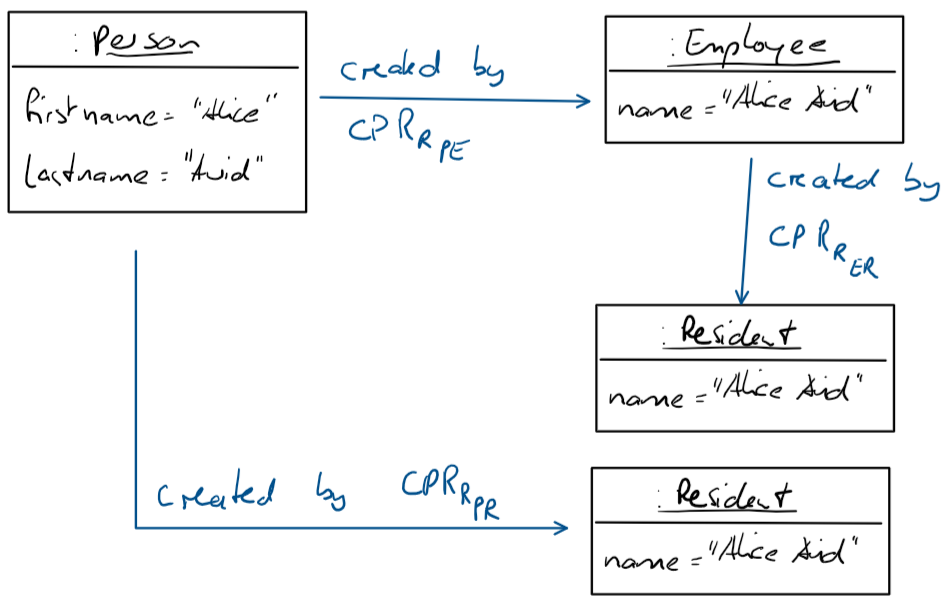
\includegraphics[width=0.8\textwidth]{figures/correctness/synchronization/duplicate_creation_example.png}    
    \caption{Duplicate creation of a resident by two sequences of consistency preservation rules}
    \label{fig:synchronization:duplicate_creation_example}
\end{figure}

An analogous example can be given for the running example of persons, employees and residents depicted in \autoref{fig:networks:three_persons_example}.
We consider the consistency relations $\consistencyrelation{R}{PE}, \consistencyrelation{R}{ER}$ and $\consistencyrelation{R}{PR}$.
As discussed in \autoref{chap:compatibility}, these relations are compatible, thus for any given person, employee or resident, there is a consistent set of models containing it.
Thus, the relations do not prevent transformations from finding consistent models whenever a person, employee or resident is added.
If we now consider ordinary transformations with unidirectional consistency preservation rules, they react to the changes in one model and update another accordingly.
In case of adding a person, this may look as depicted in \autoref{fig:synchronization:duplicate_creation_example}.
For each of the given consistency relations, we assume unidirectional consistency preservation rules that preserve consistency according to them.
They especially create an employee for each added person, and a resident for each created employee and person, respectively.
Since the transformations assume the models to be consistent before applying the changes, they always add a corresponding element when one of the elements is added.
This leads to the situation that both $\consistencypreservationrule{\consistencyrelation{CR}{ER}}$ as well as $\consistencypreservationrule{\consistencyrelation{CR}{PR}}$ create a resident upon creation of a person.
In consequence, there exist two residents with the same name, which does not fulfill the consistency relations.

It is our goal to find out how such a situation can be avoided by proper definition of consistency preservation rules in existing transformation languages.
A simple solution in this example would have been to look for the existence of elements to create first.
This can either be done by using a trace model, which most existing transformation language use to store corresponding elements, or by searching for an appropriate element in the other model.
Using a trace model, however, has some drawbacks and pitfalls, which we will investigate later.

% \begin{copiedFrom}{DocSym}

% % \section{Binary Transformation Interoperability}

% % Multi-model consistency preservation can be a achieved by combining binary transformations to graphs, %of transformations, 
% % with the transformations being executed transitively.
% % Since all binary transformations are developed independently of each other, it is necessary that they interoperate properly in a \emph{non-intrusive} way, thus without the necessity for the developer to understand and modify them, which we refer to as \emph{black-box combination}.

% Even under the assumption that, in contrast to our introductory motivation, all specifications are free of contradictions, it is easy to see that problems arise when combining binary transformations by transitively executing them.
% For example, consider the relations in \autoref{fig:prologue:binary_combination_example}.
% If a component is added to the \ac{ADL}, causing a \ac{UML} class creation due to \ref{fig:prologue:binary_combination_example:R1}, which in turn causes a Java class creation due to \ref{fig:prologue:binary_combination_example:R2}, the transformation for relation \ref{fig:prologue:binary_combination_example:R3} does not know that an appropriate class was already created, if the transformations are treated as black boxes.
% Consequently, the transformation will create the same class again, which may override the existing one, depending on the implementation and execution order.
% A simple solution for this example would be to have all transformations use a common trace model and check for existing elements before creating them in a transformation.
% Nevertheless, independently developed transformations will usually not assume that %this only applies if the transformation considers possibly preexisting transformation results, which it will not do in general if it does not assume other transformations to create corresponding elements.
% other transformations may already have created corresponding elements.
% Additionally, the trace model must allow the transformation engine to retrieve transitive traces.
% However, it is unclear if transitive resolution of traces can always be performed, as it can depend on whether the transitive trace belongs the considered consistency relation or another.
% %If, in another scenario, the transformation in the example was actually supposed to create an additional class, it would have to ignore the existing trace.

% As can be seen in the example, especially the correct handling of trace information in interdependent transformations has to be researched.
% This applies not only to element creations, but also other change types, such as attribute or reference changes, especially if they are multi-valued.
% In our thesis, we will therefore apply transitively executed binary transformations in different case studies to identify these and potential further problems.
% We then want to come up with a catalog of such problems %preventing the black-box combination of transformations 
% together with solution patterns for them.
% For example, to avoid duplicate element creations, a simple pattern could be to always check for already existing traces for that consistency relation in the transformations.
% In consequence, the integration of those patterns into a transformation language or the application of them as a transformation developer is supposed to achieve black-box combinability of the transformations.

% \end{copiedFrom} % DocSym


%%
%% USING FINE-GRAINED RELATIONS
%%
\subsection{Consistency Preservation for Fine-grained Relations}

\mnote{Consistency preservation defined for model-level consistency relations}
In our definition of consistency preservation rules in \autoref{def:consistencypreservationrule}, we used the coarse-grained notion of \modellevelconsistencyrelations, which describe consistency between two models in terms of a single relations.
In consequence, such a \modellevelconsistencypreservationrule ensures consistency to a single consistency relation.

\mnote{Fine-grained consistency relations allow to define relation between unidirectional preservation rules}
In \autoref{chap:compatibility:formal_notion}, we discussed that consistency relations can be considered in a fine-grained way that is able to reflect different notion of consistency in both directions between two models, such as a employee requiring a resident to exist but not vice versa.
We thus refined the notion of consistency relations in \autoref{def:consistencyrelation} to be defined unidirectionally and at the level of model elements rather than complete models.
%This fine-grained notion of consistency does also fit well to how specifications in transformation languages consider consistency, as they define rules that relate only some classes by relations or routines to preserve their consistency.
Since we also consider unidirectional consistency preservation rules as defined in transformation languages, we base further considerations regarding consistency preservation rules on such fine-grained and unidirectional consistency relations.
We later discuss how unidirectional consistency relations and unidirectional consistency preservation rules are related.
Nevertheless, we did also discuss in that chapter that each fine-grained relation can also be translated into a \modellevelconsistencyrelation, thus all insights we already had for those model-level relations still apply to the considerations regarding fine-grained ones.

\mnote{Transformation languages use fine-grained relations and preservation rules}
This fine-grained notion of consistency does also fit well to how specifications in transformation languages consider consistency.
They allow to define rules that relate only some classes by relations, conforming to fine-grained consistency relations, from which then fine-grained consistency preservation rules are derived, or they directly allow to define routines to preserve consistency between specific classes.
These rules are often called \emph{transformation rules} and composed to a transformation that consists of multiple such rules, each encoding a consistency relations and a preservation rule for it.
%We will, however, stick to the coarse-grained notion of consistency preservation rules, because, first, it is difficult to describe how such fine-grained consistency preservation rules can be composed, and second, the coarse-grained notion is sufficient for our considerations anyway.

\mnote{Stick to coarse-grained notion of preservation rules}
It may easily happen that the execution of one transformation rule leads to the violation of the consistency relation of another one, which introduced dependencies between the individual transformation rules.
Thus, a combination of such transformation rules to a transformation has to ensure correctness, i.e., that the consecutive execution of the rules leads to a consistent state of the models.
Languages such as \gls{QVTR} and \gls{QVTO} therefore specify that transformation rules may not be conflicting (cf. \cite[7.10.2.]{qvt}).
It is also a dedicated topic of research to ensure that the rules of a single transformation conform to each other, e.g.\ \cite{cuadrado2017tse,cabot2010jss}, thus we assume that a transformation has that property.
To avoid the necessity of specifying this conformance property for transformation rules, we stick to the existing notion of coarse-grained consistency preservation rules, as it is sufficient for our considerations.

\mnote{New transformation notion based on fine-grained consistency relations}
In consequence, from now we consider a synchronizing transformation as a set of fine-grained consistency relations according to \autoref{def:consistencyrelation} and a consistency preservation rule that preserves consistency according to the set of relations $\consistencyrelationset{CR}$ rather than a single \modellevelconsistencyrelation $\consistencyrelation{CR}{}$.
A consistency preservation rule $\consistencypreservationrule{\consistencyrelationset{CR}}$ and also a transformation with that preservation rule are thus still considered correct if it is applied to a consistent pair of models and changes to them and applying the resulting changes to the models again delivers a pair of models that is consistent to all consistency relations, i.e.:
\begin{align*}
    &
    \forall \model{m}{1} \in \metamodelinstanceset{M}{1}, \model{m}{2} \in \metamodelinstanceset{M}{2}, \change{\metamodel{M}{1}} \in \changeuniverse{\metamodel{M}{1}}, \change{\metamodel{M}{2}} \in \changeuniverse{\metamodel{M}{2}} : \tupled{\model{m}{1},\model{m}{2}} \consistenttomath \consistencyrelationset{CR} \\
    & \formulaskip
    \land \exists \change{\metamodel{M}{1}}' \in \changeuniverse{\metamodel{M}{1}}, \change{\metamodel{M}{2}}' \in \changeuniverse{\metamodel{M}{2}} : \tupled{\change{\metamodel{M}{1}}', \change{\metamodel{M}{2}}'} = \consistencypreservationrule{\consistencyrelationset{CR}}(\model{m}{1}, \model{m}{2}, \change{\metamodel{M}{1}}, \change{\metamodel{M}{2}}) \\
    & \formulaskip\formulaskip
    \Rightarrow \tupled{\change{\metamodel{M}{1}}'(\model{m}{1}),\change{\metamodel{M}{2}}'(\model{m}{2})} \consistenttomath \consistencyrelationset{CR}
\end{align*}
Note that being consistent to all fine-grained consistency relations is equivalent to being consistent to the single \modellevelconsistencyrelation induced by the fine-grained relations.

% In our definition of consistency preservation rules in \autoref{def:consistencypreservationrule}, we used the coarse-grained notion of \modellevelconsistencyrelations and, accordingly, defined \modellevelconsistencypreservationrules that consider models as whole.
% We refined the notion of consistency relations in \autoref{def:consistencyrelation} to be defined at the level of model elements rather than complete models.
% This fine-grained notion of consistency fits well to how specifications in transformation languages consider consistency, as they define rules that relate only some classes by relations or routines to preserve their consistency.
% In the following, we thus also stick to this fine-grained notion of consistency.
% We will, however, stick to the coarse-grained notion of consistency preservation rules given in \autoref{def:consistencypreservationrule}

% \subsection{Feingranulare CPR}
% Jede CPR stellt Konsistenz bzgl. einer unidirektionalen CR wieder her.
% Ein CPR darf keine Änderung machen, die eine andere CR verletzt.
% Schwierig, da CPR voneinander abhängen können (was wiederum dagegen spricht, dass eine CPR nicht eine andere CR verletzen darf), wie also Reihenfolge festlegen?
% Ist keine Option, insbesondere Annahme, dass sich CPR nicht gegenseitig beeinflussen nicht nachvollziehbar (obwohl in der Praxis dasselbe Probleme existiert, da CPR sowieso in feingranulare Regeln zerlegt werden, die natürlich widersprüchlich sein könnten).

%\todo{Relate to the circumstance that we want to consider unidirectional preservation rules, so unidirectional rules might be interesting. We will later find, that this is not the case}


%%
%% UNIDIRECTIONAL CONSISTENCY PRESERVATION RULES
%%
\subsection{Unidirectional Consistency Preservation Rules}

\mnote{Formal definition of unidirectional consistency preservation rules}
Before we can discuss options how unidirectional consistency preservation rules can be used to emulate the behavior of synchronizing consistency preservation rules, we first need to define them to be able to formally compare the two of them.
In contrast to a synchronizing consistency preservation rule as defined in \autoref{def:consistencypreservationrule}, a unidirectional consistency preservation rule does only receive changes made to one of the two models and returns changes to the other models instead of receiving and returning changes to both.

\begin{definition}[Unidirectional Consistency Preservation Rule]
    \label{def:unidirectionalconsistencypreservationrule}
    Let $\metamodel{M}{1}, \metamodel{M}{2}$ be two metamodels and $\consistencyrelationset{CR}$ a set of consistency relations between elements of those metamodels.
    A \emph{unidirectional consistency preservation rule} $\consistencypreservationrule{\consistencyrelationset{CR}}$ for the relation set $\consistencyrelationset{CR}$ is a (usually partial) function:
    \begin{align*}
        \consistencypreservationrule{\consistencyrelationset{CR}} : (\metamodelinstanceset{M}{1}, \metamodelinstanceset{M}{2}, \changeuniverse{\metamodel{M}{1}}) \rightarrow \changeuniverse{\metamodel{M}{2}} \cup \setted{\bot}
    \end{align*}
\end{definition}

\mnote{Preservation rules as defined in or derived from transformation languages}
This is how the consistency preservation rules defined in or derived from existing transformation languages operate.
They take two models and changes to one of them and generate changes for the other.
Most of them even directly apply the changes instead of returning a dedicated change artifact.
If the rule is not able to handle the given changes, it may return $\bot$.

\mnote{Correctness of unidirectional rules analogous to common notions}
In addition, they usually assume the input models to be consistent and then ensure that applying the input and the output changes to the models, the resulting models are consistent again.
This conforms to the common notion of \emph{correctness} for consistency preservation rules, like for the state-based (rather than our delta-based) notion of consistency preservation rules defined in \cite{stevens2010sosym}.
This is even compliant to the correctness notion that we defined for synchronizing consistency preservation rules in \autoref{def:consistencypreservationrulecorrectness}.
Thus, we define correctness of such a unidirectional consistency preservation rule as follows.

\begin{definition}[Unidirectional Consistency Preservation Rule Correctness]
    \label{def:unidirectionalconsistencypreservationrulecorrectness}
    Let $\consistencypreservationrule{\consistencyrelationset{CR}}$ be a unidirectional consistency preservation rule.
    We call $\consistencypreservationrule{\consistencyrelationset{CR}}$ \emph{correct} if the resulting models when applying the generated changes are consistent to $\consistencyrelationset{CR}$ again:
    \begin{align*}
        &
        \forall 
        \model{m}{1} \in \metamodelinstanceset{M}{1}, 
        \model{m}{2} \in \metamodelinstanceset{M}{2},
        \change{\metamodel{M}{1}} \in \changeuniverse{\metamodel{M}{1}} : \\
        & \formulaskip
        \bigl( \tupled{\model{m}{1}, \model{m}{2}} \consistenttomath \consistencyrelationset{CR} \\
        & \formulaskip
        \land \exists 
        \change{\metamodel{M}{2}} \in \changeuniverse{\metamodel{M}{2}} :
        \change{\metamodel{M}{2}} = \consistencypreservationrule{\consistencyrelation{CR}{}}(\model{m}{1}, \model{m}{2}, \change{\metamodel{M}{1}}) \bigr) \\
        & \formulaskip\formulaskip
        \Rightarrow
        \tupled{\change{\metamodel{M}{1}}(\model{m}{1}), \change{\metamodel{M}{2}}(\model{m}{2})} \consistenttomath \consistencyrelationset{CR}
    \end{align*}
\end{definition}

\mnote{Synchronizing consistency preservation rules can be partial}
In \autoref{def:unidirectionalconsistencypreservationrule}, we explicitly allow consistency preservation rules to be partial.
This was only an optional requirement for synchronizing consistency preservation rules defined in \autoref{def:consistencypreservationrule}, because there may be changes to both models which cannot be processed reasonably as one the changes may need to reverted to achieve consistency.
Ignoring that practical requirement, it is theoretically possible to always return changes that, if applied to the input models, produce consistent models.
Those returned changed may perform arbitrarily unreasonable modifications, but still restore consistency.

\mnote{Unidirectinoal consistency preservation rule must be partial}
In general, unidirectional consistency preservation rules need to be partial.
This is due to the reason that there can be models for which no other models can be generated such that they are consistent with respect to a set of consistency relations.
Consider the consistency relations $\consistencyrelation{CR}{} = \setted{\tupled{a, z}, \tupled{b, z}}$ and its transposed $\consistencyrelation{CR}{}^T = \setted{\tupled{z, a}, \tupled{z, b}}$.
If a change generated the model $\model{m}{} = \setted{a, b}$, then no consistent model can be generated.
A consistent model would have to contain $z$, because the consistency relation $\consistencyrelation{CR}{}$ requires for $a$ and $b$ an element $z$ to exist in the other model.
The consistency relation $\consistencyrelation{CR}{}^T$, however, requires that for a $z$ only either $a$ or $b$ exists in the other model, as otherwise no witness structure with unique corresponding elements can be found (see \autoref{def:consistency} for consistency).
In consequence, a unidirectional consistency preservation rule may not produce a result for such an input and thus be partial, as the result would never fulfill the correctness definition.

In fact, the definition does not specify for which inputs a unidirectional consistency preservation rule is allowed to be undefined.
One could restrict this behavior to cases in which there is no $\change{\metamodel{M}{2}} \in \changeuniverse{\metamodel{M}{2}}$ for given models $\model{m}{1}$ and $\model{m}{2}$ as well as change $\change{\metamodel{M}{1}} \in \changeuniverse{\metamodel{M}{1}}$, such that $\tupled{\change{\metamodel{M}{1}}(\model{m}{1}), \change{\metamodel{M}{2}}(\model{m}{2})} \consistenttomath \consistencyrelationset{CR}$ for a set of consistency relation $\consistencyrelationset{CR}$.
We, however, leave it up to the developer to decide for which inputs a consistency preservation rule is undefined, as there might be cases in which a change that restores consistency can be restored, but does semantically not make this.
This was also the reason for allowing a synchronizing consistency preservation rule to be partial, which is why we have already discussed the scenario in \autoref{chap:correctness:formalization:incremental_inductive}.
% \subsection{Partial Definition of Consistency Preservation Rules}
% \todo{Move this to definition of unidirectional preservation rules?}
% 1. Schon eine synchronisierende Transformation muss nicht für jede Eingabe definiert sein. Es könnte natürlich sein, dass sich gleichzeitige Änderungen nicht sinnvoll in Einklang bringen lassen. Theoretisch ist es aber möglich eine total definierte Funktion anzugeben, da immer ein beliebigen (im dümmsten Fall immer dasselbe / leere Modell) zurückgeliefert werden kann.


%%
%% NONALIGNMENT OF UNIDIRECTIONAL CONSISTENCY RELATIONS AND UNIDIRECTIONAL CONSISTENCY PRESERVATION RULES
%%
\subsection{Unidirectional Relations and Preservation Alignment}
\label{chap:synchronization:gap:alignment}

\mnote{Unidirectional consistency preservation rules for each unidirection consistency relation}
Defining unidirectional consistency preservation rules based on a unidirectional notion of consistency relations imposes the idea of having one unidirectional consistency preservation rule associated with one unidirectional consistency relation, or at least a set of unidirectional relations between the same two metamodels.
In consequence, we would have two sets of unidirectional consistency relations between two metamodels and a consistency preservation rule for each of them.

\begin{figure}
    \centering
    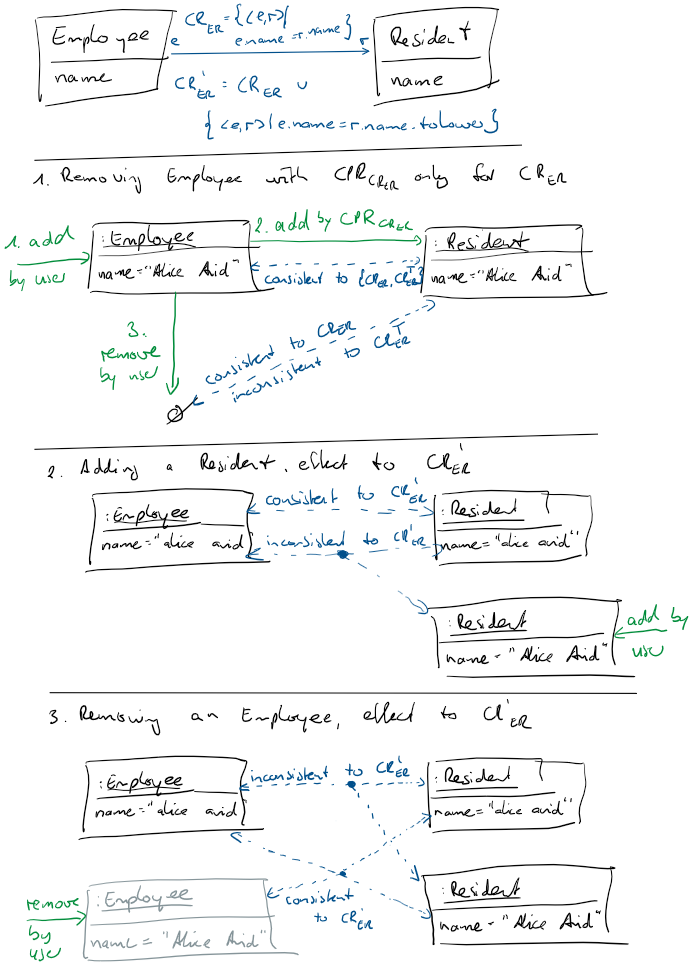
\includegraphics[width=0.9\textwidth]{figures/correctness/synchronization/unidirectional_nonalignment.png}
    \caption[Nonalignment of Unidirectional Relations and Preservation Rules]{Nonalignment of Unidirectional Relations and Preservation Rules. %: scenario for unidirectional consistency preservation rule requiring knowledge about consistency relation in opposite direction (1)
    }
    \todo{Split into two figures}
    \label{fig:synchronization:unidirectional_nonalignment}
\end{figure}

\mnote{Unidirectional consistency preservation rules cannot only consider one direction of consistency relations}
It is, however, easy to see that a unidirectional consistency preservation rule cannot only consider one direction of consistency relations, but needs to consider both.
Consider the example in \autoref{fig:synchronization:unidirectional_nonalignment}, which contains an extract of the consistency relations of the running example.
We assume the consistency relations $\consistencyrelation{CR}{ER}$ and $\consistencyrelation{CR}{ER}^T$ describing that for each employee a single corresponding resident must exist and vice versa.
As discussed before, only considering $\consistencyrelation{CR}{ER}$ would realize the notion of not requiring an employee for every resident.
If we define a unidirectional consistency preservation rule $\consistencypreservationrule{\consistencyrelation{CR}{ER}}$ only for the consistency relation $\consistencyrelation{CR}{ER}$ with the goal to always preserve consistency according to that relation after changes to the employee model, the example scenario 1 in \autoref{fig:synchronization:unidirectional_nonalignment} show that this is not the case.
While for the scenario of adding an employee the rule properly propagates the change by adding a resident and thus restores consistency, removing an employee leads to a violation of consistency.
Removing an employee does not require the consistency preservation rule to perform any changes in the resident model, because $\consistencyrelation{CR}{ER}$ only requires a unique resident to exist for every employee, but does not forbid that there is a resident for which no employee exists.
This is defined by the inverse relation $\consistencyrelation{CR}{ER}^T$.
In consequence, after removing tan employee the consistency preservation rule does not perform any changes, as consistency to $\consistencyrelation{CR}{ER}$ is given, but the model are then inconsistent to $\consistencyrelation{CR}{ER}^T$.

\mnote{Changes to one model may affect consistency relations in both directions}
The given scenario exemplifies the general case that a consistency according to a consistency relation cannot only be violated by performing changes to the model containing the left condition elements of the relations, but also by changes to the model containing the right condition elements of the relation.
In general, consistency of models according to a consistency relation is affected by the presence of condition elements in the models.
Consistency is defined as the ability to find a witness structure, i.e., a unique mapping between condition elements of the consistency relation that occur in the models.
Thus, adding, changing or removing elements in model that constitute a condition element of the consistency relations can lead to inconsistencies.

\mnote{Distinction of addition, removal or change of condition elements for consistency relation affection}
We can see that any type of change can lead to the violation of a consistency relation in either direction:
\begin{properdescription}
    \item[Addition:] Whenever a condition element of the left side of a consistency relation is added to a model, a corresponding condition element need to exist in the other model. If it does not exist yet, the models are not consistent to that relation.
    When a condition element of the right side of a consistency relation is added to a model, this does, according to the definition of consistency, not require another condition element to exist in the other model. It can, however, lead to the situation that no witness structure with a unique mapping between the elements exists anymore.
    Consider the exemplary relation $\consistencyrelation{CR}{ER}'$ in \autoref{fig:synchronization:unidirectional_nonalignment} and the example scenario 2.
    Having an employee with name \enquote{alice avid} and a corresponding resident with the same name, the models are consistent to that relation.
    Adding a resident with name \enquote{Alice Avid} violates $\consistencyrelation{CR}{ER}'$, because the employee \enquote{alice avid} corresponds to both residents, so there is no mapping inducing a witness structure for consistency.
    In consequence, adding a right side condition element of the consistency relation to the models can also violate consistency to a consistency relation.
    \item[Removal:] Whenever a condition element of the right side of a consistency relation is removed from a model, the corresponding condition element in the other model still exists. Because this element does not necessarily have a corresponding one anymore, there may not be a valid witness structure and thus the models may not be consistent anymore.
    When a condition element of the left side of a consistency relation is removed from a model, the originally corresponding element is not connected to the removed element in the witness structure anymore. If another element is considered to this corresponding element, there is no unique mapping of elements anymore.
    Consider again the relation $\consistencyrelation{CR}{ER}'$ in \autoref{fig:synchronization:unidirectional_nonalignment} and the example scenario 3.
    Having two employees and residents with the names \enquote{alice avid} and \enquote{Alice Avid}, the models are consistent because each employee has a corresponding resident and vice versa.
    If we remove the employee \enquote{Alice Avid}, the models are consistent to $\consistencyrelation{CR}{ER}'$ anymore, because the remaining employee corresponds to both residents, so there is no unique mapping of condition elements.
    \item[Change:] We do not have a precise notion of when a condition element can be considered changed, as elements do not have identity. 
    Additionally, consistency in terms of being able to find a witness structure is only based on the existence or non-existence of condition elements, thus whether an element was changed or removed and created makes no different.
    We might say that a condition element can be considered changed when the change describes modifications of the model elements in the condition element that lead to a new condition element within the same condition.
    This does, conceptually, not different from the removal of one and the addition of another condition element.
    Thus, the same situations as discussed for addition and removal above can occur.
\end{properdescription}

\mnote{Unidirectional consistency preservation rules cannot be synchronizing}
%In addition to the insight that unidirectional consistency preservation rule must base on all consistency relations between two metamodels rather than only the ones in a specific direction, 
It is also easy to see that there is no trivial way of specifying a unidirectional synchronizing consistency preservation rule.
It may seem natural to define a consistency preservation rule that is able to process changes in both models and then return only changes in one of them to restore consistency to close the gap between synchronizing and ordinary transformations.
Consider the situation that we have two residents and employees named \enquote{Alice Avid} and \enquote{Bob Do}.
If one of them is removed in the residents model and the other in the employees model, then a proper synchronizing transformation should remove both corresponding elements such that the models are empty.
This requires changes to both models.
With a synchronizing unidirectional consistency preservation rule for each direction, neither of them can produce changes in one of the models that reasonably restore consistency.
Such a rule would necessarily revert one removal to restore consistency, which is not the intended behavior and would probably not be specified by a developer that way, such that the consistency preservation rule would be undefined for that input, although a synchronization transformation would be able to resolve those changes.
In fact, we would expect to have two unidirectional consistency preservation rules of which each removes one of the elements.
This does, however, violate our existing notion of correctness for a single consistency preservation rule.
In the subsequent sections, we will therefore discuss relaxed requirements to unidirectional consistency preservation rules to be able to act like a synchronizing transformations.

% A unidirectional consistency relations require preservation rules in both directions (add/delete)
% \begin{itemize}
%     \item A single unidirectional consistency relation may impose preservation rules in both directions: For each employee, a resident is required, but not every resident needs to be an employee. When then have only one unidirectional consistency relation describing that circumstance. We need, however, consistency preservation rules in both directions, because if, for example, a resident is removed, the employee needs to be removed as well, whereas a resident has to be added whenever an employee is added.
%     \item With ordinary unidirectional rules, we then have that after a change to model 1, the unidirectional rule has to change model 2 so that they are consistent to both unidirectional relations (and vice versa)
% \end{itemize}
% Konsequenz: Wir können nicht für die unidirektionalen Konsistenzrelationen jeweils die CPR in die Richtung angeben, sondern jede unidirektionale CPR muss immer die Konsistenzrelationen in beide Richtungen berücksichtigen.

% Define mapping between change types and directionality of involved consistency relation (delete in opposite direction than add or modification). Make example at witness structures.

% Beachten, dass auch beim Hinzufügen in m2 die Relation m1->m2 verletzt werden kann, da nun zu viele Elemente vorhanden sind -> keine Witness-Struktur.


% \paragraph{Synchronizing Transformation cannot be Unidirectional}
% Es ist einfach zu sehen, dass synchronisierende Transformationen nicht so einfach unidirektional definiert werden können.
% Wird m1 beliebig geändert und in m2 ein Element gelöscht, welches für Konsistenz zu m1 notwendig war, dann kann die unidirektionale CPR m2 nicht wieder so anpassen, dass es konsistent zu m1 ist, außer indem es das gelöschte Element wieder hinzufügt. Hier wäre es richtig das Element in m1 durch die gegenläufige CPR zu löschen. 
% Das bedeutet aber das Korrektheit hier nicht definiert werden kann als die Eigenschaft Konsistenz bzgl. aller CR durch eine unidirektionale CPR herzustellen.

% Das gilt allerdings nur, wenn man den Korrektheitsbegriff beibehält. Wir werden sehen, dass es andere Möglichkeiten gibt diesen Begriff einer unidirektionalen synchronisierenden Transformation zu definieren.


%%
%% COMPOSING TWO UNIDIRECTIONAL CPR TO BIDIRECTIONAL TRANSFORMATIONS
%%
\subsection{Bidirectional Transformations}

\mnote{Unidirectional consistency preservation rules usually appear as pairs}
A unidirectional consistency preservation rule does usually not appear on its own but in combination with another rule for the opposite direction.
We have already seen that even a single unidirectional consistency relation between two metamodels requires unidirectional consistency preservation rules for both directions to preserve consistency according to that relation after changes either instances of either of the metamodels.
In practice, many transformation languages, especially relational ones such as \gls{QVTR} or \gls{TGG} tools, allow the specification of \emph{bidirectional transformations}, which means that they define or derive unidirectional consistency preservation rules for both directions.

\mnote{Combine two unidirectional consistency preservation rules to a bidirectional transformation}
In general, it is reasonable to consider two unidirectional consistency preservation rules between two metamodels together, such that after changes in instances of any of the two metamodels, the other model can be updated to restore consistency.
A synchronizing transformation according to \autoref{def:synchronizingtransformation} is also able to process changes in any of the two models, thus such a notion fits to our goal of emulating synchronizing transformations.
According to common terminology, we define this as a bidirectional transformation.

\begin{definition}[Bidirectional Transformation]
    \label{def:bidirectionaltransformation}
    Let $\metamodel{M}{1}$ and $\metamodel{M}{2}$ be two metamodels and $\consistencyrelationset{CR}$ a set of consistency relations between them.
    Additionally, let $\consistencypreservationrule{\consistencyrelationset{CR},{\rightarrow}}$ and $\consistencypreservationrule{\consistencyrelationset{CR},{\leftarrow}}$ be unidirectional consistency preservation rules with:
    \begin{align*}
        &
        \consistencypreservationrule{\consistencyrelationset{CR}}^{\rightarrow} : (\metamodelinstanceset{M}{1}, \metamodelinstanceset{M}{2}, \changeuniverse{\metamodel{M}{1}}) \rightarrow \changeuniverse{\metamodel{M}{2}} \cup \setted{\bot} \\
        &
        \consistencypreservationrule{\consistencyrelationset{CR}}^{\leftarrow} : (\metamodelinstanceset{M}{2}, \metamodelinstanceset{M}{1}, \changeuniverse{\metamodel{M}{2}}) \rightarrow \changeuniverse{\metamodel{M}{1}} \cup \setted{\bot}
    \end{align*}
    A \emph{bidirectional transformation} is a triple $\transformation{T} = \tupled{\consistencyrelationset{CR},\consistencypreservationrule{\consistencyrelationset{CR}}^{\rightarrow}, \consistencypreservationrule{\consistencyrelationset{CR}}^{\leftarrow}}$.
\end{definition}

\mnote{Correctness of bidirectional transformations}
We call such a bidirectional transformation correct if both consistency preservation rules are correct, i.e., they both preserve consistency according to the underlying consistency relation set.

\begin{definition}[Bidirectional Transformation Correctness]
    \label{def:bidirectionaltransformationcorrectness}
    Let $\transformation{T} = \tupled{\consistencyrelationset{CR}, \consistencypreservationrule{\consistencyrelationset{CR}}^{\rightarrow}, \consistencypreservationrule{\consistencyrelationset{CR}}^{\leftarrow}}$ be a bidirectional transformation.
    We call $\transformation{T}$ correct if, and only if, $\consistencypreservationrule{\consistencyrelationset{CR}}^{\rightarrow}$ and $\consistencypreservationrule{\consistencyrelationset{CR}}^{\leftarrow}$ are both correct according to \autoref{def:unidirectionalconsistencypreservationrulecorrectness}.
\end{definition}

\mnote{Bidirectional transformations do not support changes of both models}
Such bidirectional transformations ensure that if any of two models is changed, a change for the other is generated such that both changed models are consistent again, if possible.
This does, however, not reflect the case that both models have been modified concurrently, as it is the case in transformation networks and thus supported by our initial definition of synchronizing transformations.
We therefore discuss in the following sections how we can combine the unidirectional consistency preservation rules of a bidirectional transformation and which requirements we have to make to them such that the bidirectional transformation behaves like a synchronizing one.


\section{Combining Unidirectional Consistency Preservation Rules}

\mnote{Make bidirectional transformation synchronizing}
We have introduced that bidirectional transformations, as we assume to be the notion for practically usable transformation specifications, can only be applied after changes to one model and update the other to restore consistency.
This induces a gap to synchronizing transformations, as required in transformation networks, which are able to accept changes made in both models and update both models to restore consistency.
To close this gap, we discuss options to combine the unidirectional consistency preservation rules of a bidirectional transformation, such that it considers changes made to both models and thus acts like a synchronizing transformation.


%%
%% OPTIONS TO COMBINE TRANSFORMATIONS / CPRS
%%
\subsection{Options for Combination}
\label{chap:synchronization:combination:options}

\mnote{Conflicting concurrent changes}
Existing work already proposed strategies to synchronize concurrent changes between two models.
This includes techniques for processing concurrent changes with \glspl{TGG}~\cite{hermann2012concurrentSynchronization-FASE,orejas2020IncrementalConcurrentSynchronization-FASE} and specific algorithms for a general notion of synchronizing transformations according to our definition~\cite{xiong2013SynchronizingConcurrentUpdates-SoSym,xiong2009parallelUpdates-ICMT}.
All these approaches, however, deal with the more general case that arbitrary changes may have been made.
This especially includes conflicting updates by one or more users, which need to be resolved and potentially require one of the changes to be reverted.

\mnote{Specific concurrent changes in transformation networks}
We are, however, in the situation that transformations do not perform arbitrary changes and that changes of other transformations may need to be revised but not reverted.
For example, it may be necessary to update an attribute value again, because the interval of consistent values of the currently executed transformation is smaller than the one of a transformation executed before.
It will, however, not be necessary to completely revert the modification of the attribute value, because the modification was necessary for another transformation to restore consistency.
Thus, the causal change for which consistency was restored would need to be reverted as well.
Finally, this would result in reverting a user change, which should never happen.

\mnote{Assumed compatibility of relations}
We assume the consistency relations of transformations to be compatible according to \autoref{def:compatibility}, which excludes contradictions that may prevent transformations from finding a consistent result for specific changes.
This assumptions reduces the potential conflicts that may occur when changes of different transformations need to be synchronized.

\mnote{Execution of both preservation rules}
A bidirectional transformation according to \autoref{def:bidirectionaltransformation} consists of two unidirectional consistency preservation rules.
We have discussed in \autoref{chap:synchronization:gap:alignment} that it is not possible to extend those consistency preservation rules to be synchronizing such that the execution of a single unidirectional consistency preservation rule restores consistency to all consistency relations after changes to both models.
In fact, it will be necessary to execute both preservation rules at least once to restore consistency.
Different options to apply the rules exist, each having individual benefits and drawbacks.

\mnote{Independent execution and merge}
We have sketched two scenarios for executing multiple consistency preservation rules in \autoref{chap:correctness:notions_consistency:preservation}, which can be transferred to the case of executing the two consistency preservation rules of a bidirectional transformation.
A first option is to independently apply the consistency preservation rules and then merge the results.
Imagine models $\model{m}{1}$ and $\model{m}{2}$ and changes $\change{\metamodel{M}{1}}$ and $\change{\metamodel{M}{2}}$ to them.
Applying the two unidirectional consistency preservation rules independently yields $\change{\metamodel{M}{2}}' = \consistencypreservationrule{\consistencyrelationset{CR}}^{\rightarrow}(\model{m}{1},\model{m}{2}, \change{\metamodel{M}{1}})$ and $\change{\metamodel{M}{1}}' = \consistencypreservationrule{\consistencyrelationset{CR}{}}^{\leftarrow}(\model{m}{2}, \model{m}{1}, \change{\metamodel{M}{2}})$.
It is, however, not guaranteed that $\tupled{\change{\metamodel{M}{1}}'(\change{\metamodel{M}{1}}(\model{m}{1})), \change{\metamodel{M}{2}}'(\change{\metamodel{M}{2}}(\model{m}{2}))}$ is consistent to $\consistencyrelationset{CR}$.
It is even not guaranteed that the changes, such as $\change{\metamodel{M}{1}}$ and $\change{\metamodel{M}{1}}'$, can be concatenated at all, since $\change{\metamodel{M}{1}}'$ was generated for $\model{m}{1}$ and not for $\change{\metamodel{M}{1}}(\model{m}{1})$.
As an example, $\change{\metamodel{M}{1}}$ may remove an element from $\model{m}{1}$, which $\change{\metamodel{M}{1}}'$ changes.
Even if the change is still defined for that modified model, the result may not be consistent, because the necessary change produced by $\consistencypreservationrule{\consistencyrelationset{CR}}^{\rightarrow}$ cannot be applied anymore.
Thus merging the changes of both consistency preservation rules does not necessarily yield a consistent result.

\mnote{Sequential execution}
Another option is to sequence the execution.
In a first step, we generate the change $\change{\metamodel{M}{2}}' = \consistencypreservationrule{\consistencyrelationset{CR}}^{\rightarrow}(\model{m}{1},\model{m}{2}, \change{\metamodel{M}{1}})$ as before.
Then, $\tupled{\change{\metamodel{M}{1}}(\model{m}{1}), \change{\metamodel{M}{2}}'(\model{m}{2})}$ is consistent due to correctness of $\consistencypreservationrule{\consistencyrelationset{CR}}^{\rightarrow}$.
Afterwards, we apply the second consistency preservation rule to the newly generated consistent models and the original change $\change{\metamodel{M}{2}}$ to $\model{m}{2}$, thus $\change{\metamodel{M}{1}}' = \consistencypreservationrule{\consistencyrelationset{CR}}^{\leftarrow}(\change{\metamodel{M}{2}}'(\model{m}{2}), \change{\metamodel{M}{1}}(\model{m}{1}), \change{\metamodel{M}{2}})$.
As a result, we receive $\tupled{\change{\metamodel{M}{1}}'(\change{\metamodel{M}{1}}(\model{m}{1})), \change{\metamodel{M}{2}}(\change{\metamodel{M}{2}}'(\model{m}{2}))}$, which is consistent to $\consistencyrelationset{CR}$.
This means that $\change{\metamodel{M}{2}}$ is not applied to $\model{m}{2}$ anymore, in which the changes were performed originally, but needs to be applied to $\change{\metamodel{M}{2}}'(\model{m}{2})$.
It is, again, unclear whether the change can be applied to that state, i.e., whether $\change{\metamodel{M}{2}}$ is defined for $\change{\metamodel{M}{2}}'(\model{m}{2})$.
However, if the changes are applicable, all original changes are reflected in the result.
In addition, the resulting models are consistent because of correctness of the consistency preservation rules.

\mnote{Sequential execution with less drawbacks}
Both discussed options have the drawback that they cannot guarantee to produce a result, as it is possible that the involved changes cannot be concatenated.
In addition, the first option of independently applying the consistency preservation rules and then merging the results cannot even guarantee that the resulting models are consistent if changes can be concatenated.
Thus, we only consider the second option of sequencing the execution of consistency preservation rules and further discuss it in the following.


%%%
%%% SEQUENCING OF CPRS
%%%
\subsection{Sequencing of Consistency Preservation Rules}
\label{chap:synchronization:combination:sequencing}

\begin{figure}
    \centering
    \newcommand{\hdistance}{12em}
\newcommand{\vdistance}{5em}

\begin{tikzpicture}[
    correspondence/.style={consistency relation, -}
]

\node[schematic model] (m1) {};
\node[left=0.1em of m1, anchor=east] {$\model{m}{1}$};
\node[schematic model, below=\vdistance of m1.center, anchor=center] (dm1) {};
\node[left=0.1em of dm1, anchor=east] {$\change{\metamodel{M}{1}}(\model{m}{1})$};
\node[schematic model, below=\vdistance of dm1.center, anchor=center] (ddm1) {};
\node[left=0.1em of ddm1, anchor=east] {$\change{\metamodel{M}{1}}'(\change{\metamodel{M}{1}}(\model{m}{1}))$};

\node[schematic model, right=\hdistance of m1] (m2) {};
\node[right=0.1em of m2, anchor=west] {$\model{m}{2}$};
\node[schematic model, below=\vdistance of m2.center, anchor=center] (dm2) {};
\node[right=0.1em of dm2, anchor=west] {$\change{\metamodel{M}{2}}'(\model{m}{2})$};
\node[schematic model, below=\vdistance of dm2.center, anchor=center] (ddm2) {};
\node[right=0.1em of ddm2, anchor=west] {$\change{\metamodel{M}{2}}(\change{\metamodel{M}{2}}'(\model{m}{2}))$};

\draw[correspondence] (m1) -- node[above] {consistent to $\consistencyrelationset{CR}$} (m2);
\draw[correspondence] (dm1) -- node[above] {consistent to $\consistencyrelationset{CR}$} (dm2);
\draw[correspondence] (ddm1) -- node[above] {consistent to $\consistencyrelationset{CR}$} (ddm2);

\draw[consistency execution, -latex] (m1) -- node[left] (d1) {$\change{\metamodel{M}{1}}$} (dm1);
\draw[consistency execution, -latex] (dm1) -- node[left] (dd1) {$\change{\metamodel{M}{1}}'$} (ddm1);
\draw[consistency execution, -latex] (m2) -- node[right] (d2) {$\change{\metamodel{M}{2}}'$} (dm2);
\draw[consistency execution, -latex] (dm2) -- node[right] (dd2) {$\change{\metamodel{M}{2}}$} (ddm2);

\draw[consistency execution, -latex] 
    ([xshift=0.3em]d1.east)
    --
    node[above] {$\consistencypreservationrule{\consistencyrelationset{CR}}^{\rightarrow}$}
    ([xshift=-0.3em]d2.west);
\draw[consistency execution, -latex]
    ([xshift=-0.3em]dd2.west)
    --
    node[above] {$\consistencypreservationrule{\consistencyrelationset{CR}}^{\leftarrow}$}
    ([xshift=0.3em]dd1.east);

\end{tikzpicture}
    %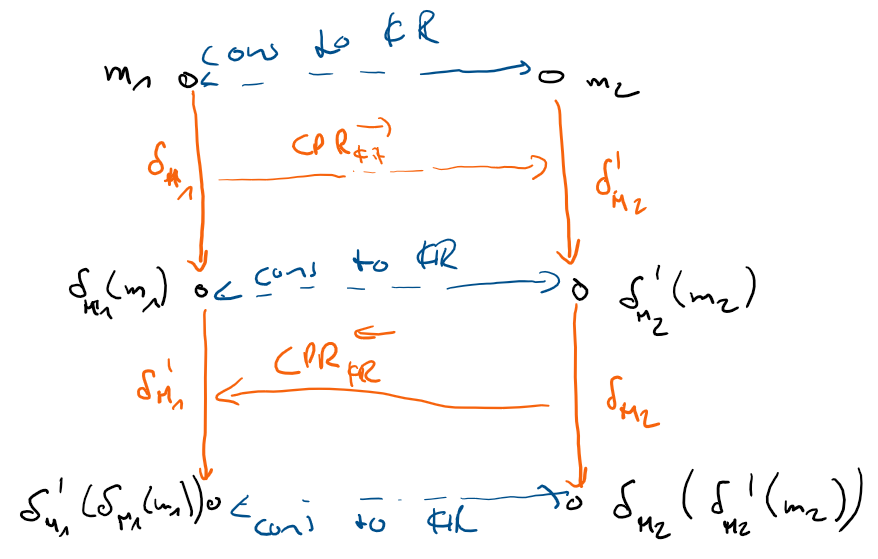
\includegraphics[width=0.8\textwidth]{figures/correctness/synchronization/sequencing_schema.png}
    \caption[Sequencing unidirectional consistency preservation rules]{Schema for sequencing unidirectional consistency preservation rules after concurrent changes. Circles denote model states, blue lines connect consistent models, and green lines with arrowheads denote the execution of changes or consistency preservation.}
    \label{fig:synchronization:sequencing_schema}
\end{figure}

\mnote{Changes affecting disjoint element sets}
The sequential application of original changes and execution of consistency preservation rules is depicted schematically in \autoref{fig:synchronization:sequencing_schema}.
It has two important properties. 
First, it ensures that all original changes are applied to the models and, second, it guarantees that the resulting models are consistent.
It is, however, only applicable in specific situations.
The optimal case, in which the approach is always applicable, is if $\consistencypreservationrule{\consistencyrelationset{CR}}^{\rightarrow}$ produces changes for the second model that affect a disjoint set of elements in $\consistencyrelationset{CR}$ compared to the original changes to the second model $\change{\metamodel{M}{2}}$.
If two changes affect completely disjoint sets of elements, they can obviously be consecutively applied.
It would then not even make a difference in which order they are applied.

\begin{figure}
    \centering
    \newcommand{\classwidth}{5em}
\newcommand{\objectwidth}{5em}
\newcommand{\hdistance}{19em}

\begin{tikzpicture}

\umlclassvarwidth{employee_class}{}{Employee}{
    name
}{\classwidth}
\umlclassvarwidth[, right=1.4*\hdistance of employee_class.north west, anchor=north]{resident_class}{}{Resident}{
    name
}{\classwidth}
\node[above=0.2em of employee_class.north, anchor=south] {$\metamodel{M}{1}$};
\node[above=0.2em of resident_class.north, anchor=south] {$\metamodel{M}{2}$};

\draw[directed consistency relation]
    (employee_class)
    --
    node[pos=0, below right] {$e$}
    node[pos=1, below left] {$r$}
    node[above] {$\consistencyrelation{CR}{ER} = \setted{\tupled{e,r} \mid \mathvariable{e.name} = \mathvariable{r.name.toLower}}$}
    node[below, align=center] {$\consistencyrelationset{CR} = \setted{\consistencyrelation{CR}{ER}, \consistencyrelation{CR}{ER}^T}$}
    (resident_class);

% FIRST SCENARIO
\coordinate (begin_first) at ([yshift=-0.2*\hdistance]employee_class.north west);
\draw[lightgray] (begin_first) -- (begin_first-|resident_class.east);

\umlobjectvarwidth[, below right=0.11*\hdistance and 0.35*\hdistance of begin_first, anchor=north]{employee_first}{}{: Employee}{
    name = "alice"
}{\objectwidth}
\umlobjectvarwidth[, right=0.85*\hdistance of employee_first.center, anchor=center]{resident_first}{}{: Resident}{
    name = "alice"
}{\objectwidth}
\umlobjectvarwidth[, below=0.2*\hdistance of resident_first.center, anchor=center]{resident2_first}{}{: Resident}{
    name = "Alice"
}{\objectwidth}
\node[above=0.2em of employee_first.north, anchor=south] {$\model{m}{1}$};
\node[above=0.2em of resident_first.north, anchor=south] {$\model{m}{2}$};

\draw[consistency execution]
    ([xshift=-0.2*\hdistance]employee_first.west)
    --
    node[above, align=center] {$\change{\metamodel{M}{1}}$}
    (employee_first.west);
\draw[consistency execution]
    ([yshift=0.5em]employee_first.east)
    --
    node[above] {$\change{\metamodel{M}{2}}' = \consistencypreservationrule{\consistencyrelationset{CR}}^{\rightarrow}$}
    ([yshift=0.5em]resident_first.west);
\draw[consistency execution]
    ([xshift=0.2*\hdistance]resident2_first.east)
    --
    node[above, align=center] {$\change{\metamodel{M}{2}}$}
    (resident2_first.east);
\draw[correspondence]
    ([yshift=-0.5em]employee_first.east)
    --
    node[below, pos=0.4] {consistent to $\consistencyrelationset{CR}$}
    ([yshift=-0.5em]resident_first.west);
\draw[correspondence]
    (employee_first.south)
    |-
    node[below, pos=0.75] {inconsistent to $\consistencyrelationset{CR}$}
    (resident2_first.west);
\coordinate (cross_first) at ([xshift=-0.05*\hdistance]resident2_first.west);
\draw[correspondence]
    (cross_first)
    |-
    ([yshift=-1em]resident_first.west);
\filldraw[consistency related element] (cross_first) circle (0.15em);

\end{tikzpicture}
    %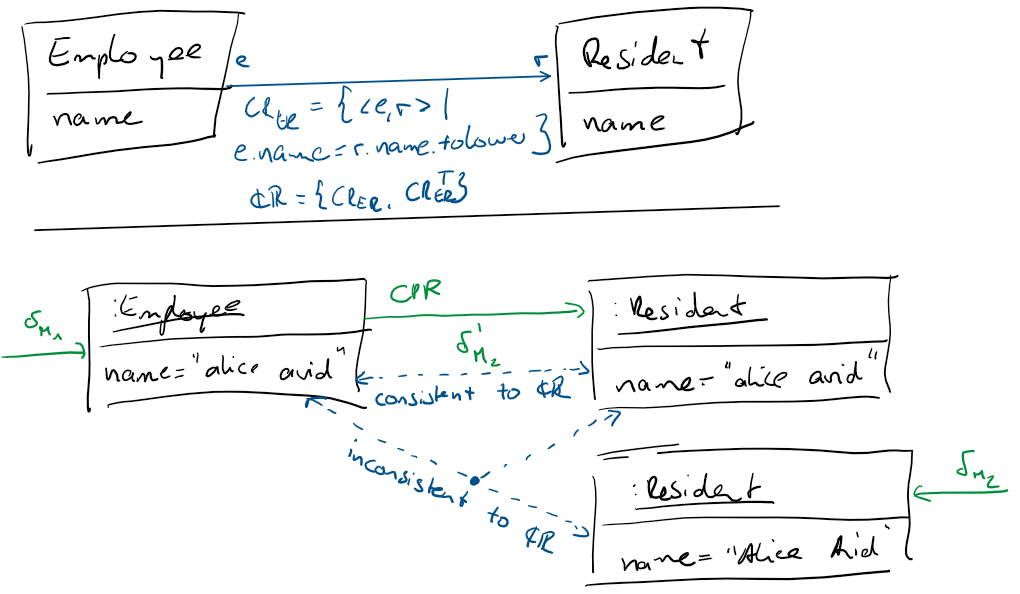
\includegraphics[width=0.9\textwidth]{figures/correctness/synchronization/non_transformability.png}
    \caption[Non-transformability in sequencing scenario]{Example for non-transformability when sequencing the application of unidirectional consistency preservation rules and concurrent changes.
    Blue lines without arrowheads connect elements that are \mbox{(in-)}consistent to $\consistencyrelationset{CR}$, and green lines with arrowheads indicate changes.}
    \label{fig:synchronization:non_transformability}
\end{figure}

\mnote{Issues when sequencing preservation rule application}
Unfortunately, the change $\change{\metamodel{M}{2}}'$ produced by $\consistencypreservationrule{\consistencyrelationset{CR}}^{\rightarrow}$ and the original one $\change{\metamodel{M}{2}}$ produced by other transformations do not necessarily affect disjoint sets of elements.
In that case, the two following problems can occur.
\begin{properdescription}
    \item[Non-Applicability:] The most obvious problem, which we have already discussed, is that the original change to the second model $\change{\metamodel{M}{2}}$ cannot be applied to the model changed by $\change{\metamodel{M}{2}}'$ as the result of $\consistencypreservationrule{\consistencyrelationset{CR}}^{\rightarrow}$. 
    This can, for example, happen when $\change{\metamodel{M}{2}}'$ removes an element that is affected by $\change{\metamodel{M}{2}}$.
    Since the element was changed in $\change{\metamodel{M}{2}}$, it is part of a condition element in another transformation that was executed before.
    As $\consistencypreservationrule{\consistencyrelationset{CR}}^{\rightarrow}$ removed that element, the condition element does no longer exist anyway, thus this removal has to be propagated back by the transformation that originally introduced the change $\change{\metamodel{M}{2}}$.
    In consequence, the modification in $\change{\metamodel{M}{2}}$ can simply be ignored.
    In the worst case, all elements affected by $\change{\metamodel{M}{2}}$ were removed by $\change{\metamodel{M}{2}}'$.
    Then, $\change{\metamodel{M}{2}}$ can be completely ignored, because all condition elements of the involved consistency relations were removed.
    Thus, we can always ensure that the changes, at least those that are still relevant, can still be applied.
    
    \item[Non-Transformability:] Even if the change $\change{\metamodel{M}{2}}$ can be applied to $\change{\metamodel{M}{2}}'(\model{m}{2})$, this does not guarantee that $\consistencypreservationrule{\consistencyrelationset{CR}}^{\leftarrow}$ is able to process the given change.
    In fact, this requirement applies to all changes, even including original user changes, but there are special circumstances in this situation that make the transformation prone to not being able to transform the changes.
    Whenever $\change{\metamodel{M}{2}}'$ adds condition elements that were already added by $\change{\metamodel{M}{2}}$, their concatenation can lead to a duplication of those elements.
    Consider the scenario depicted in \autoref{fig:synchronization:non_transformability} with consistency relations $\consistencyrelationset{CR} = \setted{\consistencyrelation{CR}{ER}, \consistencyrelation{CR}{ER}^T}$. 
    An employee \enquote{alice} is added by the original change to $\model{m}{1}$.
    The consistency preservation rule then generates an appropriate resident with the same name to fulfill the consistency relation.
    The original change to $\model{m}{2}$ adds a resident \enquote{Alice}, which was generated by another transformation, e.g., the one that created an appropriate person and changed the capitalization of the name.
    Applying this original change leads to two residents with different name capitalizations.
    Now it is impossible for $\consistencypreservationrule{\consistencyrelationset{CR}}^{\leftarrow}$ to generate a change $\change{\metamodel{M}{1}}'$ for the first model to restore consistency. The employee corresponds to both residents, as both fulfill the constraint of the consistency relation. 
    But there is no additional employee that could be added to achieve a unique mapping between corresponding elements.
    A synchronizing transformation would have been able to produce a consistent result by considering both original changes at once and then simply not performing any additional changes, as the originally added resident is already consistent to the originally added employee.
    In consequence, if the unidirectional consistency preservation rule had known that the resident was already added, it would not have performed any changes.
\end{properdescription}

\mnote{Non-transformable changes of users unavoidable}
As remarked before, the situation that certain changes cannot be processed by the consistency preservation rules cannot be avoided. 
If the user had added the second resident in the previous scenario, there would have also been no possibility for the consistency preservation rule to generate changes that restore consistency.
The difference is, however, that in this case it is fine that no result is found.
In case of the scenario discussed above, the original changes could have been reasonably processed to a consistent result if the unidirectional consistency preservation rule would have considered that there was already a change that restored consistency.

\mnote{Necessity to process inconsistent inputs}
In consequence, it is inevitable that consistency preservation rules need to be able to deal with the situation that the target model was already modified, such that the given models are not initially consistent.
This is necessary to reflect the changes that have already been made and to integrate them into consistency preservation.
In consequence, we finally have to relax our requirements for the input of consistency preservation rules to be able to consider the changes to both models.
This means that we need to make further requirements to the preservation rules, because we do not yet assume the consistency preservation rules to produce results for inputs that are not consistent.
We have already given examples for scenarios in which it is not possible to restore consistency by one unidirectional consistency preservation rule after changes in both models.

\mnote{Relaxed notion affecting number of executions}
Before we define a precise notion of further requirements to consistency preservation rules that accept inconsistent inputs, we first discuss how often it may be necessary to execute both consistency preservation rules to restore consistency, as this directly affects the requirements we have to define.


%%%
%%% NON-TERMINATION
%%%
\subsection{Execution Bounds}
\label{chap:synchronization:combination:bounds}

\mnote{Unidirectional preservation rules cannot always be correct}
Correctness of unidirectional consistency preservation rules ensures that after executing such a rule the resulting models are consistent.
It is easy to see that this correctness notion cannot be fulfilled for certain sets of consistency relation sets.
This is exemplified at the artificial scenario depicted in \autoref{fig:synchronization:multiple_unidirectional_execution}.
We consider two consistency relations $\consistencyrelation{CR}{1}$ and $\consistencyrelation{CR}{2}$ and their transposed relations, i.e., $\consistencyrelationset{CR} = \setted{\consistencyrelation{CR}{1}, \consistencyrelation{CR}{1}^T, \consistencyrelation{CR}{2}, \consistencyrelation{CR}{2}^T}$.
$\consistencyrelation{CR}{1}$ requires that for each \modelelement{A} an instance of \modelelement{B} exists that has the same value of $i$ incremented by $1$.
The only exception is that if $i$ in \modelelement{A} is $4$ (or any other arbitrary value), then no corresponding element \modelelement{B} is required.
$\consistencyrelation{CR}{2}$ requires that for each \modelelement{A} an instance of \modelelement{B} exists, which has the same value of $i$.
We want to define a bidirectional transformation of two unidirectional consistency preservation rules $\consistencypreservationrule{\consistencyrelationset{CR}}^{\rightarrow}$ for propagating changes in models with instances of \modelelement{A} to one with instances of \modelelement{B} and $\consistencypreservationrule{\consistencyrelationset{CR}}^{\leftarrow}$ to propagate changes in the opposite direction. 

\begin{figure}
    \centering
    \newcommand{\hdistance}{24em}
\newcommand{\vdistance}{9.5em}
\newcommand{\classwidth}{2.5em}

\begin{tikzpicture}[
    relation/.style={consistency relation, font=\footnotesize}
]

\umlclassvarwidth{A}{}{A}{
i
}{\classwidth}

\umlclassvarwidth[,right=\hdistance of A.north, anchor=north]{B}{}{B}{
i
}{\classwidth}

% CONSISTENCY RELATIONS
\draw[relation] 
    ([yshift=0.3em]A.east)
    --
    node[pos=0, above right] {$a$}
    node[pos=1, above left] {$b$}
    node[below, align=left] {
    $\consistencyrelation{CR}{1} = \setted{\tupled{a,b} \mid a.i, b.i \ge 0 \land b.i = a.i + 1 \neq 5}$\\
    $\consistencyrelation{CR}{2} = \setted{\tupled{a,b} \mid a.i = b.i}$
    }
    ([yshift=0.3em]B.west);

\end{tikzpicture}
    %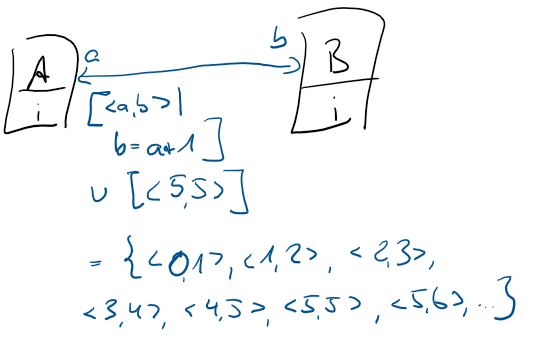
\includegraphics[width=0.7\textwidth]{figures/correctness/synchronization/multiple_unidirectional_execution.png}
    \caption[Multiple execution of consistency preservation rules]{Two consistency relations requiring multiple executions of unidirectional consistency preservation rules to find a consistent result.}
    \label{fig:synchronization:multiple_unidirectional_execution}
\end{figure}

\mnote{Example scenario}
Consider the following scenario: If an \modelelement{A} with $i = 0$ is added to an empty model, $\consistencypreservationrule{\consistencyrelationset{CR}}^{\rightarrow}$ cannot perform any changes in an (also empty) model with instances of \modelelement{B} that restore consistency.
Because of $\consistencyrelation{CR}{1}$, a \modelelement{B} with $i = 1$ has to be created, and because of $\consistencyrelation{CR}{2}$, a \modelelement{B} with $i = 0$ has to be created.
While this also fulfills $\consistencyrelation{CR}{1}^T$, the existence of \modelelement{B} with $i = 1$ requires the existence of an \modelelement{A} with $i = 1$ due to $\consistencyrelation{CR}{2}^T$.
Since $\consistencypreservationrule{\consistencyrelationset{CR}}^{\rightarrow}$ cannot modify the model with instances of \modelelement{A}, it is impossible for $\consistencypreservationrule{\consistencyrelationset{CR}}^{\rightarrow}$ to restore consistency in that case.

\mnote{Multiple executions leading to consistent result}
Allowing the consistency preservation rules to react to each other multiple times can, however, lead to a consistent result.
If $\consistencypreservationrule{\consistencyrelationset{CR}}^{\leftarrow}$ adds an \modelelement{A} with $i = 1$ in response to the previous execution of $\consistencypreservationrule{\consistencyrelationset{CR}}^{\rightarrow}$, all consistency relations except $\consistencyrelation{CR}{1}$ are fulfilled.
$\consistencypreservationrule{\consistencyrelationset{CR}}^{\rightarrow}$ can then create a \modelelement{B} with $i = 2$, which is iteratively processed by $\consistencypreservationrule{\consistencyrelationset{CR}}^{\leftarrow}$.
This process terminates as soon as $\consistencypreservationrule{\consistencyrelationset{CR}}^{\leftarrow}$ adds an \modelelement{A} with $i = 4$, as then $\consistencyrelation{CR}{1}$ is also fulfilled, because it does not require a corresponding \modelelement{B} for an \modelelement{A} with $i = 4$.

\mnote{Arbitrary high number of necessary executions}
We have seen that it is possible to execute unidirectional consistency preservation rules multiple times to achieve a consistent state and that it is not always possible to ensure consistency with only one execution of such a rule.
In fact, the number of necessary executions of consistency preservation rules can be arbitrarily high.
The value of $5$ in $\consistencyrelation{CR}{1}$ of the example can be exchanged by any value requiring an arbitrary high number of executions.
We may only circumvent this by requiring that $\consistencypreservationrule{\consistencyrelationset{CR}}^{\rightarrow}$ must perform changes such that $\consistencypreservationrule{\consistencyrelationset{CR}}^{\leftarrow}$ can then restore consistency with a single execution.
In our scenario, this would mean that $\consistencypreservationrule{\consistencyrelationset{CR}}^{\rightarrow}$ adds all instances of \modelelement{B} with $i \leq 4$.
Anyway, such a behavior requires a relaxation of the correctness requirement for consistency preservation rules, because the execution of $\consistencypreservationrule{\consistencyrelationset{CR}}^{\rightarrow}$ can never result in a consistent state.

\mnote{Preservation rules complete partial condition elements}
Additionally, it may be desired that elements of a consistency relation are created by a consistency preservation rule, although a condition element was only created partially so far.
In that case, the partial condition element has to be completed in one model in addition to the creation of the corresponding condition element in the other model.
Thus, changes in both models are required, which can only be achieved by executing both consistency preservation rules and accepting that executing the first one does not result in consistent models.
An example for such a scenario could be the consistency relation between a component in the \gls{PCM} and its realization as a package and a class in Java.
It may be desired that a package at a specific place, e.g., within a \enquote{components} package, or with a specific name, e.g., containing \enquote{Component}, in the Java code is identified as a component.
Creating such a package shall then lead to the creation of a component in the the \gls{PCM} model as well as of the implementation class in Java.
In that case, there is no complete condition element created in Java, because this would also require the existence of an appropriate class.
If the elements shall still be created, both models have to be changed.
Thus, the first consistency preservation rule introduces the \gls{PCM} component, which introduces an inconsistency between the models, as the corresponding Java class is missing.
This is then corrected by the consistency preservation rule in opposite direction adding the implementation class.

\mnote{Necessity of termination guarantee}
Finally, it is questionable whether such scenarios should be considered in the formal framework or if it should be up to a developer to implement such a scenario without having specific guarantees regarding termination of the consistency preservation rules or regarding consistency of the models after executing the rules a specific number of times.
Since we need to relax the requirement of consistency preservation rules to always produce consistent results after one execution in the synchronization scenario where both models have been modified, we will allow the consistency preservation rules to be executed more than once anyway.
Regarding the example in \autoref{fig:synchronization:multiple_unidirectional_execution}, if we started with an \modelelement{A} with $i = 6$ and let the consistency preservation rules operate as discussed above, i.e., always adding the elements with $i$ incremented by one, this process would never terminate.
We thus need to ensure that such an execution terminates.
Since the consistency preservation rules depend on each other, this will, however, be a property of the bidirectional transformation rather than the individual consistency preservation rule.


\subsection{Necessity for Synchronization Extension}

\mnote{Processing inconsistent input models}
In the previous subsections, we have discussed that after changes to two models, these changes and the ones produced by consistency preservation rules that restore consistency between these models cannot be sequenced in a way such that we receive consistent models in all cases the consistency preservation rules are able to handle.
We especially found that it is necessary for a unidirectional consistency preservation rule to consider the changes made to the model it is supposed to modify.
Thus, we need to enable consistency preservation rules to deal with the situation that the input models are inconsistent.
In our current definition, no behavior of a consistency preservation rule and the encapsulating bidirectional transformation for such a situation is defined.
Thus, we discuss an appropriate extension of bidirectional transformations that support this scenario of synchronization in the following section.

\mnote{Guaranteeing termination}
Additionally, we found that consistency preservation rules may need to be executed multiple times.
This is obviously necessary to make bidirectional transformations synchronizing, as they need to be able to change both models after both of them may have been modified.
Therefore, we consider how we can achieve execution bounds, such that the termination of multiple executions of the consistency preservation rules of a bidirectional transformation is guaranteed.



%%%%
%%%% VERSCHIEDENE VERSUCHE FÜR STRATEGIEN ZUR KOMBINATION VON CPRS
%%%%

% \subsection{Consideration at Condition Element Level}
% % CONSIDERATIONS DO NOT WORK PROPERLY
% \begin{itemize}
%     \item Unidirectional synchronizing: correct if applied to changes d1 to m1, but produces changes d2' that can be applied to d2(m2) as well, and vice versa produces changes d1' for changes d2 to model m2 that can be applied to d1(m1) as well. (Property: Sequentializability, produced changes can handle arbitrary other changes added before)
%     \item For each condition element in d1(m1), i.e., each element for which a consistency relation applies, and for each condition element in d2'(m2), we find exactly one corresponding element in the other model (this is what correctness means). Additionally, in d2'(d2(m2)) $\cap$ d2'(m2), i.e., those elements that are not affected by d2, we also find corresponding 
    
%     \item Take all condition elements in m1 and m2. Take all those for which still only one corresponding condition element exists between m1 and d2(m2), i.e., all the ones not affected by d2. For all of them present in d1(m1) and d2'(d2(m2)), there is still exactly one corresponding condition element. For the ones in d1(m1), which were not in m1, there is a corresponding element in d2'(d2(m2)) and for the ones in d2'(m2), which are also present in d2'(d2(m2)), there is one in d1(m1).
%     \item What if d2'(d2(m2)) produces a new condition element that was not present in m2 and d2(m2) and d2'(m2)? We need to show that this cannot occur?
%     \item Non-synchronizing: d1 and d2 may induce violations of consistency relations. d1' and d2' restore fulfillment of these consistency relations. We consider how consistency relations can be violated when we put d2 in front of d2' and d1 in front of d1' other than in the case when its applied directly.
% \end{itemize}


% \subsection{Versuch über ursächliche Condition Element Änderungen zu unterscheiden}
% Fälle:
% 1. Condition Element wird neu erzeugt
% 2. Condition Element wird geändert, sodass nun ein anderes Element der gleichen Condition vorhanden ist
% 3. Condition Element wird gelöscht
% Es können bei einem Change mehrere davon bzgl. verschiedener Conditions auftreten (also bzgl. verschiedene Consistency Relations)

% Fall 1: Die Vereinigung der Condition Elements aus d2(m2) und d2'(m2) ist gleich derer in d2'(d2(m2)). Somit wird durch die Kombination kein neues Condition Element eingeführt, für das Konsistenz hergestellt werden müsste.

% Fall 2: Die Vereinigung der Condition Elements aus d2(m2) und d2'(m2) ist ungleich derer in d2'(d2(m2)). Somit wird durch die Kombination ein neues Condition Element eingeführt, für das Konsistenz hergestellt werden müsste.

% NEUE STORY:

% Allgemeine Betrachtung von Änderungen: Es geht immer darum, dass Condition Elemente geändert/gelöscht/hinzugefügt wurden und die CPR entsprechend reagieren muss, um das Vorhandensein einer entsprechenden Witness-Struktur zu garantieren. Dabei können entsprechend folgende Fälle auftreten:
% 1. Änderungen führen dazu, dass ein neues Condition Element im Modell existiert, dass zuvor nicht vorhanden war.
% 2. Änderungen führen dazu, dass Elemente eines bereits vorhandenes Condition Elementes geändert werden und dadurch ein andere Condition Element derselben Condition instanziieren.
% 3. Änderungen führen dazu, dass ein vorher existierendes Condition Element nicht mehr im Modell auftaucht.

% Es gibt hierzu drei entsprechende Reaktionen der CPR:
% 1. Im anderen Modell werden, falls nicht vorhanden, entsprechende Elemente erzeugt, um für das neue Condition Element ein eindeutiges korrespondierendes Condition Element zu erzeugen und somit eine Witness-Struktur aufzubauen. (Erzeugungs-Propagation)
% 2. Das gem. Witness-Struktur korrespondierende Condition Element im anderen Modell wird so angepasst, dass wieder eine valide Witness-Struktur entsteht. (Änderungs-Propagation)
% 3. In dem anderen Modell werden die Elemente des korrespondierenden Condition Elementes entfernt (oder zumindest Teile davon), sodass entsprechend der Konsistenzregeln keine weiteren Elemente vorhanden sein müssen, d.h. wieder eine valide Witness-Struktur vorhanden ist.

% % DIE FOLGENDEN ZWEI PARAGRAPHEN SIND NUN BEI DER STRIKTEN SEQUENTIALISIERUNG
% Wenn wir die unidirektionalen CPR sequentialisieren (also erst d2' erzeugen, dann d2 darauf anwenden), kann es sein, dass d2'(m2) Änderungen an Condition Elements in m2 vornimmt oder neue hinzufügt, um Konsistenz wiederherzustellen, die ebenfalls von d2 eingefügt werden, sodass es nicht mehr möglich ist, durch die rückwärtige CPR Änderungen vorzunehmen, die eine valide Witness-Struktur induzieren.
% Z.B. könnte d2'(m2) einen Resident hinzufügen, der bereits durch d2 eingefügt wurde (weil er über einen andere Pfad erstellt wurde, siehe \autoref{fig:synchronization:duplicate_creation_example}). Wird nun d2 auf d2'(m2) angewendet, würde ggf. in einem Container, in dem die Residents gespeichert werden, zwei Residents mit gleichem Namen eingefügt. Für diese kann aber keine Änderung in m1 (sei es das Employee-Modell) erzeugt werden, durch die eine valide Witness-Struktur entsteht. Das Einfügen eines zweiten Employee mit dem gleichen Namen führt dazu, dass jeder Employee und jeder Resident zu zwei Residents bzw. Employees korrespondiert, was keine eindeutige Witness-Struktur induziert.
% Um dies zu vermeiden, müssen die CPR sicherstellen, dass in den Änderungen am anderen Modell nicht bereits entsprechende Condition Elements erzeugt wurden.
% Alle anderen Änderungen sind unproblematisch, da Änderungen die d2 an bestehenden Condition Elements, die nicht zu neuen Condition Elements führen, durchführt mittels 2->1 propagiert werden können, indem die Condition Elements in m1 angepasst werden.

% Insgesamt ist die Situation die gleiche, als würde ein Nutzer eine entsprechende Änderung machen. Auch er kann natürlich einen zweiten Resident mit demselben Namen einführen. Hier würde die CPR selbstverständlich fehlschlagen. Während das für Nutzeränderungen erwünscht ist, da die doppelte Erzeugung desselben Elementes hier schon vom Nutzer durchgeführt wurde und für einen entsprechende Nutzeränderung kein konsistentes Modell generiert werden kann, ist dies innerhalb des Transformationsnetwerkes unerwünscht, da die CPR natürlich eine konsistente Modellmenge finden können und die doppelte Erzeugung lediglich daher kommt, dass die Transformationen nicht, wie verlangt, synchronisieren sind. In letztem Fall wäre sichergestellt, dass nach entsprechenden Änderungen an beiden Modellen (also Erzeugung von Employee in einem, Erzeugung des passenden Resident im anderen) keine Änderungen gemacht werden, da bereits eine passende Witness-Struktur vorhanden ist.
% Die unidirektionalen CPR schaffen das jedoch nicht, da Ihnen die entsprechende Information fehlt.


% \subsection{Erster Versuch zur Partiellen Konsistenz}
% % DIE FOLGENDEN PARAGRAPHEN SIND IN DER PARTIELLEN KONSISTENZ AUFGEGANGEN, NUR DAS PARTIELLE KONSISTENZ ÜBER MODELLE UND NICHT ÜBER CPR DEFINIERT IST
% Was kann nun passieren, wenn wir die CPR mit dem modifizierten Ziel-Modell aufrufen?
% Wir müssen Def anpassen, da es nun nicht mehr reicht, wenn CPR für konsistente Eingabe korrekt ist.

% m1 und d2(m2) sind ja immer noch partiell konsistent. Wir betrachten für jedes Konsistenzrelation alle condition elements in m1 und d2(m2).
% Diejenigen, für die es ein eindeutiges korrespondierendes Element gibt, also eine maximale Menge (es gibt keine Menge, von der sie eine Teilmenge ist) für die es eine Witness-Struktur gibt, und die immer noch in d1(m1) bzw. d2'(d2(m2)) vorkommen, muss es auch darin ein eindeutiges korrespondierendes Element geben.
% Außerdem muss für alle Condition Elements in d1(m1) $\setminus$ m1 und in d2'(d2(m2)) $\setminus$ d2(m2) ein eindeutiges korrespondierendes Element existieren.
% Dies ist bereits dadurch sichergestellt, dass ja die CPR immer auf das Erzeugen/Ändern/Löschen eines Condition Elementes reagieren, d.h. für die Element ein d1(m1) $\setminus$ m1 stellt es Konsistenz sicher und für d2'(d2(m2)) auch, da es sonst eine neue Inkonsistenz induzieren würde.
% D.h. nur für Elemente, die vorher nicht konsistent waren, ist keine Konsistenz verlangt.

% Property: Always-preserving
% CPR erhält Konsistenz für solche Elemente, die vorher konsistent waren. D.h. wenn es eine Witness-Struktur für eine Teilmenge der Modelle gibt, dann gibt es sie auch nach den Änderungen (also in d1(m1) und d2'(d2(m2))) für dieselben Teilmengen (bzw. das was noch davon da ist), egal ob die Modelle vorher konsistent waren oder nicht. (es ist schwer diese Eigenschaft für Transformationen zu zeigen, aber die empirische Evaluation zeigt, dass die Annahme dort zumindest gilt)

% Property: Delta-Correcting
% CPR stellt Konsistenz für solche Elemente her, die durch das Delta im Quellmodell und Zielmodell hinzugefügt werden. Also für alle Condition Elements in d1(m1) $\setminus$ m1 und in d2'(d2(m2)) $\setminus$ d2(m2) muss ein eindeutiges korrespondierendes Element existieren.

% \subsection{Zweiter Ansatz zur partiellen Konsistenz auf Condition Element Level}
% Wir fordert für alle Condition Elements in d1(m1) und alle in m1, die noch immer in d1(m1) vorkommen, dass sie wieder ein eindeutiges korrespondierendes in d2'(d2(m2)) haben, wenn sie in m1 vorhanden waren und dort ein korrespondierendes in d2(m2) hatten.
% Fallunterscheidung:
% * Sie waren in m1 vorhanden, aber in d1(m1) nicht mehr: Dann wurden sie geändert. Wurde das korrespondierende Element in d2(m2) nicht gegenüber m2 geändert, muss es mit d2'(d2(m2)) von CPRr angepasst werden, da sonst auch ohne d2(m2) CPRr die Änderung nicht vorgenommen hätte und damit nicht korrekt wäre. Wurde das Element in d2(m2) gegenüber m2 geändert, so kümmert sich CPRl noch um diese Änderung. \todo{Das können wir nicht transitiv so machen}
% * \dots


% \subsection{Co-occurring Changes to Corresponding Elements}
% Two problem cases: 
% 1. Both d1 and d2 affect corresponding condition elements (otherwise show that it is unproblematic); 
% 2. d2'(d2(m2)) introduced new condition elements that were neither present in m2, nor in d2'(m2), nor d2(m2), so they are neither consistent due to correctness of forward preservation rule, nor processed by backward preservation rule.
% \begin{itemize}
%     \item If d1 affects a condition element (be it a change of an existing, the creation of a new one or the removal of an old one), then preservation needs to generate a d2' that updates/creates/removes the corresponding condition elements appropriately, such that even elements that are potentially part of another condition element, fulfill consistency (due to correctness). If d2 does not affect any of the corresponding or other changes elements, everything is fine, because then we can simply sequence changes.
%     \item 
% \end{itemize}
    
% Szenarien:
% Auf jeder Seite wurde ein Condition Element modifiziert.
% 1. 1->2 und 2->1 ändern jeweils Elemente aus komplett disjunkten Condition Elements: Witness-Struktur ergibt sich aus alter Witness-Struktur und für entfernen von Element und korrespondierendem das Entfernen der Korrespondenz, Hinzufügen und Element und korrespondierendem das Hinzufügen der Korrespondenz, sowie Ändern eines Condition Elementes zu einem anderen das Ändern der entsprechenden Korrespondenz.
% 2. 1->2 (resp.~2->1) fügen durch Änderungen neues Condition Element ein: Sind per Korrektheit verpflichtet das richtig aufzulösen
% 3. \dots

\section{Synchronizing Bidirectional Transformations}

\mnote{Extend consistency preservation rules to accept models that are not consistent}
In the following, we discuss how we can extend bidirectional transformations and especially their unidirectional consistency preservation rules such that they are able to deal with the situation that both models may have been modified.
To achieve this, we extend consistency preservation rules such that they also accept models that are not initially consistent.
We can then not require them to restore consistency between the models with a single execution anymore.
Instead, we define a notion of \emph{partial consistency}, which allows us to specify how the execution of consistency preservation rules has to improve partial consistency.
We derive requirements to the transformations and finally show that transformations fulfilling these requirements terminate consistently.


\subsection{Partial Consistency of Models}

\mnote{Changed models still fulfill some kind of partial consistency notion}
Given two models $\model{m}{1}$ and $\model{m}{2}$ and changes $\change{\metamodel{M}{1}}$ and $\change{\metamodel{M}{2}}$ to each of them, a unidirectional consistency preservation rule $\consistencypreservationrule{\consistencyrelationset{CR}}^{\rightarrow}$ needs to accept and process the change in one model, be it $\change{\metamodel{M}{1}}$ without loss of generality, and receive the unchanged model $\model{m}{1}$ as well as the changed second model $\change{\metamodel{M}{2}}(\model{m}{2})$.
We discussed the necessity to process the changed second model in the previous section.
Whereas $\model{m}{1}$ and $\model{m}{2}$ are consistent, $\model{m}{1}$ and $\change{\metamodel{M}{2}}(\model{m}{2})$ may not.
In consequence, $\consistencypreservationrule{\consistencyrelationset{CR}}^{\rightarrow}$, even if correct according to \autoref{def:unidirectionalconsistencypreservationrulecorrectness}, cannot guarantee that applying the delivered change delivers consistent models.
$\model{m}{1}$ and $\change{\metamodel{M}{2}}(\model{m}{2})$ will, however, usually still fulfill some kind of partial consistency notion.
Depending on the complexity of $\change{\metamodel{M}{2}}$ large parts of the models will still fulfill some kind of consistency notion.

\mnote{Two options to define partial consistency}
Such a notion of partial consistency may be defined in two different ways.
First, we may say that two models only fulfill the consistency relations partially.
Second, we may say that only extracts of two models fulfill the consistency relations.

\mnote{Partial consistency as fulfilling subsets of consistency relations}
In the first option, we consider that the given models are only consistent to a subset of the given consistency relations.
There may, however, be only a single element in the models that leads to the violation of all consistency relations.
Thus, we would call the models completely inconsistent just because of a single element.
To circumvent hat, we would need to define a notion of partial consistency relations, which allows us to define that models are consistent to parts of consistency relations.
Such a notion would have to be defined at the level of consistency relation pairs and their condition elements within the consistency relations.
It would, however, not make sense to consider subsets of consistency relations, i.e., only a subset of their consistency relation pairs, because when analyzing consistency of two models those consistency relation pairs are not independent.
If two models contain the condition elements of one consistency relation pair, this may prevent the, from containing the condition elements of another consistency relation pair, because in \autoref{def:consistency} we require a unique mapping between condition elements in terms of witness structure.
If models are consistent to a consistency relation in which we removed one (or more) consistency relation pairs, this does not give any reasonable indication on how the models violate consistency.
This may be due to the reason that an element is missing in the models or that an additional element prevents from finding a witness structure.
It does, however, not mean that adding a missing element or removing the additional element ensures that a proper witness structure can be found, because these elements may still be relevant for other consistency relation pairs in the witness structure.
These interdependencies of consistency relation pairs are the reason why consistency to partial consistency relations does not provide insights on the reasons for models being inconsistent.
Thus, we do not consider this as our notion for partial consistency.

\mnote{Partial consistency as parts of the models fulfilling consistency relations}
In the second option, we consider that only parts of the given models are consistent to all given consistency relations.
In addition to the missing ability of the first option to give reasonable insights on inconsistencies, this, intuitively, is a more reasonable notion, because it explicitly defines that parts of the models are consistent, whereas other parts of them are not.
We thus define partial consistency as models having subsets that are actually consistent.
To identify how far models are partially consistent, we also define an according metric.
It is based on the idea to find maximal subsets of the models that are consistent.

\begin{definition}[Partial Consistency] \label{def:partialconsistency}
    Let $\consistencyrelationset{CR}$ be a set of consistency relations.

    Given two models $\model{m}{1} \in \metamodelinstanceset{M}{1}$ and $\model{m}{2} \in \metamodelinstanceset{M}{2}$, we define their \emph{maximal consistent subsets} $\model{m}{1}^p \in \metamodelinstanceset{M}{1}$ and $\model{m}{2}^p \in \metamodelinstanceset{M}{2}$ with regards to $\consistencyrelationset{CR}$ as the subsets of $\model{m}{1}$ and $\model{m}{2}$ that are consistent and larger than all other consistent subsets:
    \begin{align*}
        & 
        \tupled{\model{m}{1}^p, \model{m}{2}^p} \consistenttomath \consistencyrelationset{CR} \land
        \model{m}{1}^p \subseteq \model{m}{1} \land \model{m}{2}^p \subseteq \model{m}{2}  \\
        & \formulaskip
        \land \forall \model{m}{1}^{p'} \in \metamodelinstanceset{M}{1}, \model{m}{2}^{p'} \in \metamodelinstanceset{M}{2} : \\
        & \formulaskip\formulaskip
        \bigl(\model{m}{1}^{p'} \subseteq \model{m}{1} \land \model{m}{2}^{p'} \subseteq \model{m}{2} 
        \land \tupled{\model{m}{1}^{p'}, \model{m}{2}^{p'}} \consistenttomath \consistencyrelationset{CR} \\
        & \formulaskip\formulaskip
        \Rightarrow 
        \abs{\model{m}{1}^{p'}} + \abs{\model{m}{2}^{p'}} \leq \abs{\model{m}{1}^{p}} + \abs{\model{m}{2}^{p}} \bigr)
    \end{align*}
    We define partial consistency of two models with respect to $\consistencyrelationset{CR}$ as the ratio between the size of the maximal consistent subsets and the size of the models in $\function{cons}_{\consistencyrelationset{CR}}$:
    \begin{align*}
        \function{cons}_{\consistencyrelationset{CR}}: \; 
        & (\metamodelinstanceset{M}{1}, \metamodelinstanceset{M}{2}) \rightarrow [0,1] \\
        & 
        (\model{m}{1}, \model{m}{2}) \mapsto \frac{\abs{\model{m}{1}^{p}} + \abs{\model{m}{2}^{p}}}{\abs{\model{m}{1}} + \abs{\model{m}{2}}}
    \end{align*}
    % with:
    % \begin{align*}
    %     & 
    %     \exists \model{m}{1}^p \in \metamodelinstanceset{M}{1}, \model{m}{2}^p \in \metamodelinstanceset{M}{2} : \\
    %     & \formulaskip
    %     \tupled{\model{m}{1}^p, \model{m}{2}^p} \consistenttomath \consistencyrelationset{CR} \land
    %     \model{m}{1}^p \subseteq \model{m}{1} \land \model{m}{2}^p \subseteq \model{m}{2} : \\
    %     & \formulaskip
    %     \land \forall \model{m}{1}^{p'} \in \metamodelinstanceset{M}{1}, \model{m}{2}^{p'} \in \metamodelinstanceset{M}{2} : \\
    %     & \formulaskip\formulaskip
    %     \bigl(\model{m}{1}^{p'} \subseteq \model{m}{1} \land \model{m}{2}^{p'} \subseteq \model{m}{2} 
    %     \land \tupled{\model{m}{1}^{p'}, \model{m}{2}^{p'}} \consistenttomath \consistencyrelationset{CR} \\
    %     & \formulaskip\formulaskip
    %     \Rightarrow 
    %     \abs{\model{m}{1}^{p'}} + \abs{\model{m}{2}^{p'}} \leq \abs{\model{m}{1}^{p}} + \abs{\model{m}{2}^{p}} \bigr) \\
    %     &\formulaskip
    %     \land \function{cons}_{\consistencyrelationset{CR}}(\model{m}{1}, \model{m}{2}) = \abs{\model{m}{1}^{p}} + \abs{\model{m}{2}^{p}}
    % \end{align*}
\end{definition}

\mnote{Partial consistency can always be calculated}
Such maximal consistent subsets do always exist.
In the extreme case, when models are not consistent in any way, it is $\model{m}{1}^p = \model{m}{2}^p = \emptyset$, because empty models are always consistent by definition.
In that case, partial consistency of the models is $0$, whereas in cases when models are actually consistent the maximal consistent subsets are the models themselves, which is why partial consistency is $1$.

% \paragraph{Partielle Konsistenz}
% Gegeben m1, d2(m2) und d1.
% d1(m1) und d2(m2) sind partiell konsistent, d.h. es gibt Teilmengen d1(m1)p und d2(m2)p, für die alle Konsistenzrelationen erfüllt sind.
% Dies kann für mehrere Teilmengen gelten, wir betrachten die, die zusammen maximal groß sind, d.h. |d1(m1)p| + d2(m2)p| > |d1(m1)p'| + d2(m2)p'| für beliebige andere Teilmenge, die konsistent sind.
% TODO: Metrik definieren für partielle Konsistenz. Dann können nämlich einfach sagen, dass sich die partielle Konsistenz erhöhen muss (indem entweder die Modelle kleiner werden oder die konsistenten Teile größer)


\subsection{Transformations for Partially Consistent Models}
\label{chap:synchronization:bidirectional:transformations}

%\todo{Start section again without discussion the starting case for synchronization, but the general case of having partially consistent models. Then later apply it to the starting case for synchronization. Szenario ist, dass wir zwei Modelle reinkriegen (potentiell inkonsistent) und Änderungen an einem davon. Falls das zweite auch geändert wurde, diskutieren wir später, wie wir das noch reinkriegen (indem wir das Delta auf das zweite Modell anwenden und dann die Ausführung der Rückrichtung darauf anwenden).}

\mnote{Multiple executions of consistency preservation rules to resolve partial inconsistencies}
Before we consider the case that two models have been modified and need to be synchronized, we start with the case that of two initially consistent models one has been changed.
We then extend that scenario to the case when both models have been changed.
We use the notion of partial consistency to define that the given models are initially partially consistent and how this partial consistency improves by executing the bidirectional transformation.
As discussed in \autoref{chap:synchronization:combination:bounds}, it may be necessary to execute the consistency preservation rules multiple times to achieve a consistent state, producing several intermediate changes that generate partially consistent models.

\mnote{Execution steps of transformations apply both consistency preservation rules once}
In the following, we derive the properties a bidirectional transformation has to fulfill to eventually return models that are consistent if applied repeatedly.
They are based on the idea that each execution has to improve partial consistency of the given models.
Since a single consistency preservation rule may not be able to improve partial consistency in every case, we always consider the combination of both preservation rules of a bidirectional transformation and require that property from them.
Therefore, we define the notion of a \emph{bidirectional transformation execution step}, which is composed of a single execution of both unidirectional consistency preservation rules.
%This is necessary, because a single consistency preservation rule may not be able to improve partial consistency, whereas at least one of them should be, thus executing both may always lead to an improvement.
%Consider the case that a change was only performed to $\model{m}{2}$, then $\consistencypreservationrule{\consistencyrelationset{CR}}^{\rightarrow}$ cannot produce any reasonable changes in $\model{m}{2}$ to restore consistency.

\begin{definition}[Bidirectional Transformation Execution Step]
    Let $\transformation{T} = \tupled{\consistencyrelationset{CR}, \consistencypreservationrule{\consistencyrelationset{CR}}^{\rightarrow}, \consistencypreservationrule{\consistencyrelationset{CR}}^{\leftarrow}}$ be a bidirectional transformation for metamodels $\metamodel{M}{1}$ and $\metamodel{M}{2}$.
    An \emph{execution step} $\function{Ex}_{\transformation{T}}^1$ of $\transformation{T}$ is a function:
    \begin{align*}
        \function{Ex}_{\transformation{T}}^1 : \; & (\metamodelinstanceset{M}{1}, \metamodelinstanceset{M}{2}, \changeuniverse{\metamodel{M}{1}}) \rightarrow (\metamodelinstanceset{M}{1}, \metamodelinstanceset{M}{2}, \changeuniverse{\metamodel{M}{1}}) \cup \setted{\bot} \\
        & (\model{m}{1}, \model{m}{2}, \change{\metamodel{M}{1}}) \mapsto 
        \begin{cases} 
            (\model{m}{1}', \model{m}{2}', \change{\metamodel{M}{1}}') \\
            \bot
        \end{cases}
    \end{align*}
    with:
    \begin{align*}
        & \change{\metamodel{M}{2}}' = \consistencypreservationrule{\consistencyrelationset{CR}}^{\rightarrow}(\model{m}{1}, \model{m}{2}, \change{\metamodel{M}{1}}) %\\
        & \model{m}{1}' = \change{\metamodel{M}{1}}(\model{m}{1}) \\
        & \change{\metamodel{M}{1}}' = \consistencypreservationrule{\consistencyrelationset{CR}}^{\leftarrow}(\model{m}{2}, \model{m}{1}', \change{\metamodel{M}{2}}') %\\
        & \model{m}{2}' = \change{\metamodel{M}{2}}'(\model{m}{2})
    \end{align*}
    If either consistency preservation rule is undefined for the input, i.e., $\consistencypreservationrule{\consistencyrelationset{CR}}^{\rightarrow}(\model{m}{1}, \model{m}{2}, \change{\metamodel{M}{1}}) = \bot$ or $\consistencypreservationrule{\consistencyrelationset{CR}}^{\leftarrow}(\model{m}{2}, \model{m}{1}', \change{\metamodel{M}{2}}') \bot$, then the execution is undefined, i.e., $\function{Ex}_{\transformation{T}}^1(\model{m}{1}, \model{m}{2}, \change{\metamodel{M}{1}}) = \bot$.
    % for given models $\model{m}{1} \in \metamodelinstanceset{M}{1}$, $\model{m}{2} \in \metamodelinstanceset{M}{2}$ and a change $\change{\metamodel{M}{1}} \in \changeuniverse{\metamodel{M}{1}}$ to $\model{m}{1}$ is the consecutive execution of $\consistencypreservationrule{\consistencyrelationset{CR}}^{\rightarrow}$ and $\consistencypreservationrule{\consistencyrelationset{CR}}^{\leftarrow}}$, i.e.
    % \begin{align*}
    %     & \change{\metamodel{M}{2}}' = \consistencypreservationrule{\consistencyrelationset{CR}}^{\rightarrow}(\model{m}{1}, \model{m}{2}, \change{\metamodel{M}{1}}) \\
    %     & \change{\metamodel{M}{1}}' = \consistencypreservationrule{\consistencyrelationset{CR}}^{\leftarrow}(\model{m}{2}, \change{\metamodel{M}{1}}(\model{m}{1}), \change{\metamodel{M}{2}}')
    % \end{align*}
    % with the resulting changes $\change{\metamodel{M}{1}}'$ and $\change{\metamodel{M}{2}}'$.
\end{definition}

\mnote{Transformation execution steps can be repeatedly applied}
Such execution steps can be applied repeatedly.
Each execution step delivers a new change to the first models and changed versions of the other models by applying the changes delivered by the consistency preservation rules of the bidirectional transformation.
To these resulting models and the resulting change the execution step can be reapplied.
%For models $\model{m}{1} \in \metamodelinstanceset{M}{1}$, $\model{m}{2} \in \metamodelinstanceset{M}{2}$ and a change $\change{\metamodel{M}{1}} \in \changeuniverse{\metamodel{M}{1}}$ to $\model{m}{1}$ and the resulting changes $\change{\metamodel{M}{1}}'$ and $\change{\metamodel{M}{2}}'$ from an execution step, we can apply the next execution step to models $\change{\metamodel{M}{1}}(\model{m}{1})$ and $\change{\metamodel{M}{2}}'(\model{m}{2})$ and the change $\change{\metamodel{M}{1}}'$.

\mnote{Execute transformation by consecutive application of execution steps}
The execution of a bidirectional transformation then consists of the consecutive application of execution steps until the delivered models are consistent, as defined in \autoref{algo:synchronization:executebidirectionaltransformation}.
Although we, theoretically, require the consistency preservation rules to be able to handle initial models that can be arbitrarily inconsistent, it will not be possible to define such rules in practice.
Since we follow a delta-based notion of consistency preservation, we will therefore stick to the requirement that inconsistencies are introduced by changes.
Then it is up to the consistency preservation rules to process the changes in a way and produce new changes that all induced inconsistencies can be resolved.
In contrast to our initial definition of consistency preservation rules, it is still not necessary that consistency is restored with a single execution of a consistency preservation rule.
When finally coming to the synchronization scenario, in which both models have been modified, this will even not be possible anymore.
% \begin{definition}[Bidirectional Transformation Execution]
%     Let $\transformation{T} = \tupled{\consistencyrelationset{CR}, \consistencypreservationrule{\consistencyrelationset{CR}}^{\rightarrow}, \consistencypreservationrule{\consistencyrelationset{CR}}^{\leftarrow}}$ be a bidirectional transformation for metamodels $\metamodel{M}{1}$ and $\metamodel{M}{2}$.
%     An \emph{execution} $\function{Ex}_{\transformation{T}}$ of $\transformation{T}$ is a function
%     \begin{align*}
%         \function{Ex}_{\transformation{T}} : (\metamodelinstanceset{M}{1}, \metamodelinstanceset{M}{2}, \changeuniverse{\metamodel{M}{1}}) \rightarrow (\metamodelinstanceset{M}{1}, \metamodelinstanceset{M}{2}) \cup \setted{\bot}
%     \end{align*}
%     which consecutively applies the execution steps until a consistent pair of models is reached, i.e.:
%     \begin{align*}
%         & 
%         \forall \model{m}{1} \in \metamodelinstanceset{M}{1}, \model{m}{2} \in \metamodelinstanceset{M}{2}, \change{\metamodel{M}{1}} \in \changeuniverse{\metamodel{M}{1}}:  \\
%         & \formulaskip
%         \bigl(\exists \model{m}{1}' \in \metamodelinstanceset{M}{1}, \model{m}{2}' \in \metamodelinstanceset{M}{2}, \change{\metamodel{M}{1}}' \in \changeuniverse{\metamodel{M}{1}}, i \in \mathbb{N} : \\
%         & \formulaskip\formulaskip
%         (\function{Ex}_{\transformation{T}}^1)^i(\model{m}{1}, \model{m}{2}, \change{\metamodel{M}{1}}) = (\model{m}{1}', \model{m}{2}', \change{\metamodel{M}{1}}') \\
%         & \formulaskip\formulaskip
%         \land \tupled{\change{\metamodel{M}{1}}(\model{m}{1}'), \model{m}{2}'} \consistenttomath \consistencyrelationset{CR} \big) \\
%         & \formulaskip\formulaskip\formulaskip
%         \Rightarrow \function{Ex}_{\transformation{T}}(\model{m}{1}, \model{m}{2}, \change{\metamodel{M}{1}}) = (\change{\metamodel{M}{1}}(\model{m}{1}'), \model{m}{2}')
%     \end{align*}
%     % \begin{align*}
%     %     & 
%     %     \forall \model{m}{1} \in \metamodelinstanceset{M}{1}, \model{m}{2} \in \metamodelinstanceset{M}{2}, \change{\metamodel{M}{1}} \in \changeuniverse{\metamodel{M}{1}}: \function{Ex}_{\transformation{T}}(\model{m}{1}, \model{m}{2}, \change{\metamodel{M}{1}}) = \bot \\
%     %     & \formulaskip
%     %     \lor \big(\exists \model{m}{1}' \in \metamodelinstanceset{M}{1}, \model{m}{2}' \in \metamodelinstanceset{M}{2}, \change{\metamodel{M}{1}}' \in \changeuniverse{\metamodel{M}{1}}, i \in \mathbb{N} : \\
%     %     & \formulaskip\formulaskip
%     %     (\function{Ex}_{\transformation{T}}^1)^i(\model{m}{1}, \model{m}{2}, \change{\metamodel{M}{1}}) = (\model{m}{1}', \model{m}{2}', \change{\metamodel{M}{1}}') \\
%     %     & \formulaskip\formulaskip
%     %     \land \function{Ex}_{\transformation{T}}(\model{m}{1}, \model{m}{2}, \change{\metamodel{M}{1}}) = (\change{\metamodel{M}{1}}(\model{m}{1}'), \model{m}{2}') \\
%     %     & \formulaskip\formulaskip
%     %     \land \tupled{\change{\metamodel{M}{1}}(\model{m}{1}'), \model{m}{2}'} \consistenttomath \consistencyrelationset{CR} \big)
%     % \end{align*}
%     % for given models $\model{m}{1} \in \metamodelinstanceset{M}{1}$, $\model{m}{2} \in \metamodelinstanceset{M}{2}$ and a change $\change{\metamodel{M}{1}} \in \changeuniverse{\metamodel{M}{1}}$ to $\model{m}{1}$ is the consecutive application of execution steps, i.e.
%     % \begin{align*}
%     %     \func{Ex}_{\transformation{T}} : & (\metamodelinstanceset{M}{1}, \metamodelinstanceset{M}{2}, \changeuniverse{\metamodel{M}{1}) \rightarrow (\metamodelinstanceset{M}{1}, \metamodelinstanceset{M}{2}) \\
%     %     & (\model{m}{1}, \model{m}{2}, \change{\metamodel{M}{1}) \mapsto 
%     %         \begin{cases} 
%     %             (\model{m}{1}', \model{m}{2}'), \exists i \in \mathbb{N} : \func{Ex}_{\transformation{T}}^i(\model{m}{1}, \model{m}{2}, \change{\metamodel{M}{1}) = (\model{m}{1}'', \model{m}{2}', \change{\metamodel{M}{1}') \land \model{m}{1}' = \change{\metamodel{M}{1}'(\model{m}{1}'') \land \tupled{\model{m}{1}', \model{m}{2}'} \consistenttomath \consistencyrelationset{CR} \\
%     %             \bot, otherwise
%     %         \end{cases}
%     %     \end{align*}
% \end{definition}

\begin{algorithm}
    \begin{algorithmic}[1]
    \Procedure{\function{Execute}}{$\transformation{t} = \tupled{\consistencyrelationset{CR}, \consistencypreservationrule{\consistencyrelationset{CR}}^{\rightarrow}, \consistencypreservationrule{\consistencyrelationset{CR}}^{\leftarrow}}, \model{m}{1}, \model{m}{2}, \change{\metamodel{M}{1}}$}
        \algindentskip
        \If{$\neg (\tupled{\model{m}{1}, \model{m}{2}} \consistenttomath \consistencyrelationset{CR})$}
            \State \Return{$\bot$}
        \EndIf
        \algblockskip

        \While{$\neg (\tupled{\change{\metamodel{M}{1}}(\model{m}{1}), \model{m}{2}} \consistenttomath \consistencyrelationset{CR})$}
            \State $(\model{m}{1}, \model{m}{2}, \change{\metamodel{M}{1}}) \gets \function{Ex}_\transformation{t}^1(\model{m}{1}, \model{m}{2}, \change{\metamodel{M}{1}})$
            \If{$(\model{m}{1}, \model{m}{2}, \change{\metamodel{M}{1}}) = \bot$}
                \State \Return{$\bot$} \label{algo:synchronization:execute_bidirectional_transformation:line:returnbot}
            \EndIf
        \EndWhile
        \algblockskip

        \State \Return{$\tupled{\change{\metamodel{M}{1}}(\model{m}{1}), \model{m}{2}}$} \label{algo:synchronization:execute_bidirectional_transformation:line:returnresult}
        \algindentskip
    \EndProcedure
\end{algorithmic}
    \caption[Execution of a bidirectional transformation]{Execution of a bidirectional transformation.}
    \label{algo:synchronization:executebidirectionaltransformation}
\end{algorithm}

\todo{Möglicherweise müssen wir hier auch noch die Deltas rausgeben, weil die ja von den anderen Transformationen im Netzwerk noch bearbeitet werden müssen. Hierfür könnten wir später definieren, wann eine BX Sync emulierend ist.}

%\todo{Discuss how to realize that function in an algorithm}

\mnote{Execution step can be defined for changes to either of the models}
Without loss of generality, we defined bidirectional transformation execution and the individual execution steps for original changes in $\metamodel{M}{1}$, although the consistency preservation rules of a transformation are also able to handle changes in $\metamodel{M}{2}$.
The definitions can be applied to that case accordingly, just by swapping $\consistencypreservationrule{\consistencyrelationset{CR}}^{\rightarrow}$ and $\consistencypreservationrule{\consistencyrelationset{CR}}^{\leftarrow}$.
Since we finally consider the case that both models have been changed, it is not relevant for us which change to consider first anyway.

%\todo{Reihenfolge diskutieren: o.B.d.A. haben wir eine Reihenfolge verwendet, aber es müssen natürlich beide gehen, da in jedem Modell Änderungen passieren können. Wenn beide Modelle geändert sind (wo wir hinwollen), ist es im Prinzip wieder egal. Aber in der Praxis kann es schon einen Unterschied machen, weil eine Richtung sinnvollerweise zuerst ausgeführt wird.
%Das meiste hiervon ist im vorigen Absatz adressiert, aber später wenn wir das Synchronisationszenario diskutieren müssen wir nochmal darauf eingehen, welche Richtung wir zuerst betrachten und welche "reingemergt" wird.}


\subsection{Transformation Execution Termination}

\mnote{Transformation execution either returns $\bot$ or consistent models}
It is obvious that the algorithm does only return $\bot$ if an execution step of the transformation cannot be applied.
Additionally, we can easily show that in all other cases, if the algorithm terminates, it returns consistent models.

\begin{lemma}{Bidirectional Transformation Execution Consistency}
    \label{lemma:bidirectionaltransformationconsistency}
    If \autoref{algo:synchronization:executebidirectionaltransformation} terminates, it either returns $\bot$ or a consistent model pair.
\end{lemma}
\begin{proof}
    \autoref{algo:synchronization:executebidirectionaltransformation} can terminate by one of its two return statements in \autoref{algo:synchronization:executebidirectionaltransformation:line:returnbot} and \autoref{algo:synchronization:executebidirectionaltransformation:line:returnresult}.
    \autoref{algo:synchronization:executebidirectionaltransformation:line:returnbot} returns $\bot$, which fulfills the lemma statement.
    \autoref{algo:synchronization:executebidirectionaltransformation:line:returnresult} returns the model pair $\tupled{\change{\metamodel{M}{1}}(\model{m}{1}), \model{m}{2}}$.
    The only possibility to achieve this statement is the termination of the previous while loop.
    Since there is no statement to terminate the loop, except for the other return statement and the non-fulfillment of the loop condition, we can only reach this statement by non-fulfillment of the loop condition.
    Since the negation of the loop condition is $\tupled{\change{\metamodel{M}{1}}(\model{m}{1}), \model{m}{2}} \consistenttomath \consistencyrelationset{CR}$, the result fulfills the lemma statement.
\end{proof}

\mnote{Transformation execution does not necessarily terminate}
The algorithm does, however, not ensure termination for arbitrary bidirectional transformations and input models and changes.
To ensure termination, we need to assure that after a finite number of execution steps of the transformation either no further execution step can be applied, i.e., it returns $\bot$, or it delivers consistent models.
To achieve this, we enforce execution steps to improve partial consistency to finally reach a consistent state. 
We provide the following notion of \enquote{partial consistency improvement} for that.

\begin{definition}[Partial-Consistency-Improving Bidirectional Transformation]
    \label{def:partialconsistencyimprovingtransformation}
    Let $\transformation{T} = \tupled{\consistencyrelationset{CR}, \consistencypreservationrule{\consistencyrelationset{CR}}^{\rightarrow}, \consistencypreservationrule{\consistencyrelationset{CR}}^{\leftarrow}}$ be a bidirectional transformation for metamodels $\metamodel{M}{1}$ and $\metamodel{M}{2}$.
    We say that $\transformation{T}$ is \emph{partial-consistency-improving} if, and only if, an execution step does always improve partial consistency by reducing size of the models or improving size of the consistent subsets.
    So for all inputs, for which the execution step of $\transformation{T}$ does not return $\bot$,
    \begin{align*}
        & (\model{m}{1}', \model{m}{2}', \change{\metamodel{M}{1}}') \equalsperdefinition \function{Ex}_{\transformation{T}}^1(\model{m}{1}, \model{m}{2}, \change{\metamodel{M}{1}})
    \end{align*}
    we denote $\change{\metamodel{M}{1}}(\model{m}{1})^p$ and $\model{m}{2}^p$ as the maximal consistent subsets of $\tupled{\change{\metamodel{M}{1}}(\model{m}{1}), \model{m}{2}}$ and $\change{\metamodel{M}{1}}'(\change{\metamodel{M}{1}}(\model{m}{1}))^p$ and $\change{\metamodel{M}{2}}'(\model{m}{2})^p$ as the ones of $\tupled{\change{\metamodel{M}{1}}'(\change{\metamodel{M}{1}}(\model{m}{1})), \change{\metamodel{M}{2}}'(\model{m}{2})}$
    and require that when $\change{\metamodel{M}{1}}(\model{m}{1})^p \neq \change{\metamodel{M}{1}}(\model{m}{1})$ and $\model{m}{2}^p \neq \model{m}{2}$:
    \begin{align*}
        &
        \abs{\change{\metamodel{M}{1}}'(\change{\metamodel{M}{1}}(\model{m}{1}))^p} + \abs{\change{\metamodel{M}{2}}'(\model{m}{2})^p} 
        - \abs{\change{\metamodel{M}{1}}(\model{m}{1})^p} - \abs{\model{m}{2}^p} \\
        & \formulaskip
        > \abs{\change{\metamodel{M}{1}}'(\change{\metamodel{M}{1}}(\model{m}{1}))} + \abs{\change{\metamodel{M}{2}}'(\model{m}{2})} 
        - \abs{\change{\metamodel{M}{1}}(\model{m}{1})} - \abs{\model{m}{2}}
        %\Rightarrow %\function{Cons}_\consistencyrelationset{CR}(\change{\metamodel{M}{1}}(\model{m}{1}), \model{m}{2}) < \function{Cons}_\consistencyrelationset{CR}(\change{\metamodel{M}{1}}'(\model{m}{1}'), \model{m}{2}')
    \end{align*}
\end{definition}

\mnote{Partial consistency improvement defines an intuitive expectation to transformations}
Although the definition may first look like a rather theoretic requirement, it obviously matches an intuitive expectation regarding consistency preservation.
In each execution step of the bidirectional transformation, we expect that no existing consistency is destroyed and that further consistency is introduced.
To this end, we expect either the size of the maximal consistent subsets to improve more than the size of the models or the size of the models to decrease more than the size of the maximal consistent subsets.
This is reasonable because consistency preservation should either add or modify elements such that more elements are consistent or remove elements that are inconsistent because their corresponding elements were removed.
In the first case, the size of the maximal consistent subsets is improved by adding or modifying elements such that they are consistent again.
At the same time, models should not increase in size by the same value as the maximal consistent subsets do, because then elements were added which do either not improve consistency of any already existing element or otherwise violate consistency of some of the existing elements.
We do, however, not want consistency preservation rules to violate consistency for any already consistent element.
In the second case, the size of the models is decreased by removing elements which were not consistent because of the removal of a corresponding element.
At the same time, models should not decrease in size by the same value due to the same reasons as in the first case.
If elements are removed from the models, which were also present in the maximal consistent subsets, elements that were actually consistent are removed, which is undesired.
For these reasons, we consider the requirements in \autoref{def:partialconsistencyimprovingtransformation} to be appropriate for practical transformation definition.
They even represent a weaker notion than what we want to achieve in practice, because the requirement are only based on the sizes of the models and their maximal consistent subsets but not the actual contents.
In practice, the consistent subsets before transformation execution will be a subset of those after transformation execution, although this is not formally required by the definition.

\begin{remark}
    The definition for partial-consistency-improving transformations is based on a notion of partial consistency that considers the \emph{maximal} consistent subsets.
    In practice, the subsets of the models that are to be considered consistent may not necessarily be the maximal ones.
    It is possible that there are larger sets subsets that could be considered consistent, but due to the history of changes other, smaller subsets actually represent the consistent subsets.
    The requirement in the formalization is, however, only necessary to be able to have a unique subset that can be calculate from each model state and make statements about.
    In practice, usually trace models are used to represent which elements are corresponding and thus witness consistency.
    Ensuring that the requirements of partial consistency improvement apply to the consistent subsets induced by that trace model, the previous and following insights are still applicable, as it is only necessary that partial consistency improves with each transformation execution step and finally reaches $1$.
\end{remark}

\mnote{Consecutively improving partial consistency does not necessarily lead to consistent models}
The given notion of partial consistency improvement is stronger than the intuitive notion of just requiring the application of an execution step to improve partial consistency according to the metric in \autoref{def:partialconsistency}.
Although expecting such an improvement does also ensure that the execution steps are strongly monotone regarding partial consistency, it does not ensure that a partial consistency value of $1$ is reached after a finite number of execution steps.
This is due to the possibility of just having an asymptotic approximation of $1$, which can, for example, be achieved by adding consistent elements in each step, which do not affect the existing elements.
Then the size of both the maximal consistent subsets as well as the models themselves increases by the same value, thus partial consistency improves but never reaches $1$.

\begin{lemma}[Termination of Partial-Consistency-Improving Bidirectional Transformation Execution]
    \label{lemma:bidirectionaltransformationtermination}
    Let $\transformation{T} = \tupled{\consistencyrelationset{CR}, \consistencypreservationrule{\consistencyrelationset{CR}}^{\rightarrow}, \consistencypreservationrule{\consistencyrelationset{CR}}^{\leftarrow}}$ be a partial-consistency-improving bidirectional transformation.
    Then \autoref{algo:synchronization:executebidirectionaltransformation} does always terminate.
\end{lemma}
\begin{proof}
    The while loop of the algorithm consecutively applies an execution step of the bidirectional transformation $\transformation{T}$.
    The algorithm terminates when at some point a return statement is executed, thus either an execution step cannot be executed and returns $\bot$, or the loop condition is not fulfilled anymore.
    To quit the loop, the model pair $\tupled{\change{\metamodel{M}{1}}(\model{m}{1}), \model{m}{2}}$ needs to be consistent.
    $\model{m}{1}$, $\model{m}{2}$ and $\change{\metamodel{M}{1}}$ are the results of an execution step of $\transformation{T}$, to which the values $\model{m}{1}$, $\model{m}{2}$ and $\change{\metamodel{M}{1}}$ if the previous iteration were given.
    We know that $\tupled{\change{\metamodel{M}{1}}(\model{m}{1}), \model{m}{2}} \consistenttomath \consistencyrelationset{CR}$ if, and only if, their partial consistency is $1$, i.e., $\function{Cons}_\consistencyrelationset{CR}(\change{\metamodel{M}{1}}(\model{m}{1}), \model{m}{2}) = 1$.
    Partial consistency is $1$ if, any only if, the size of the maximal consistent subsets are equal to the sizes of the models themselves, i.e., when $\abs{\change{\metamodel{M}{1}}(\model{m}{1})^p} + \abs{\model{m}{2}^p} = \abs{\change{\metamodel{M}{1}}(\model{m}{1})} + \abs{\model{m}{2}}$.
    To show that partial consistency reaches $1$, we consider the development of the size differences of the maximal consistent subsets and the models.
    We start with the initial size difference
    \begin{align*}
        \mathvariable{sizeDifference}_0 = \abs{\change{\metamodel{M}{1}}(\model{m}{1})} + \abs{\model{m}{2}} - \abs{\change{\metamodel{M}{1}}(\model{m}{1})^p} + \abs{\model{m}{2}^p}
    \end{align*}
    It is $\mathvariable{sizeDifference} \geq 0$, because the models are always larger than their maximal consistent subsets.
    In the $i$-th iteration of the loop, we start with models $\model{m}{1}''$, $\model{m}{2}''$ and change $\change{\metamodel{M}{1}}''$ and the execution step returns models $\model{m}{1}'''$, $\model{m}{2}'''$ and change $\change{\metamodel{M}{1}}'''$.
    Then we have the size differences before that iteration, i.e., the difference after iteration $i-1$, and after that iteration, as:
    \begin{align*}
        &
        \mathvariable{sizeDifference}_{i-1} = \abs{\change{\metamodel{M}{1}}''(\model{m}{1})''} + \abs{\model{m}{2}''} - \abs{\change{\metamodel{M}{1}}''(\model{m}{1})''^p} + \abs{\model{m}{2}''^p} \\
        &
        \mathvariable{sizeDifference}_{i} = \abs{\change{\metamodel{M}{1}}'''(\model{m}{1})''} + \abs{\model{m}{2}'''} - \abs{\change{\metamodel{M}{1}}'''(\model{m}{1})'''^p} + \abs{\model{m}{2}'''^p}
    \end{align*}
    If we consider the reduction of the size difference in the $i$-th iteration, this is given by:
    \begin{align*}
        & 
        \mathvariable{sizeDifferenceReduction}_{i} = \mathvariable{sizeDifference}_{i} - \mathvariable{sizeDifference}_{i-1} \\
        & 
        = \abs{\change{\metamodel{M}{1}}'''(\model{m}{1})''} + \abs{\model{m}{2}'''} - \abs{\change{\metamodel{M}{1}}'''(\model{m}{1})'''^p} + \abs{\model{m}{2}'''^p} \\
        & \formulaskip
        - (\abs{\change{\metamodel{M}{1}}''(\model{m}{1})''} + \abs{\model{m}{2}''} - \abs{\change{\metamodel{M}{1}}''(\model{m}{1})''^p} + \abs{\model{m}{2}''^p})
    \end{align*}
    Due to $\transformation{T}$ being partial-consistency-improving, we know that $\mathvariable{sizeDifferenceReduction}_{i} > 0$, because it is the central requirement of that definition to reduce this difference by applying an execution step. 
    Because of the model sizes being natural numbers, we even know that:
    \begin{align*}
        \mathvariable{sizeDifferenceReduction}_{i} \geq 1
    \end{align*}
    So we can calculate the remaining size difference in the $i$-th iteration by applying all size difference reductions starting from $\mathvariable{sizeDifference}$:
    \begin{align*}
        \mathvariable{sizeDifference}_{i} \; & 
        =  \mathvariable{sizeDifference}_{0} - \sum_{k=1}^{i} \mathvariable{sizeDifferenceReduction}_{k} \\
        &
        \leq \mathvariable{sizeDifference}_{0} - \sum_{k=1}^{i} 1 = \mathvariable{sizeDifference}_{0} - i
    \end{align*}
    This implies that:
    \begin{align*}
        i > \mathvariable{sizeDifference}_{0} \Rightarrow \mathvariable{sizeDifference}_{i} \leq 0
    \end{align*}
    In fact, we ignored for reasons of simplicity that as soon as $\mathvariable{sizeDifference}_{i} = 0$, then $\mathvariable{sizeDifferenceReduction}_{k} = 0\; (k > i)$, because $\mathvariable{sizeDifference}_{i}$ cannot be less than $0$.
    In consequence, we know that after at most $\mathvariable{sizeDifference}_{0}$ loop iterations, we have $\mathvariable{sizeDifference}_{i} = 0$ and thus consistent models after that iteration.
    Since $0 \leq \mathvariable{sizeDifference}_{0} < \infty$ we know that the algorithm leaves the loop after a finite number of iterations.
\end{proof}

\mnote{Partial-consistency-improving transformations do always terminate}
With \autoref{lemma:bidirectionaltransformationtermination}, we know that we are able to execute transformations for given models that are not initially consistent, such that their execution terminates in a consistent state whenever possible, as long as these transformation fulfill the property of being partial-consistency-improving.
Note that this property substitutes the correctness property of consistency preservation rules.
In fact, the original correctness notion is a special case of being partial-consistency-improving, because in that case on execution of a consistency preservation rules, and thus also one execution step of the transformation, leads to a completely consistent pair of models.

\mnote{Partial consistency improvement can be used to integrate changes to both models}
We thus found a requirement to transformations that enables us to repeatedly apply their execution steps to consecutively improve consistency until the models are finally consistent again.
Based on this requirement, we can now define a process for integrating changes to both involved models to finally yield consistent models.
The requirement is, however, still only a theoretic requirement. 
Although it conforms to an intuitive expectation regarding transformations, it does not provide any assistance in how to be achieved in practice. We will discuss that in the subsequent section.

%\todo{Wir haben noch nicht eingebettet, welche Rolle die Änderungen spielen. Theoretisch könnten jetzt die Modelle total inkonsistent sein und die Changes leer und die Transformationen müssen damit klar kommen. Das müssen wir irgendwie noch formulieren. Am besten einfach sagen, dass die initialen Modelle konsistent sein müssen, dann ist implizit klar, dass die Transformationen sich gegenseitig Changes generieren müssen, aus denen sie Konsistenz wiederherstellen können.}

% \begin{definition}[Partial-Consistency-Improving Bidirectional Transformation]
%     Let $\transformation{T} = \tupled{\consistencyrelationset{CR}, \consistencypreservationrule{\consistencyrelationset{CR}}^{\rightarrow}, \consistencypreservationrule{\consistencyrelationset{CR}}^{\leftarrow}}$ be a bidirectional transformation for metamodels $\metamodel{M}{1}$ and $\metamodel{M}{2}$.
%     We say that $\transformation{T}$ is \emph{partial-consistency-improving} if, and only if, an execution step does always improve partial consistency, i.e.:
%     \begin{align*}
%         & \forall \model{m}{1}, \model{m}{1}' \in \metamodelinstanceset{M}{1}, \model{m}{2}, \model{m}{2}' \in \metamodelinstanceset{M}{2}, \change{\metamodel{M}{1}}, \change{\metamodel{M}{1}}' \in \changeuniverse{\metamodel{M}{1}}: \\
%         & 
%         \function{Ex}_{\transformation{T}}^1(\model{m}{1}, \model{m}{2}, \change{\metamodel{M}{1}}) = (\model{m}{1}', \model{m}{2}', \change{\metamodel{M}{1}}') \Rightarrow \function{Cons}_\consistencyrelationset{CR}(\change{\metamodel{M}{1}}(\model{m}{1}), \model{m}{2}) < \function{Cons}_\consistencyrelationset{CR}(\change{\metamodel{M}{1}}'(\model{m}{1}'), \model{m}{2}')
%     \end{align*}
% \end{definition}
%In fact, $\model{m}{1}' = \change{\metamodel{M}{1}}(\model{m}{1})$. We consider the instances of metamodel 1 with applied changes, because the CPRs improve consistency regarding the changes applied to m1 and also do this by the produced change to m1. Otherwise, we would consider the potentially initially consistent m1 and m2 as the baseline and ignore d1', which was produced by the transformation to restore consistency.


% \begin{lemma}[Correctness of Partial-Consistency-Improving Bidirectional Transformations]
%     Partial consistency-improving bx are correct. This is problematic, because correctness if defined for a single CPR, whereas partial-consistency-improving is defined for both.
% \end{lemma}

% \todo{Erstmal geht es nur um Monotonie und Beschränktheit. Nachher müssen wir noch sicherstellen, dass es dann auch irgendwann konsistent ist}
% To achieve that the consecutive application of execution steps of a bidirectional transformation terminates, we need to have some guarantee that it is (strongly) monotone and bounded.
% Based on our notion of partial consistency, we can define monotony based on the metrics for partial consistency.
% We can require the transformation to at least preserve partial consistency after each execution to be monotone or to improve it to be strongly monotone.
% This does, however, not ensure that a completely consistent state is reached, as the improvements in partial consistency can be infinitesimally small.
% For example, the consistency preservation rules could simply add new consistent elements in each iteration, which improves the sizes of both the maximal consistent subsets and the models in the same way, thus partial consistency converges to $1$ but never reaches it.

% It is essential to require strong monotony to ensure that partial consistency improves and does not stagnate at a certain value.
% This strong monotony can, however, only be required for each bidirectional transformation execution step, thus each execution of both consistency preservation rules, and not a single one.
% Consider the case that a change was only performed to $\model{m}{2}$, then $\consistencypreservationrule{\consistencyrelationset{CR}}^{\rightarrow}$ cannot produce any reasonable changes in $\model{m}{2}$ to restore consistency.

% In fact, we do not only want partial consistency to improve, but the maximal consistency subsets to grow.
% It is not desired that after each execution of a consistency preservation rule completely different elements than before are consistent.
% Thus we require that the maximal consistent subsets of $\change{\metamodel{M}{1}}(\model{m}{1})$ and $\model{m}{2}$ are subsets of those of $\change{\metamodel{M}{1}}'(\change{\metamodel{M}{1}}(\model{m}{1}))$ and $\change{\metamodel{M}{2}}'(\model{m}{2})$:
% \begin{align*}
%     & \change{\metamodel{M}{1}}(\model{m}{1})^p \subseteq \change{\metamodel{M}{1}}'(\change{\metamodel{M}{1}}(\model{m}{1}))^p\\
%     & \model{m}{2}^p \subseteq \change{\metamodel{M}{2}}'(\model{m}{2})^p
% \end{align*}
% Additionally, we require the size of the maximal consistent subsets to increase more than the size of the models. 
% If this is not the case, then the consistency preservation rules only add elements that are consistent, but which do not improve consistency of the existing models. Thus the changes are obsolete. \todo{Vielleicht reicht diese Eigenschaft schon und wir brauchen das mit den Mengen oben gar nicht?}
% \begin{align*}
%     & 
%     \abs{\change{\metamodel{M}{1}}'(\change{\metamodel{M}{1}}(\model{m}{1}))^p} + \abs{\change{\metamodel{M}{2}}'(\model{m}{2})^p} 
%     - \abs{\change{\metamodel{M}{1}}(\model{m}{1})^p} - \abs{\model{m}{2}^p} \\
%     & \formulaskip
%     < \abs{\change{\metamodel{M}{1}}'(\change{\metamodel{M}{1}}(\model{m}{1}))} + \abs{\change{\metamodel{M}{2}}'(\model{m}{2})} 
%     - \abs{\change{\metamodel{M}{1}}(\model{m}{1})} - \abs{\model{m}{2}}
% \end{align*}
% \todo{Warum macht das Sinn? Jede Regelanwendung sorgt dafür, dass neue Konsistenz hergestellt wird. Ich sorge also dafür, dass für ein Teil der Elemente im ursprünglichen Modell, was noch nicht konsistent war (durch eine Änderung) durch Änderungen im anderen Modell (evtl. auch Hinzufügungen) }
% \todo{In Definition packen und dafür einen Namen vergeben}

% If this property is fulfilled, we can easily show that iterative execution leads to partial consistency reaching $1$.
% PROOF!

%\subsection{Transformation Termination}

% FOLGERUNG:
% Wenn wir zwei CPR haben, die diese Eigenschaft erfüllen, konvergiert deren sequentielle Ausführung (ggf. auch mehrfach) zu einem konsistenten Zustand, da sie monoton und beschränkt sind.

% \todo{Theorem zur konsistenten Terminierung}

% \paragraph{Randnotiz}
% Die maximalen Mengen sind eine formale Voraussetzung. In der Praxis hat man i.d.r. explizite Trace-Modelle, die quasi als Witness-Struktur fungieren und damit genau beschrieben, welche Elemente zusammengehören. Das kann dazu führen, dass nicht die maximalen Teilmengen tatsächlich die Teile der Modelle darstellen, die als konsistent betrachtet werden, sondern kleinere Mengen.
% Das ist o.B.d.A. aber kein Problem, sofern beide CPR Monotonie für immer die gleichen Mengen erfüllen.

% \paragraph{Alte Idee}
% Anforderung an CPR:
% Hippokratisch und assoziativ, d.h.
% d2' = CPR(m1, m2, d1), d2'' CPR(d1(m1), d2'(m2), d1')
% und d2''' = CPR(m1, m2, d1' o d1) mit d2''' = d2'' o d2'
% Dadurch kann ich eine Änderung beliebig zerlegen und nacheinander CPR anwenden mit demselben Ergebnis.
% Das bedeutet insb. auch, dass wenn d1(m1) un d2(m2) konsistent ist CPR(m1, d2(m2), d1) nichts tut, weil es hippokratisch ist, also d2' = id und CPR(m1, d2(m2), d1' o d1) = CPR(m1, d2(m2), d1')


% \subsection{Requirements to Transformations}

% Discuss what the actual requirements are to achieve the previously defined property

% \paragraph{Partial Consistency Preservation}
% Wir verlangen von CPRr, dass nachher ist Konsistenz für eine Obermenge der partiell konsistenten Modelle gilt, also für Obermengen von d1(m1)p und eine Obermenge von d2(m2)p erfüllt. Das verbietet insbesondere, dass eine CPR in m2 beliebig Elemente löscht, die vorher konsistent waren, also verlangt dass d2(m2)p $\subseteq$ d2'(d2(m2))
% Eigenschaft: Partial-consistency preserving
% Wir verlangen von CPRl dasselbe.
% Es gibt nach CPRr auf jeden Fall zwei Teilmengen der Modelle die konsistent sind und größer als die ursprünglich konsistenten Modellteile.
% Somit muss CPRl für diese (oder eine ggf. andere mindestens genauso große Teilmenge) wieder die Eigenschaft erfüllen.
% Für CPRr:
% |d1(m1)p| + |d2'(d2(m2))p| >= |d1(m1)p| + |d2(m2)p|

% \paragraph{Partial Consistency Improving}
% Wir verlangen außerdem, dass für alle m1, m2, d1, d2 mit d2' = CPRr(m1, d2(m2), d1) und d1' = CPRl(m2, d1(m1), d2)eines der folgenden gilt:
% 1. |d1(m1)| + |d2'(d2(m2))| < |d1(m1)| + |d2(m2)|
% 2. |d1'(d1(m1))| + |d2(m2)| < |d1(m1)| + |d2(m2)|
% 3. |d1'(d1(m1))p| + |d2(m2)p| > |d1(m1)p| + |d2(m2)p|
% 4. |d1(m1)p| + |d2'(d2(m2))p| > |d1(m1)p| + |d2(m2)p|
% Das bedeutet, dass für Änderungen an beiden Modellen eine der beiden CPR entweder dafür sorgt, dass eines der Modelle kleiner wird, oder dass sich die partielle Konsistenz erhöht (also die Teilmengen, die konsistent sind, größer werden).

% \paragraph{Non-Inconsistency Introducing}
% 1. Elemente in d2'(d2(m2)) $\setminus$ d2(m2) müssen in d2'(d2(m2))p sein
% 2. Elemente in d2(m2) $\setminus$ d2'(d2(m2)) dürfen nicht in d2(m2)p sein
% Das heißt, alles was neu hinzu kommt muss auch partiell konsistent sein, und alles was entfernt wird darf vorher nicht partiell konsistent gewesen sein.
% Das ist sinnvoll, da sonst eine CPR ja bereits konsistente Teile inkonsistent machen würde und sonst beliebigen Quatsch hinzufügen könnte, der nicht konsistent ist. Letztes ist insbesondere wichtig, damit eine CPR nicht die Modelle ein bisschen konsistenter macht, aber durch Hinzufügen weiterer Elemente eigentlich viel inkonsistenter.
% (Die zweite Anforderung sagt, dass keine vorher konsistenten Elemente entfernt werden dürfen und ergibt sich eigentlich auch schon aus der Partial-consistency preserving Eigenschaft. Allerdings nicht ganz, da partial-consistency preserving nur Aussagen über die Größe macht.)

% \paragraph{Informelle Beschreibung}
% Informell gesagt wollen wir, dass die beiden CPR 1. keine vorhandene Konsistenz zerstören und immer ein bisschen Konsistenz hinzufügen (d.h. partielle Konsistenz erhöhen) und 2. insbesondere keine neue Inkonsistenz einführen indem sie Elemente erzeugen, die neuer Konsistenz bedürfen.
% Dies ist lediglich die Erkenntnis, dass CPR-Implementierungen so etwas können müssen. Wie das praktisch erreicht werden kann ist damit nicht angegeben.
% Es ist aber nur natürlich, dass eine CPR so definiert ist, dass sie keine neuen Inkonsistenzen einführt und dass bei Änderungen, die eine Inkonsistenz induzieren, eine der beiden CPR sich dieser Änderung annimmt und Konsistenz wiederherstellt.



\subsection{Synchronizing Execution of Transformations}

\mnote{Properties of transformations to process inconsistent model states}
We have discussed how and under which conditions unidirectional consistency preservation rules can be executed iteratively to restore consistency between two models.
The discussed approach is, theoretically, able to process changes to models that are initially arbitrarily inconsistent.
For practical applicability, we restricted the approach to the case that the initial models are consistent and inconsistency is introduced by the given change to one of the models.
The transformation than iteratively improves partial consistency until consistent models are delivered.

\begin{figure}
    \centering
    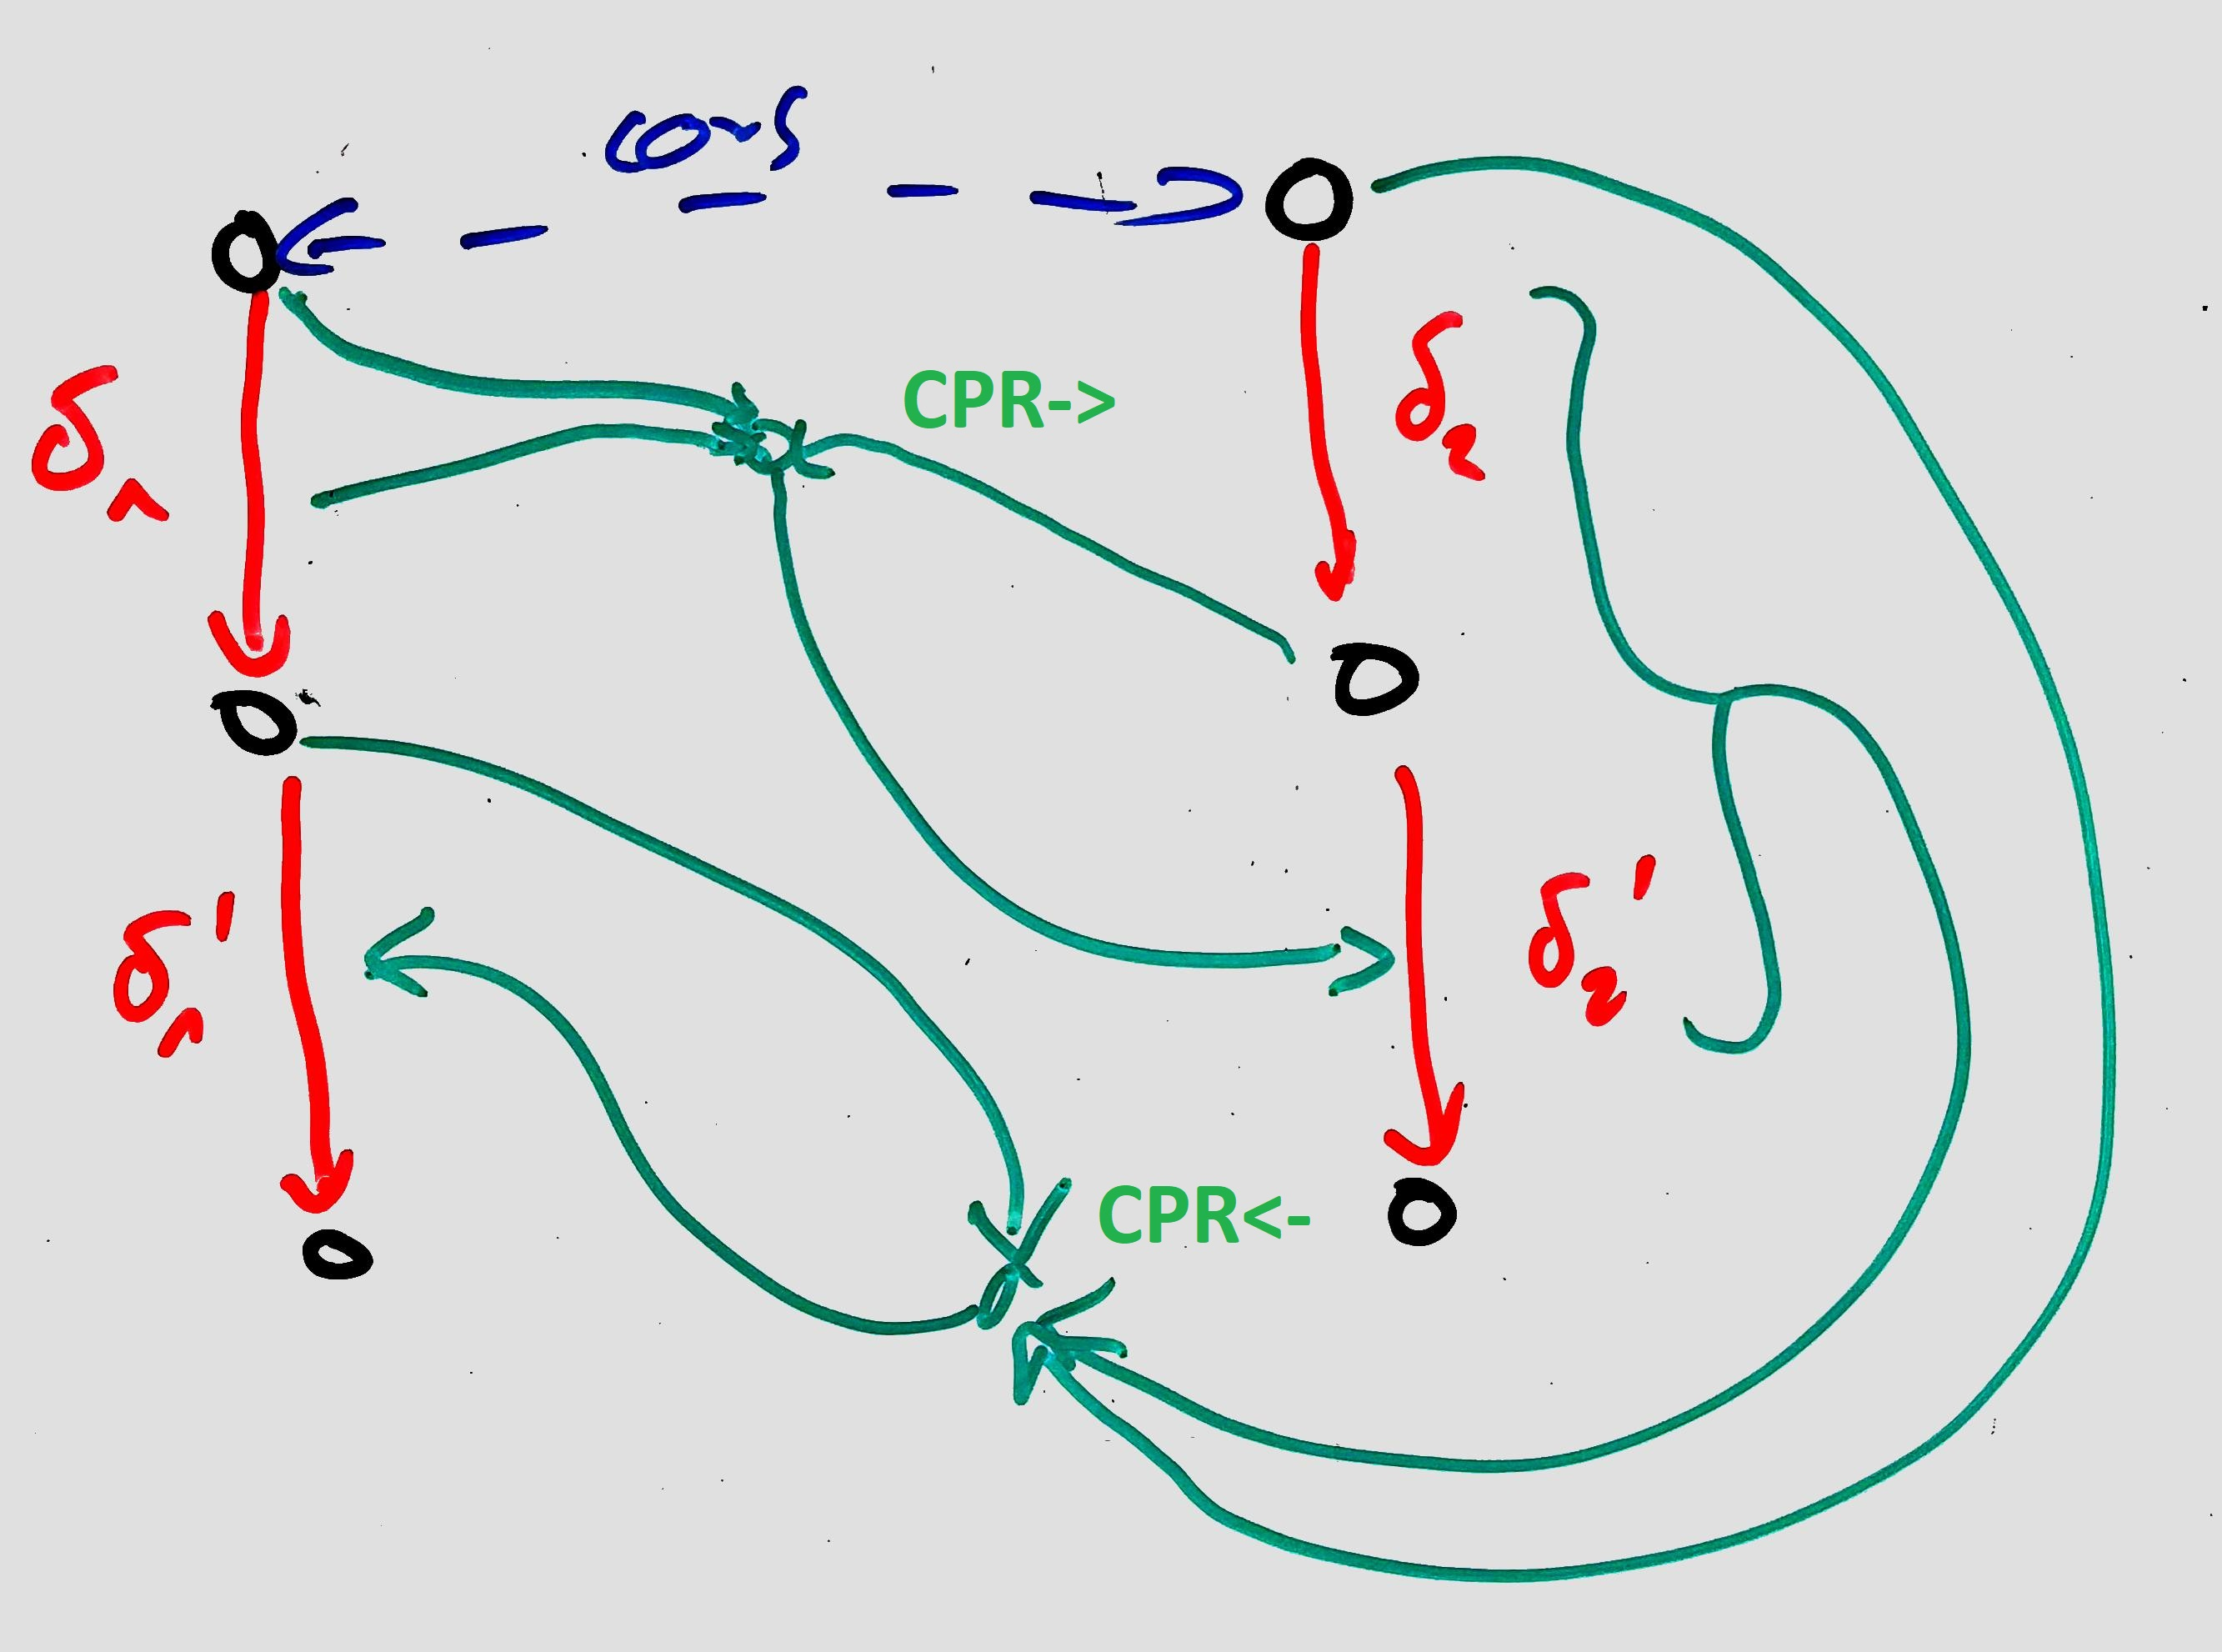
\includegraphics[width=0.7\textwidth]{figures/correctness/synchronization/synchronizing_execution_step.jpg}    
    \caption[Synchronizing bidirectional transformation execution step]{Operation of a synchronizing bidirectional transformation execution step}
    \label{fig:synchronization:synchronizing_execution_step}
\end{figure}

\mnote{Execute step of a transformation to integrate changes to both models}
Since we want consider the case that both of the models instead of only one of them have been modified, we extend the approach to process changes to both models.
More precisely, we introduce a modified notion of transformation execution steps, which is able to process changes to both models.
The operation of that execution step is depicted in \autoref{fig:synchronization:synchronizing_execution_step}.
To this end, the first executed consistency preservation rule is applied to the first model and the change to it, but receives the modified state of the second model.
We have motivated the necessity not to apply the first consistency preservation rule to the unmodified second model in \autoref{chap:synchronization:combination:sequencing}.
Afterwards, we apply the second consistency preservation rule to the unmodified first model and introduce the modifications to the second model as the concatenation of the original change and the one introduced by the first consistency preservation rule.
This way, we ensure that all inconsistencies are introduced by changes that are processed by the consistency preservation rules, which was our requirement for practical applicability due to the necessity only to react to changes instead of processing arbitrarily inconsistent models states.

\begin{definition}[Synchronizing Bidirectional Transformation Execution Step]
    \label{def:synchronizingtransformationexecutionstep}
    Let $\transformation{T} = \tupled{\consistencyrelationset{CR}, \consistencypreservationrule{\consistencyrelationset{CR}}^{\rightarrow}, \consistencypreservationrule{\consistencyrelationset{CR}}^{\leftarrow}}$ be a bidirectional transformation for metamodels $\metamodel{M}{1}$ and $\metamodel{M}{2}$.
    A \emph{synchronizing execution step} $\function{SyncEx}_{\transformation{T}}^1$ of $\transformation{T}$ is a function:
    \begin{align*}
        \function{SyncEx}_{\transformation{T}}^1 : \; & (\metamodelinstanceset{M}{1}, \metamodelinstanceset{M}{2}, \changeuniverse{\metamodel{M}{1}}, \changeuniverse{\metamodel{M}{2}}) \rightarrow (\metamodelinstanceset{M}{1}, \metamodelinstanceset{M}{2}, \changeuniverse{\metamodel{M}{1}}) \cup \setted{\bot} \\
        & (\model{m}{1}, \model{m}{2}, \change{\metamodel{M}{1}}, \change{\metamodel{M}{2}}) \mapsto 
        \begin{cases} 
            (\model{m}{1}', \model{m}{2}', \change{\metamodel{M}{1}}') \\
            \bot
        \end{cases}
    \end{align*}
    with:
    \begin{align*}
        & \change{\metamodel{M}{2}}' = \consistencypreservationrule{\consistencyrelationset{CR}}^{\rightarrow}(\model{m}{1}, \change{\metamodel{M}{2}}(\model{m}{2}), \change{\metamodel{M}{1}}) %\\
        & \model{m}{1}' = \change{\metamodel{M}{1}}(\model{m}{1}) \\
        & \change{\metamodel{M}{1}}' = \consistencypreservationrule{\consistencyrelationset{CR}}^{\leftarrow}(\model{m}{2}, \model{m}{1}', \change{\metamodel{M}{2}}' \concatfunction \change{\metamodel{M}{2}}) %\\
        & \model{m}{2}' = \change{\metamodel{M}{2}}'(\change{\metamodel{M}{2}}(\model{m}{2}))
    \end{align*}
    If either consistency preservation rule is undefined for the input, i.e., $\consistencypreservationrule{\consistencyrelationset{CR}}^{\rightarrow}(\model{m}{1}, \change{\metamodel{M}{2}}(\model{m}{2}), \change{\metamodel{M}{1}}) = \bot$ or $\consistencypreservationrule{\consistencyrelationset{CR}}^{\leftarrow}(\model{m}{2}, \model{m}{1}', \change{\metamodel{M}{2}}' \concatfunction \change{\metamodel{M}{2}}) \bot$, then the execution is undefined, i.e., $\function{SyncEx}_{\transformation{T}}^1(\model{m}{1}, \model{m}{2}, \change{\metamodel{M}{1}}) = \bot$.
    % for given models $\model{m}{1} \in \metamodelinstanceset{M}{1}$, $\model{m}{2} \in \metamodelinstanceset{M}{2}$ and a change $\change{\metamodel{M}{1}} \in \changeuniverse{\metamodel{M}{1}}$ to $\model{m}{1}$ is the consecutive execution of $\consistencypreservationrule{\consistencyrelationset{CR}}^{\rightarrow}$ and $\consistencypreservationrule{\consistencyrelationset{CR}}^{\leftarrow}}$, i.e.
    % \begin{align*}
    %     & \change{\metamodel{M}{2}}' = \consistencypreservationrule{\consistencyrelationset{CR}}^{\rightarrow}(\model{m}{1}, \model{m}{2}, \change{\metamodel{M}{1}}) \\
    %     & \change{\metamodel{M}{1}}' = \consistencypreservationrule{\consistencyrelationset{CR}}^{\leftarrow}(\model{m}{2}, \change{\metamodel{M}{1}}(\model{m}{1}), \change{\metamodel{M}{2}}')
    % \end{align*}
    % with the resulting changes $\change{\metamodel{M}{1}}'$ and $\change{\metamodel{M}{2}}'$.
\end{definition}

\mnote{Synchronization step needs to be executed only once}
The synchronizing bidirectional execution step is necessary to first integrate the changes made in both models.
It is defined such that it only produces a change in the first model, such that afterwards ordinary transformation execution steps that only need to deal with a change to one model have to be applied.
This leads the \autoref{algo:synchronization:executesynchronizingbidirectionaltransformation} for the execution of a synchronizing bidirectional transformation.
%Step integrates both changes, comparable to ordinary step, but first treats changes to m2 as already applied, i.e., given models are inconsistent, then processes the changes in the opposite direction to generate necessary changes to restore consistency from them.

\begin{algorithm}
    \begin{algorithmic}[1]
    \Procedure{\function{ExecuteSync}}{$\transformation{t} = \tupled{\consistencyrelationset{CR}, \consistencypreservationrule{\consistencyrelationset{CR}}^{\rightarrow}, \consistencypreservationrule{\consistencyrelationset{CR}}^{\leftarrow}}, \model{m}{1}, \model{m}{2}, \change{\metamodel{M}{1}}, \change{\metamodel{M}{2}}$}
        \algindentskip
        \If{$\neg (\tupled{\model{m}{1}, \model{m}{2}} \consistenttomath \consistencyrelationset{CR})$}
            \State \Return{$\bot$}
        \EndIf
        \algblockskip

        \If{$\neg (\tupled{\change{\metamodel{M}{1}}(\model{m}{1}), \model{m}{2}} \consistenttomath \consistencyrelationset{CR})$} \label{algo:synchronization:execute_synchronizing_bidirectional_transformation:line:synchronizationstart}
            \State $executionResult$ $\leftarrow$ $\function{SyncEx}_\transformation{t}^1(\model{m}{1}, \model{m}{2}, \change{\metamodel{M}{1}}, \change{\metamodel{M}{2}})$
            \If{$executionResult = \bot$}
                \State \Return{$\bot$} \label{algo:synchronization:execute_synchronizing_bidirectional_transformation:line:returnbot1}
            \Else
                \State $(\model{m}{1}, \model{m}{2}, \change{\metamodel{M}{1}}) \gets executionResult$
            \EndIf
        \EndIf \label{algo:synchronization:execute_synchronizing_bidirectional_transformation:line:synchronizationend}
        \algblockskip

        \While{$\neg (\tupled{\change{\metamodel{M}{1}}(\model{m}{1}), \model{m}{2}} \consistenttomath \consistencyrelationset{CR})$}
            \State $executionResult$ $\leftarrow$ $\function{Ex}_\transformation{t}^1(\model{m}{1}, \model{m}{2}, \change{\metamodel{M}{1}})$
            \If{$executionResult = \bot$}
                \State \Return{$\bot$} \label{algo:execute_synchronizing_bidirectional_transformation:line:returnbot2}
            \Else
                \State $(\model{m}{1}, \model{m}{2}, \change{\metamodel{M}{1}}) \gets executionResult$
            \EndIf
        \EndWhile
        \algblockskip

        \State \Return{$\tupled{\change{\metamodel{M}{1}}(\model{m}{1}), \model{m}{2}}$} \label{algo:synchronization:execute_synchronizing_bidirectional_transformation:line:returnresult}
        \algindentskip
    \EndProcedure
\end{algorithmic}
    \caption[Execution of a bidirectional transformation for synchronization]{Execution of a bidirectional transformation in the synchronization case.}
    \label{algo:synchronization:executesynchronizingbidirectionaltransformation}
\end{algorithm}

\mnote{Synchronizing transformation execution has same properties than non-synchronizing one}
This algorithm has the same properties as the one for the non-synchronization case given in \autoref{algo:synchronization:executebidirectionaltransformation}.
It does always terminate and either returns $\bot$ or a consistent pair of models.

\begin{theorem}[Consistent Termination of Partial-Consistency-Improving Synchronizing Bidirectional Transformation Execution]
    \label{theorem:synchronizingbidirectionaltransformationconsistencytermination}
    Let $\transformation{T} = \tupled{\consistencyrelationset{CR}, \consistencypreservationrule{\consistencyrelationset{CR}}^{\rightarrow}, \consistencypreservationrule{\consistencyrelationset{CR}}^{\leftarrow}}$ be a partial-consistency-improving bidirectional transformation.
    Then \autoref{algo:synchronization:executesynchronizingbidirectionaltransformation} does always terminate and either returns $\bot$ or a consistent model pair.
\end{theorem}
\begin{proof}
    The algorithm is identical to \autoref{algo:synchronization:executebidirectionaltransformation}, except for Lines~\ref{algo:synchronization:executesynchronizingbidirectionaltransformation:line:synchronizationstart}--\ref{algo:synchronization:executesynchronizingbidirectionaltransformation:line:synchronizationend}, which add the initial synchronization step.
    These lines add a single return statement that can return $\bot$.
    Since the return statement not returning $\bot$ is still preceded by the while loop having the loop condition that the model pair needs to be inconsistent, the argument of the proof for \autoref{lemma:bidirectionaltransformationconsistency} regarding non-synchronizing bidirectional transformations ensuring that only consistent models are returned still applies.
    Thus, we know the algorithm either returns $\bot$ or a consistent model pair.

    Termination of the algorithm is guaranteed for the same reasons as for non-synchronizing bidirectional transformations as proven in \autoref{lemma:bidirectionaltransformationtermination}.
    Although the additional execution of $\function{SyncEx}$ may introduce further inconsistencies, the proof already considered that the models given to the while loop may be arbitrarily inconsistent.
    Thus, the inductive improvement in partial consistency through the while loop is given in the same way and thus, finally, the model pair becomes consistent.
\end{proof}

\mnote{Transformation only need to deal with inconsistencies introduced by changes}
Thus, we have proven that we can execute a bidirectional transformation that is partial-consistency-improving for two given models and changes to both of the, such that consistent models are delivered, as long as the transformation is able to process the changes.
In fact, we have already restricted the algorithm such that it must not be able to deal with arbitrarily inconsistent models, but only with models that are initially given, such that only the given changes introduce inconsistencies.
This is supposed to make it easier to define transformation in practice that fulfill the property of being partial-consistency-improving, as they can rely on the assumption that inconsistency is only introduced by the given changes.

\mnote{Definition of synchronizing bidirectional transformations}
With the insight that partial-consistency-improving bidirectional transformations can be used to integrate changes to both of two models and deliver consistent models based on that changes, we can define \emph{synchronizing bidirectional transformations} as bidirectional transformations with the property of being partial-consistency-improving.

\begin{definition}[Synchronizing Bidirectional Transformation]
    Let $\transformation{T}$ be a partial-consistency-improving bidirectional transformation.
    Then we call $\transformation{T}$ a \emph{synchronizing bidirectional transformation}.
\end{definition}

\mnote{Order of consistency preservation rules provides no conceptual benefit but may improve usability}
As we have already discussed at the end of \autoref{chap:synchronization:bidirectional:transformations}, we defined bidirectional transformation execution steps starting with $\consistencypreservationrule{\consistencyrelationset{CR}}^{\rightarrow}$, although it may also be necessary to start with $\consistencypreservationrule{\consistencyrelationset{CR}}^{\leftarrow}$ if a change was performed in the second model.
We discussed that our definitions are without loss of generality and can be directly transferred by swapping the rules.
For the synchronization case, in which both models have been modified, it does, theoretically, not even make a difference which of the consistency preservation rules is executed first, because changes to both models are present anyway.
From a practical perspective, it can, however, make sense to define one the consistency preservation rules as the one to always be executed first.
For example, it might make sense to first execute the consistency preservation rule from the more abstract to the more detailed model, if such a relation exists between the models.
We leave such considerations up to the individual transformation developer or future research, as the selection of the order does not provide any conceptual benefits, but, in the best case, eases the definition of appropriate consistency preservation rules and improves usability.

\todo{Define synchronizing bidirectional transformation as a partial-consistency-improving bidirectional transformation}


\subsection{Equivalence to Synchronizing Transformations}

\mnote{Synchronizing and synchronizing bidirectional transformations have equal inputs and outputs}
For our definition of transformation networks, we used the notion of synchronizing transformations (cf.~\autoref{def:synchronizingtransformation}), whose single consistency preservation rule accept two consistent models and a change to each of them and return two changes that, if applied to the models, result in consistent models again.
Synchronizing bidirectional transformations, i.e., the yet defined transformations, which are composed of two unidirectional consistency preservation rules, also accept two consistent models and a change to each of them and return two consistent models.
We could also define those transformations to return changes rather than the consistent models by simply concatenating all changes calculated by the transformation execution steps.
For reasons of simplicity, we omitted that in the formal description.

\mnote{Synchronizing and synchronizing bidirectional transformations have equal expressiveness}
Although synchronizing transformations and synchronizing bidirectional transformations have the same requirements to their inputs and provide the same guarantees regarding consistency for their output, both may also return $\bot$ to indicate that they were not able to calculate changes that lead to consistent models.
While a synchronizing transformation can be defined such that it never return $\bot$ by defining a consistency preservation rule that is a total function, the possibility of a synchronizing bidirectional transformation to never return $\bot$ depends on the interplay of the two unidirectional consistency preservation rules.
Nevertheless, we can show that both have equal expressiveness, i.e., they can always return the same results for the same inputs.

\begin{theorem}[Synchronizing Bidirectional Transformation Expressiveness]
    Synchronizing bidirectional transformations have equal expressiveness than synchronizing transformations.
\end{theorem}
\begin{proof}
    Each synchronizing bidirectional transformation can be realized by a synchronizing transformation by simply defining the function of the consistency preservation rule such that it returns the result that is produced by the execution of the synchronizing bidirectional transformation.
    Let $\transformation{T}$ be a synchronizing bidirectional transformation with:
    \begin{align*}
        \function{ExecuteSync}(\transformation{T}, \model{m}{1}, \model{m}{2}, \change{\metamodel{M}{2}}) = (\model{m}{1}', \model{m}{2}')
    \end{align*}
    Then we define the consistency preservation rule $\consistencypreservationrule{}$ of a synchronizing transformation as:
    \begin{align*}
        &
        \consistencypreservationrule{}(\model{m}{1}, \model{m}{2}, \change{\metamodel{M}{1}}, \change{\metamodel{M}{2}}) = (\model{m}{1}, \model{m}{2}, \change{\metamodel{M}{1}}', \change{\metamodel{M}{2}}') \\
        & \formulaskip
        \mathtext{with} \change{\metamodel{M}{1}}'(\change{\metamodel{M}{1}}(\model{m}{1})) \equivalentperdefinition \model{m}{1}' 
        \land \change{\metamodel{M}{2}}'(\change{\metamodel{M}{2}}(\model{m}{2})) \equivalentperdefinition \model{m}{2}'
    \end{align*}
    Then, per definition, applying the resulting changes to the input models, the synchronizing transformation delivers for every possible input the same result by applying $\consistencypreservationrule{}$ as the synchronizing bidirectional transformation.

    Realizing a synchronizing transformation by a synchronizing bidirectional transformation requires the repeated execution of the two consistency preservation rules to emulate the behavior of the single 
    synchronizing consistency preservation rule.
    Let $\consistencypreservationrule{}$ be the consistency preservation rule of a synchronizing transformation with:
    \begin{align*}
        \consistencypreservationrule{}(\model{m}{1},\model{m}{2},\change{\metamodel{M}{1}},\change{\metamodel{M}{2}}) = (\model{m}{1},\model{m}{2},\change{\metamodel{M}{1}}',\change{\metamodel{M}{2}}')
    \end{align*}
    Then we can define the two unidirectional consistency preservation rules of the synchronizing transformation $\transformation{T}$ as follows.
    \begin{align*}
        & 
        \consistencypreservationrule{}^{\rightarrow}(\model{m}{1},\change{\metamodel{M}{2}}(\model{m}{2}),\change{\metamodel{M}{1}}) = \change{\metamodel{M}{2}}'' \mathtext{with} \change{\metamodel{M}{2}}''(\change{\metamodel{M}{2}}(\model{m}{2})) \equivalentperdefinition \change{\metamodel{M}{2}}'(\model{m}{2}) \\
        &
        \consistencypreservationrule{}^{\leftarrow}(\model{m}{2},\change{\metamodel{M}{1}}(\model{m}{1}),\change{\metamodel{M}{2}}'' \concatfunction \change{\metamodel{M}{2}}) = \change{\metamodel{M}{1}}'' \mathtext{with} \change{\metamodel{M}{1}}''(\change{\metamodel{M}{1}}(\model{m}{1})) \equivalentperdefinition \change{\metamodel{M}{1}}'(\model{m}{1})
    \end{align*}
    So we simply define the two consistency preservation rules in a way such that each of them delivers for the inputs in the synchronizing execution step $\function{SyncEx}_{\transformation{T}}^1$ according to \autoref{def:synchronizingtransformationexecutionstep} those changes that are necessary to produce exactly the results of the consistency preservation rule $\consistencypreservationrule{}$ of the synchronizing transformation.
    Then according to the behavior of $\function{SyncEx}_{\transformation{T}}^1$, we have:
    \todo{Vielleicht besser Striche über Buchstaben statt noch mehr Apostrophe}
    \begin{align*}
        &
        \function{SyncEx}_{\transformation{T}}^1(\model{m}{1},\model{m}{2},\change{\metamodel{M}{1}},\change{\metamodel{M}{2}}) = (\model{m}{1}'', \model{m}{2}'', \change{\metamodel{M}{1}}''') \mathtext{with} \\
        & \formulaskip
        \change{\metamodel{M}{1}}'''(\model{m}{1}'') = % per def SyncEx
        \change{\metamodel{M}{1}}'''(\change{\metamodel{M}{1}}(\model{m}{1})) = % per def SyncEx and per def above
        %\consistencypreservationrule{}^{\leftarrow}(\model{m}{2},\change{\metamodel{M}{1}}(\model{m}{1}),\change{\metamodel{M}{2}}'' \concatfunction \change{\metamodel{M}{2}})(\change{\metamodel{M}{1}}(\model{m}{1})) % per def above
        \change{\metamodel{M}{1}}'(\model{m}{1}) \\
        & \formulaskip
        \land
        \model{m}{2}'' = \change{\metamodel{M}{2}}'(\model{m}{2})
    \end{align*}
    So $\function{SyncEx}_{\transformation{T}}^1$ produces $\model{m}{1}''$, $\model{m}{2}''$ and $\change{\metamodel{M}{1}}'''$ for which we know that $\change{\metamodel{M}{1}}'''(\model{m}{1}'')$ and $\model{m}{2}''$ are consistent, because their equivalents $\change{\metamodel{M}{1}}'(\model{m}{1})$ and $\change{\metamodel{M}{2}}'(\model{m}{2})$ are consistent by assumption.
    Thus, the execution of the synchronizing bidirectional transformation $\transformation{T}$ according to \autoref{algo:synchronization:executesynchronizingbidirectionaltransformation} terminates after the conditional statement in \autoref{algo:synchronization:executesynchronizingbidirectionaltransformation:line:synchronizationstart} with the same consistent models that are delivered by the applying the changes calculated by the consistency preservation rule $\consistencypreservationrule{}$ of the assumed synchronizing transformation.

    With these construction approaches in both directions, we have shown that each synchronizing transformation can be expressed by a synchronizing bidirectional transformation and vice versa.
\end{proof}

\mnote{Executing only one synchronizing execution step will not lead to consistency in pratice}
Although we have proven that each synchronizing transformation can be expressed by a synchronizing bidirectional transformations and thus the latter ones can be used to express any desired consistency preservation in a transformation network, the constructive approach in the proof does not reflect a practical construction approach for the unidirectional consistency preservation rules of a synchronizing bidirectional transformation.
In practice, it will usually not be possible to define the rules in a way that they deliver consistent models after executing each ones, as we already discussed in \autoref{chap:synchronization:combination:bounds}.
It shows, however, that it would possible in theory.

\mnote{Synchronizing bidirectional transformations can be used in transformation networks}
Based on the knowledge that we can use synchronizing bidirectional transformations in transformation networks, we discuss in the following how a transformation developer can actually achieve that the specification of a bidirectional transformation in terms of two unidirectional consistency preservation rules does actually fulfill the requirements of being partial-consistency-improving and thus synchronizing.


% We yet discussed how to integrate one change on partially consistent models.
% Now we apply to this be able to integrate changes to both models.
% Describe the process here:

% Two step process.
% 1 Integrate changes to both models.
% d2' = CPRr(m1, d2(m2), d1) und d1' = CPRl(m2, d1(m1), d2' o d2)
% 2. Iteratively propagate changes.
% d2'' = CPRr(d1(m1), d2' o d2(m2), d1')
% d1'' = CPRl(d2' o d2(m2), d1(m1), d2'')
% etc. 

% The first step is special, because CPRl needs to process both the original changes as well as the ones generated by CPRr in the first step.
% In all further steps it is only necessary to process the changes just generated by the other CPR.

% DISCUSS: Which CPR to execute first? One is the "leading" one. Integrate its changes first. Can be determined by abstraction, or, theoretically, it completely irrelevant. Only a practical consideration.



% \section{Old contents to integrate}

%%
%% THE DIRECTIONALITY GAP: Formal framework considers bidirectional transformations, practically we have unidirectional ones
%%
% \subsection{The Directionality Gap}

% \mnote{Unidirectional synchronizing preservation rules to close the gap}
% To come up with an approach to combine unidirectional consistency preservation rules to behave as a single synchronizing one, we first identify how we can decompose synchronizing consistency preservation rules into unidirectional ones.
% We then relate these unidirectional synchronizing rules to the non-synchronizing ones defined in transformation languages.

% \mnote{Fine-grained consistency relations allow to define relation between unidirectional preservation rules}
% In \autoref{chap:compatibility:formal_notion}, we also discussed that consistency relation can be considered in a fine-grained way that is able to reflect different notion of consistency in both directions of a relation.
% We will base our notion of unidirectional synchronizing rules on those fine-grained relations to be able to find a proper notion of how the rules in both directions are supposed to work together.
% We did, however, also discuss in that chapter that all fine-grained relations can also be translated into \modellevelconsistencyrelations, thus the insights we already had for those model-level relations still apply to the considerations regarding fine-grained ones.

% \mnote{Stick to coarse-grained notion of preservation rules}
% According to the consideration of fine-grained consistency relations, transformation languages also allow the specification of or derive fine-grained consistency preservation rules from a declarative specification.
% They are often called \emph{transformation rules} and composed to a transformation that consists of multiple such rules, each encoding a consistency relations and a preservation rule for it.
% We will, however, stick to the coarse-grained notion of consistency preservation rules, as they are sufficient for our considerations.

% \mnote{New transformation notion based on fine-grained consistency relations}
% In consequence, from now we will consider a synchronizing transformation as a set of fine-grained consistency relations according to \autoref{def:consistencyrelation} and a consistency preservation rule that preserves consistency according to the set of relations.
% The consistency preservation rule and also the complete transformation are thus still considered correct if applying it to a consistent pair of models and changes to them, applying the resulting changes to the models again delivers a pair of models that is consistent to all consistency relations.
% Note that being consistent to all fine-grained consistency relations is equivalent to being consistent to the single \modellevelconsistencyrelation induced by the fine-grained relations.


% \subsubsection{Unidirectional Synchronizing Transformations}

% \mnote{Decomposition of consistency preservation rules into two unidirectional ones}
% To reflect the unidirectional notion of consistency preservation provided by transformation languages in our formalism, we propose a decomposition of consistency preservation rules according to \autoref{def:consistencypreservationrule} into two unidirectional ones.

% \begin{definition}[Unidirectional Consistency Preservation Rule]
%     \label{def:unidirectionalconsistencypreservationrule}
%     Let $\metamodel{M}{1}, \metamodel{M}{2}$ be two metamodels and $\consistencyrelationset{CR}$ a set of consistency relations between elements of those metamodels.
%     A \emph{unidirectional consistency preservation rule} $\consistencypreservationrule{\consistencyrelationset{CR}}$ for the relation set $\consistencyrelationset{CR}$ is a function:
%     \begin{align*}
%         \consistencypreservationrule{\consistencyrelationset{CR}} : (\metamodelinstanceset{M}{1}, \metamodelinstanceset{M}{2}, \changeuniverse{\metamodel{M}{1}}, \changeuniverse{\metamodel{M}{2}}) \rightarrow \changeuniverse{\metamodel{M}{2}}
%     \end{align*}
% \end{definition}

% \mnote{Notation for two related unidirectional rules}
% To be able to explicitly reference the consistency preservation rules for both directions between two metamodels $\metamodel{M}{1}$ and $\metamodel{M}{2}$, we denote the set of consistency relations between $\metamodel{M}{1}$ and $\metamodel{M}{2}$ as $\consistencyrelationset{CR}_{\rightarrow}$ and the one in the opposite direction between $\metamodel{M}{2}$ and $\metamodel{M}{1}$ as $\consistencyrelationset{CR}_{\leftarrow}$.
% We then refer to the two unidirectional consistency preservation rules as:
% \begin{align*}
%     \consistencypreservationrule{\consistencyrelationset{CR}_{\rightarrow}} : (\metamodelinstanceset{M}{1}, \metamodelinstanceset{M}{2}, \changeuniverse{\metamodel{M}{1}}) \rightarrow \changeuniverse{\metamodel{M}{2}}\\
%     \consistencypreservationrule{\consistencyrelationset{CR}_{\leftarrow}} : (\metamodelinstanceset{M}{2}, \metamodelinstanceset{M}{1}, \changeuniverse{\metamodel{M}{2}}) \rightarrow \changeuniverse{\metamodel{M}{1}}
% \end{align*}

% \mnote{Correctness of unidirectional rules analogous to original rules}
% We define correctness of such a unidirectional consistency preservation rule in the same way it was defined for synchronizing consistency preservation rules according to \autoref{def:consistencypreservationrule} and compliant to existing correctness notions for non-synchronizing consistency preservation rules, such as~\cite{stevens2010sosym}.

% \begin{definition}[Unidirectional Consistency Preservation Rule Correctness]
%     \label{def:unidirectionalconsistencypreservationrulecorrectness}
%     Let $\consistencypreservationrule{\consistencyrelationset{CR}}$ be a \emph{unidirectional consistency preservation rule}.
%     We call $\consistencypreservationrule{\consistencyrelationset{CR}}$ \emph{correct} if the resulting models when applying the generated changes are consistent to $\consistencyrelationset{CR}$ again:
%     \begin{align*}
%         &
%         \forall 
%         \model{m}{1} \in \metamodelinstanceset{M}{1}, 
%         \model{m}{2} \in \metamodelinstanceset{M}{2},
%         \change{\metamodel{M}{1}} \in \changeuniverse{\metamodel{M}{1}},
%         \change{\metamodel{M}{2}} \in \changeuniverse{\metamodel{M}{2}} : \\
%         & \formulaskip
%         \tupled{\model{m}{1}, \model{m}{2}} \consistenttomath \consistencyrelationset{CR} \\
%         & \formulaskip
%         \land \exists 
%         \change{\metamodel{M}{2}}' \in \changeuniverse{\metamodel{M}{2}} :
%         \change{\metamodel{M}{2}}' = \consistencypreservationrule{\consistencyrelation{CR}{}}(\model{m}{1}, \model{m}{2}, \change{\metamodel{M}{1}}, \change{\metamodel{M}{2}}) \\
%         & \formulaskip\formulaskip
%         \Rightarrow
%         \tupled{\change{\metamodel{M}{1}}(\model{m}{1}), \change{\metamodel{M}{2}}'(\model{m}{2})} \consistenttomath \consistencyrelationset{CR}
%     \end{align*}
% \end{definition}

% \mnote{Unidirectional synchronizing transformation encapsule a preservation rule for each direction}
% Based on such a unidirectional notion of consistency preservation rule, we can also define a unidirectional notion of transformations, which then consists of two sets of unidirectional consistency relations and two unidirectional consistency preservation rules.

% \begin{definition}[Unidirectional Synchronizing Transformation]
%     \label{def:unidirectionalsynchronizingtransformation}
%     Let $\metamodel{M}{1}$ and $\metamodel{M}{2}$ be two metamodels and $\consistencyrelationset{CR}_{\rightarrow}$ a set of consistency relations between $\metamodel{M}{1}$ and $\metamodel{M}{2}$, as well as $\consistencyrelationset{CR}_{\leftarrow}$ a set of consistency relations between $\metamodel{M}{2}$ and $\metamodel{M}{1}$.
%     Additionally, let $\consistencypreservationrule{\consistencyrelationset{CR}_{\rightarrow}}$ and $\consistencypreservationrule{\consistencyrelationset{CR}_{\leftarrow}}$ be unidirectional consistency preservation rules for both consistency relation sets.
%     A \emph{unidirectional synchronizing transformation} is a quadruple $\transformation{T} = \tupled{\consistencyrelationset{CR}_{\rightarrow}, \consistencyrelationset{CR}_{\leftarrow},\consistencypreservationrule{\consistencyrelationset{CR}_{\rightarrow}}, \consistencypreservationrule{\consistencyrelationset{CR}_{\leftarrow}}}$.
% \end{definition}

% \mnote{Correctness of unidirectional synchronizing transformations}
% We call such a unidirectional synchronizing transformation correct if both consistency preservation rules are correct, i.e., they both preserve consistency according to the underlying consistency relation set.

% \begin{definition}[Unidirectional Synchronizing Transformation Correctness]
%     \label{def:unidirectionalsynchronizingtransformationcorrectness}
%     Let $\transformation{T} = \tupled{\consistencyrelationset{CR}_{\rightarrow}, \consistencyrelationset{CR}_{\leftarrow},\consistencypreservationrule{\consistencyrelationset{CR}_{\rightarrow}}, \consistencypreservationrule{\consistencyrelationset{CR}_{\leftarrow}}}$ be a unidirectional synchronizing transformation.
%     We call $\transformation{T}$ correct if, and only if, $\consistencypreservationrule{\consistencyrelationset{CR}_{\rightarrow}}$ and $\consistencypreservationrule{\consistencyrelationset{CR}_{\leftarrow}}$ are both correct according to \autoref{def:unidirectionalconsistencypreservationrulecorrectness}.
% \end{definition}

% \mnote{Each unidirectional rule only preserves consistency in one direction}
% With a unidirectional synchronizing transformation that adheres to the given correctness definition, we are able to preserve consistency for the consistency relations in each direction between two models.
% Executing either of the unidirectional consistency preservation rules of the transformation does, however, not ensure that the consistency relations for the other direction are fulfilled as well.
% That is the purpose of the other unidirectional consistency preservation rule.

% % \begin{itemize}
%     % \item We assume consistency preservation rules according to fine-grained consistency relations introduced for compatibility
%     % \item So a synchronizing transformation considers fine-grained relations, in fact a transformation then consists of multiple relations, two for each fine-grained relation (each direction). Their combination induces the \modellevelconsistencyrelation for the two metamodels.
%     % \item Although the consistency preservation rule may in practice also be defined in terms fine-grained rules, which together with the fine-grained consistency rules then forms what is often called \emph{transformation rules}, we do not need to have a more fine-grained notion here.
%     % \item The transformation then is still correct as defined before, when the preservation rule preserves consistency to the relation, but now according to all fine-grained relations (and thus also the induced monolithic one) instead to the single model-level one.
%     % \item To reflect the notion of unidirectional consistency preservation rules, as often defined in transformation languages, which are still synchronizing, i.e., are able to react to changes made to both models, we may define:
% % \end{itemize}
% % \begin{align*}
% %     \consistencypreservationrule{\consistencyrelationset{CR}_{\rightarrow},\rightarrow} : (\metamodelinstanceset{M}{1}, \metamodelinstanceset{M}{2}, \changeuniverse{\metamodel{M}{1}}, \changeuniverse{\metamodel{M}{2}}) \rightarrow \changeuniverse{\metamodel{M}{2}})\\
% %     \consistencypreservationrule{\consistencyrelationset{CR}_{\leftarrow},\leftarrow} : (\metamodelinstanceset{M}{1}, \metamodelinstanceset{M}{2}, \changeuniverse{\metamodel{M}{1}}, \changeuniverse{\metamodel{M}{2}}) \rightarrow \changeuniverse{\metamodel{M}{1}})
% % \end{align*}

% \subsubsection{Alignment of Unidirectional Synchronizing Transformations}

% \mnote{Sequential execution of unidirectional rules does not guarantee consistency to relations in both directions}
% It is now possible to execute both consistency preservation rules of a unidirectional synchronizing transformation one after another, as each is able to reflect the changes produced by the other due to the ability to process changes made to both models.
% Thus, we could sequentially calculate:
% \begin{align*}
%     &
%     \change{\metamodel{M}{2}}' = \consistencypreservationrule{\consistencyrelationset{CR}_{\rightarrow}}(\model{m}{1},\model{m}{2},\change{\metamodel{M}{1}},\change{\metamodel{M}{2}})\\
%     &
%     \change{\metamodel{M}{1}}' = \consistencypreservationrule{\consistencyrelationset{CR}_{\leftarrow}}(\model{m}{2},\model{m}{1},\change{\metamodel{M}{2}}',\change{\metamodel{M}{1}})
% \end{align*}
% We then receive the resulting model pair as $\tupled{\change{\metamodel{M}{1}}'(\model{m}{1}), \change{\metamodel{M}{2}}'(\model{m}{2})}$.
% This gives us the guarantee that the resulting model pair is consistent to $\consistencyrelationset{CR}_{\leftarrow}$, as its consistency preservation rule was executed last.
% However, the definitions do not give any guarantee that the model pair is consistent to $\consistencyrelationset{CR}_{\rightarrow}$, as the execution of $\consistencypreservationrule{\consistencyrelationset{CR}_{\leftarrow}}$ may violate some of those relations.

% \mnote{Not violating relations of the other direction is desirable for unidirectional rules}
% It is, however, a desirable property of a unidirectional synchronizing transformation that the consistency preservation rules for the two directions between the same metamodels are aligned with each other in a way that executing the rule in one direction does not lead to further violations of the consistency relations in the other direction.
% This is especially necessary to produce the same behavior as a synchronizing transformation.
% We call such a property \emph{inverse-preserving}, as it ensures that fulfillment of consistency relations of the inverse direction are preserved.

% \begin{definition}[Inverse-Preserving Unidirectional Synchronizing Transformation]%Unidirectional Consistency Preservation Rule}
%     \label{def:inversepreservingunidirectionalsynchronizingtransformation}
%     Let $\transformation{T} = \tupled{\consistencyrelationset{CR}_{\rightarrow}, \consistencyrelationset{CR}_{\leftarrow},\consistencypreservationrule{\consistencyrelationset{CR}_{\rightarrow}}, \consistencypreservationrule{\consistencyrelationset{CR}_{\leftarrow}}}$ be a correct unidirectional synchronizing transformation for two metamodels $\metamodel{M}{1}$ and $\metamodel{M}{2}$.
%     We say that $\transformation{T}$ is \emph{inverse-preserving} if, and only if, executing one of the consistency preservation rules ensures that the resulting models are still consistent to all consistency relations of the opposite direction to which the models were consistent before.
%     For $\consistencypreservationrule{\consistencyrelationset{CR}_{\rightarrow}}$ this is given by the following (for $\consistencypreservationrule{\consistencyrelationset{CR}_{\leftarrow}}$ analogously):
%     \begin{align*}
%         & \forall \model{m}{1} \in \metamodelinstanceset{M}{1}, \model{m}{2} \in \metamodelinstanceset{M}{2}, \change{\metamodel{M}{1}} \in \changeuniverse{\metamodel{M}{1}}, \change{\metamodel{M}{2}} \in \changeuniverse{\metamodel{M}{2}} : \\
%         & 
%         \exists \change{\metamodel{M}{2}}' \in \changeuniverse{\metamodel{M}{2}} : \change{\metamodel{M}{2}}' = \consistencypreservationrule{\consistencyrelationset{CR}_{\rightarrow}}(\model{m}{1},\model{m}{2},\change{\metamodel{M}{1}},\change{\metamodel{M}{2}}) \\
%         & \formulaskip
%         \Rightarrow
%         \forall \consistencyrelation{CR}{} \in \consistencyrelationset{CR}_{\leftarrow}: 
%         \bigl(
%         \tupled{\change{\metamodel{M}{2}}(\model{m}{2}),\change{\metamodel{M}{1}}(\model{m}{1})} \consistenttomath \consistencyrelation{CR}{} \\
%         & \formulaskip\formulaskip
%         \Rightarrow
%         \tupled{\change{\metamodel{M}{2}}'(\model{m}{2}), \change{\metamodel{M}{1}}(\model{m}{1})} \consistenttomath \consistencyrelation{CR}{}
%         \bigr)
%     \end{align*}
% \end{definition}

% \mnote{Inverse-preserving transformations define reasonable alignment}
% This is a reasonable property, because the consistency relations in both directions are usually not disaligned, but only give the freedom to define different consistency notions in both directions, such as more options for consistent elements in one direction than in the other to support different kinds of abstraction.
% It should, however, never be the case that preserving consistency in one direction violates consistency relations in the other direction if transformations are defined properly.

% \mnote{Inverse-preserving transformations can be sequences}
% Given an inverse-preserving unidirectional synchronizing transformation, executing the two unidirectional consistency preservation rules one after another to given consistent models and changes to them preserves consistency to all consistency relations.
% This is a direct consequence of the inverse-preserving property, because no directional rule is allowed to violate consistency that was already ensured in the other direction.

% \begin{theorem}[Inverse-Preserving Unidirectional Synchronizing Transformation Sequencing Correctness]
%     \label{theorem:sequencinginversepreservingtransformations}
%     Let $\transformation{T} = \tupled{\consistencyrelationset{CR}_{\rightarrow}, \consistencyrelationset{CR}_{\leftarrow}, \consistencypreservationrule{\consistencyrelationset{CR}_{\rightarrow}}, \consistencypreservationrule{\consistencyrelationset{CR}_{\leftarrow}}}$ be a correct, inverse-preserving unidirectional synchronizing transformation.
%     Then sequentially executing both consistency preservation rules to given models and changes restores consistency to both consistency relation sets, i.e., given models $\model{m}{1}, \model{m}{2}$ and changes to them $\change{\metamodel{M}{1}}, \change{\metamodel{M}{2}}$, it holds hat:
%     \begin{align*}
%         &
%         \tupled{\model{m}{1}, \model{m}{2}} \consistenttomath \consistencyrelationset{CR}_{\rightarrow}
%         \land \tupled{\model{m}{2}, \model{m}{1}} \consistenttomath \consistencyrelationset{CR}_{\leftarrow}\\
%         &
%         \land \exists \change{\metamodel{M}{2}}' \in \changeuniverse{\metamodel{M}{2}}' : 
%         \change{\metamodel{M}{2}}' = \consistencypreservationrule{\consistencyrelationset{CR}_{\rightarrow}}(\model{m}{1}, \model{m}{2}, \change{\metamodel{M}{1}}, \change{\metamodel{M}{2}}) \\
%         &
%         \land \exists \change{\metamodel{M}{1}}' \in \changeuniverse{\metamodel{M}{1}}' :
%         \change{\metamodel{M}{1}}' = \consistencypreservationrule{\consistencyrelationset{CR}_{\leftarrow}}(\model{m}{2}, \model{m}{1}, \change{\metamodel{M}{2}}', \change{\metamodel{M}{1}}) \\
%         &
%         \Rightarrow \tupled{\change{\metamodel{M}{1}}'(\model{m}{1}), \change{\metamodel{M}{2}}'(\model{m}{2})}\consistenttomath \consistencyrelationset{CR}_{\rightarrow}  \\
%         & \formulaskip
%         \land \tupled{\change{\metamodel{M}{2}}'(\model{m}{2}), \change{\metamodel{M}{1}}'(\model{m}{1})} \consistenttomath \consistencyrelationset{CR}_{\leftarrow}
%     \end{align*}
% \end{theorem}
% \begin{proof}
%     Given models $\model{m}{1}, \model{m}{2}$ that are consistent to $\consistencyrelationset{CR}_{\rightarrow}$ and $\consistencyrelationset{CR}_{\leftarrow}$ and changes $\change{\metamodel{M}{1}}, \change{\metamodel{M}{2}}$, we assume that $\change{\metamodel{M}{1}}'$ and $\change{\metamodel{M}{2}}'$ exist as the results of the consistency preservation rules according to the theorem.
%     If this was not the case, the consistency preservation rules are not defined for the given inputs and thus are not able to produce consistent results, which evaluates the left side of the implication to false, making the whole statement of the theorem true.
%     Now we show correctness of both implied statements:
%     \begin{properenumerate}
%         \item $\tupled{\change{\metamodel{M}{1}}'(\model{m}{1}), \change{\metamodel{M}{2}}'(\model{m}{2})}\consistenttomath \consistencyrelationset{CR}_{\rightarrow}$:
%         As a direction implication of correctness of $\consistencypreservationrule{\consistencyrelationset{CR}_{\rightarrow}}$, we know that $\tupled{\change{\metamodel{M}{1}}(\model{m}{1}), \change{\metamodel{M}{2}}'(\model{m}{2})} \consistenttomath \consistencyrelationset{CR}_{\rightarrow}$.
%         Now the inverse-preserving property of $\transformation{T}$ ensures for the given input of $\consistencypreservationrule{\consistencyrelationset{CR}_{\leftarrow}}$ according to \autoref{def:inversepreservingunidirectionalsynchronizingtransformation} that 
%         \begin{align*}
%         & \forall \consistencyrelation{CR}{} \in \consistencyrelationset{CR}_{\rightarrow}: 
%         \bigl(
%         \tupled{\change{\metamodel{M}{1}}(\model{m}{1}),\change{\metamodel{M}{2}}'(\model{m}{2})} \consistenttomath \consistencyrelation{CR}{} \\
%         & \formulaskip\formulaskip
%         \Rightarrow
%         \tupled{\change{\metamodel{M}{1}}'(\model{m}{2}), \change{\metamodel{M}{2}}'(\model{m}{1})} \consistenttomath \consistencyrelation{CR}{}
%         \bigr)
%         \end{align*}
%         Since the left side of the implication is true for all consistency relations in $\consistencyrelationset{CR}_{\rightarrow}$ due to correctness of $\consistencypreservationrule{\consistencyrelationset{CR}_{\rightarrow}}$, the right side is also true for all consistency relations in $\consistencyrelationset{CR}_{\rightarrow}$.
%         In consequence, we know that $\tupled{\change{\metamodel{M}{1}}'(\model{m}{1}), \change{\metamodel{M}{2}}'(\model{m}{2})} \consistenttomath \consistencyrelationset{CR}_{\rightarrow}$
%         \item $\tupled{\change{\metamodel{M}{2}}'(\model{m}{2}), \change{\metamodel{M}{1}}'(\model{m}{1})} \consistenttomath \consistencyrelationset{CR}_{\leftarrow}$:
%         This directly follows from correctness of $\consistencypreservationrule{\consistencyrelationset{CR}_{\leftarrow}}$.
%     \end{properenumerate}
%     In consequence, sequentially applying both consistency preservation rules of an inverse-preserving unidirectional synchronizing transformation ensures consistency to the consistency relations in both directions.
% \end{proof}

% \mnote{Inverse-preserving unidirectional transformation can emulate synchronizing ones}
% As a consequence of the theorem, we know that we can emulate a synchronizing transformation according to \autoref{def:synchronizingtransformation} with an inverse-preserving unidirectional synchronizing transformation according to \autoref{def:inversepreservingunidirectionalsynchronizingtransformation}.
% We can execute the unidirectional consistency preservation rules one after another to achieve that the resulting models are consistent to all consistency relations in both direction.

% \mnote{Ensuring inverse-preserving property is already a problem of bidirectional transformations}
% In fact, it is not trivial to ensure that two unidirectional transformations are inverse-preserving, even if the consistency relations in both directions are the same, which we will also see in our evaluation of errors in \autoref{chap:errors}.
% This problem, however, already arises when defining bidirectional transformations.
% Transformation languages may derive two unidirectional preservation rules from one specification, so that they are inherently inverse-preserving, or they may allow individual specification of the directions and provide some support for checking that they are aligned with each other, e.g., in the sense that they are inverse-preserving.
% This is, however, an isolated and existing topic of research \todo{Add references for that} and a challenge that already has to be solved for a single bidirectional transformation rather than a network, which is why we do not discuss this problem in more detail here and therefore assume given transformations to be inverse-preserving.

% \mnote{Directionality gap was discussed, synchronization gap remains}
% We have discussed the gap between synchronizing transformations and ordinary transformations defined in transformation languages regarding directionality by decomposing synchronizing transformations into unidirectional ones.
% In the following, we discuss the remaining gap of the formalized transformations being synchronizing, whereas practically defined transformations do not have that property.


%%
%% THE SYNCHRONIZATION GAP: After the directionality gap, we need to discuss how to come from synchronizing to non-synchronizing transformations
%%
% \subsection{The Synchronization Gap}

% \mnote{Practical transformations are not synchronizing}
% Still, there is a gap to practical approaches for defining transformations, as existing approaches do usually not support synchronization, i.e., they are not able to process changes in both models, but only in one of them.
% Transformation languages usually assume that changes are either made by the developer and are then to be propagated to the other model by the transformation, or they are made by the transformation in reaction to changes to the other model.
% The case that developers modify multiple models is sometimes also referred to as a synchronization scenario (although the term is sometimes even used for the simple case of incremental update).
% If we consider that scenario, we will refer to it as \emph{concurrent editing} to avoid confusion.

% \mnote{In contrast to arbitrary concurrent changes, transformation networks produce less conflicts}
% Although the two cases have in common that both instead of only one model involved in a transformation may have been modified, they have a specific difference.
% While user changes to both models can be arbitrarily conflicting, changes performed by other transformations in a network should, in general, not be conflicting, especially if the underlying relations are compatible, as discussed in \autoref{chap:compatibility}.
% For example, if a user changes an element $A$, whose information needs to be propagated to element $B$, but removes element $B$ as well, this cannot be resolved easily, apart from potentially removing element $A$ as well.
% However, as we know from existing approaches for concurrent editing with tools like Git, conflict resolution is not a trivial task~\todo{add cite for difficulty of conflict resolution}.
% Such a scenario may, however, not occur in a transformation network, because if transformations remove elements that are to be updated by others, there will obviously be some conflicts in the transformations manifested in an incompatibility of their consistency relations.

% \mnote{Definition of ordinary transformations}
% An ordinary unidirectional consistency preservation rule as defined in or produced by a transformation language looks as follows:
% \begin{align*}
%     \consistencypreservationrule{\consistencyrelationset{CR}_{\rightarrow}} : (\metamodelinstanceset{M}{1}, \metamodelinstanceset{M}{2}, \changeuniverse{\metamodel{M}{1}}) \rightarrow \changeuniverse{\metamodel{M}{2}}
% \end{align*}
% Such a rule is not synchronizing, i.e., it does not consider that the second model was modified as well, like we defined for unidirectional consistency preservation rules in \autoref{def:unidirectionalconsistencypreservationrule}.

% \mnote{Passing changed models to consistency preservation rule is not possible}
% Given models $\model{m}{1},\model{m}{2}$ and changes $\change{\metamodel{M}{1}},\change{\metamodel{M}{2}}$, if we simply pass the changed model $\model{m}{2}$ to the preservation rule, we call $\consistencypreservationrule{\consistencyrelationset{CR}_{\rightarrow}}(\model{m}{1},\change{\metamodel{M}{2}}(\model{m}{2}),\change{\metamodel{M}{1}})$.
% Then, in general, the behavior of the function is undefined.
% As defined in \autoref{def:consistencypreservationrulecorrectness}, we only required the function to return a change such that applying all changes produces consistent models if the original models were consistent.
% In this case, however, the given models are not necessarily consistent to each other.

% %\subsection{Closing the Gap}
% \mnote{Emulate synchronizing transformations with non-synchronizing ones}
% We thus want to achieve a slight adaptation of those non-synchronizing unidirectional consistency preservation rules, such that they support the case that they support the synchronization case, i.e., that the second model has already been modified.
% Informally speaking, we want to emulate unidirectional synchronizing consistency preservation rules with non-synchronizing ones.
% Additionally, we want to ensure that if such a rule is inverse-preserving for consistent inputs, it is also inverse-preserving for the case that the second model was already modified, such that executing both rules consecutively ensures consistency to the relations in both directions, as we have already proven for inverse-preserving synchronizing transformations in \autoref{theorem:sequencinginversepreservingtransformations}.

% \mnote{Find requirements for non-synchronizing transformations to impose same behavior as synchronizing ones}
% We thus want to find out what has to be considered to define a pair of ordinary, non-synchronizing consistency preservation rules $\consistencypreservationrule{\consistencyrelationset{CR}_{\rightarrow}}$ $\consistencypreservationrule{\consistencyrelationset{CR}_{\leftarrow}}$ to emulate a unidirectional synchronizing transformation.
% This means that $\consistencypreservationrule{\consistencyrelationset{CR}_{\rightarrow}}$ is able to process an input $\tupled{\model{m}{1},\change{\metamodel{M}{2}}\model{m}{2},\change{\metamodel{M}{1}}}$ and return $\change{\metamodel{M}{2}}'$, such that if $\tupled{\model{m}{1},\model{m}{2}}$ is consistent to $\consistencyrelationset{CR}_{\rightarrow}$, then $\tupled{\change{\metamodel{M}{1}}(\model{m}{1}),\change{\metamodel{M}{2}}' \concatfunction \change{\metamodel{M}{2}}(\model{m}{2})}$ is consistent to $\consistencyrelationset{CR}_{\rightarrow}$ as well (and $\consistencypreservationrule{\consistencyrelationset{CR}_{\leftarrow}}$ analogously).
% Additionally, it requires that the transformation induced by the two non-synchronizing consistency preservation rules is inverse-preserving according to \autoref{def:inversepreservingunidirectionalsynchronizingtransformation}, such that sequentially executing them ensures consistency to all consistency relations in both directions.

% \mnote{Ensure correctness and inverse-preserving}
% To achieve that goal, we discuss all possible combinations of changes made to $\model{m}{1}$ and $\model{m}{2}$ that the consistency preservation rules may need to consider.
% We consider the most atomic types of changes that can be performed and ensure that the finding hold for arbitrary change combinations by composition.
% For each combination of changes processed by $\consistencypreservationrule{\consistencyrelationset{CR}_{\rightarrow}}$ , we need to find out the following (for $\consistencypreservationrule{\consistencyrelationset{CR}_{\leftarrow}}$ analogously):
% \begin{enumerate}
%     \item The consistency preservation rule operates correctly, i.e., the result is still consistent to $\consistencyrelationset{CR}_{\rightarrow}$.
%     \item The transformation is inverse-preserving, i.e., no relation in $\consistencyrelationset{CR}_{\leftarrow}$ that was fulfilled before is violated afterwards.
% \end{enumerate}

% \mnote{Case distinction for all change type combinations necessary}
% In the following section, we perform a case distinction for all possible combinations of changes, specifically for EMOF-based models as the most common and general formalism to describe metamodels and models.
% This allows us to derive which combinations of changes are problematic at all and thus have to be explicitly considered when defining ordinary non-synchronizing transformations to be able to properly use them in a transformation network.
% In consequence, it enables transformation developers to construct transformations with ordinary transformation languages that behave like synchronizing transformations required in networks.



% \begin{itemize}
%     \item Define unidirectional consistency preservation rules as above
%     \item Define correctness of unidirectional consistency preservation rules
%     \item Say that we want to investigate what happens when we apply CPR to m1, d(m2) with m1, m2 consistent instead of to m1, m2
% \end{itemize}

% Define ordinary transformations to take deltas in model 1 and produce deltas in model 2
% Say that unidirectional synchronizing transformations take deltas in both models and update the deltas in one of them.
% Refer to fine-grained formalization regarding compatibility, where consistency relations are directional, thus each directional preservation rule preserves consistency according to the consistency relations in one direction.
% Having synchronizing unidirectional transformation, executing both preserves consistency to both unidirectional consistency relations. However, their must be some kind of conformance of the unidirectional transformation to each other (define how this conformance looks like!), so that executing each once does not lead to violations in the other direction. In general, that may not be possible. In fact, each unidirectional transformation should consider the unidirectional consistency relations of both directions.

% So:
% Ordinary unidirectional transformation for Rr: m1, m2, d1 -> d2, such that (d1(m1), d2(m2)) consistent to all relations in Rr (Rl respectively)
% Synchronizing unidirectional transformation: m1, m2, d1, d2 -> d2', such that (d1(m1), d2'(m2)) consistent to all relations Rr and consistent to all relations in Rl to which is was consistent before (thus no violation of further consistency relations)

% Direct consequence: Executing one transformation after the other ensures that models are consistent to alle relations in Rr and relation

% Based on that, we derive how we can use languages that take deltas in model 1 and produce them in model 2 to emulate synchronizing unidirectional transformations that are able to manage deltas in both models and produce deltas in one of them.
% For that, we make the case distinction and derive the creation pattern.
% For each change merge case, we consider that we somehow "merge" the changes. In general, the change of the transformation to m2 will overwrite the previous change to m2. Then we consider that there is another consistency relation affected by the new change. We show whether/why not the other consistency relation can be violated by that change and discuss how to avoid that.


%%%
%%% AVOIDANCE PATTERNS
%%%
\section{Achieving Synchronization} % of Bidirectional Transformations}
% Das Praktische Problem
\label{chap:synchronization:achieving}

\mnote{Synchronizing bidirectional transformation for transformation networks}
We have introduced the notion of synchronizing bidirectional transformations, which can be used within transformation networks in place of synchronizing transformations.
They are composed of two unidirectional consistency preservation rules, which fits to the way how transformations are specified in actual transformation languages.
In contrast to only be correct, as it is commonly required from transformations, they need to fulfill the notion being partial-consistency-improving to be used instead of synchronizing transformations.

\mnote{Partial consistency improvement is intuitive but not canonically achievable}
The knowledge about this requirement, theoretically, gives a transformation developer the ability to define appropriate transformations to be used in transformation networks.
Although we discussed that the requirement for transformation to be partial-consistency-improving is reasonable as it reflect intuitive requirements to transformations to always restore more consistency than is violated by their execution.
There is, however, still no canonical way to fulfill the requirement of being partial-consistency-improving.
It may be possible to define analyses for transformation or even appropriate transformation languages that guarantee that property by construction.
This could, however, even lead to severe restrictions in expressiveness, if analyzability is the primary goal.
In addition, research about synchronizing concurrent changes (e.g.~\cite{hermann2012concurrentSynchronization-FASE,orejas2020IncrementalConcurrentSynchronization-FASE,xiong2013SynchronizingConcurrentUpdates-SoSym,xiong2009parallelUpdates-ICMT} already addresses a comparable problem.
Thus, we do not discuss or investigate such approaches in this thesis.

\mnote{Systematic avoidance of synchronization problems by case distinction}
We leave it up to transformation developers to thoroughly define their transformation such that they fulfill the required property.
Having precise knowledge about the property that needs to be fulfilled by the transformations already provides a benefit regarding the baseline of using ordinary transformations in a transformation networks without knowing how the transformations have to be improved to work properly.
Nevertheless, we discuss a distinction of possible scenarios that can occur when changes need to be synchronized and come up with engineering considerations how to systematically deal with these scenarios.
We identify one essentially problematic scenario and propose a strategy to avoid that problem by proper construction of transformations.
Un our evaluation, we will see that it is actually the most relevant problem scenario that transformation developers have to deal with when developing synchronizing bidirectional transformations.

% \todo{Special case: Changes witness inconsistency. In the previous definition, we can give arbitrary models and even empty changes to the models and still require them to get consistent.}

% We just introduced requirements a developer has to fulfill in his unidirectional transformation. This, theoretically, gives him the ability to define transformation of unidirectional rules to be used as synchronizing ones.
% There is, however, no canonical way to fulfill all the requirements.
% Building a language that ensures all the requirements will be a cumbersome task and is thus out of scope of this thesis, and may, potentially, even lead to severe restrictions to expressiveness, reducing its practical applicability.
% Thus, it can be possible that it is up to engineers to thoroughly define their transformations to ensure these properties.
% Nevertheless, we will make an engineering consideration to distinguish different scenarios that may occur and what has to be considered there in general.
% This leads us to a pattern to follow when developing transformations to avoid a typical problem.
% We will see in our evaluation, that this is actually the most severe problems that transformation developers have to deal with when developing unidirectional CPRs to be used as synchronizing transformations.

% Während wir es dem Entwickler überlassen eine unidirektionale synchronisierende Transformation zu entwickeln, die die entsprechend notwendigen Eigenschaften hat, widmen wir uns noch einem praktischen Problem.
% Konsistenz herstellen tun CPR sowieso. Sie reagieren auf Änderungen und erzeugen Änderungen im Zielmodell, sodass die partielle Konsistenz erhöht wird.
% Bleibt also zu klären, wie das Einführen von Inkonsistenzen durch das Hinzufügen von Elementen verhindert werden kann.
% Dies können wir auf Basis der konkreten Änderungen an Modellen machen oder auf Basis der möglichen Änderungen von Condition Elements.


\subsection{Synchronization Scenarios}

\mnote{Inconsistency is already introduced by changes}
For the execution of synchronizing bidirectional transformation, we have assumed that inconsistencies are only introduced by changes.
Thus, defining a consistency preservation rule that processes changes in one model, it has to deal with the situation that the other model has been changed as well.
Although this might intuitively lead to the expectation that distinguishing the different types of changes, such as element insertions, removals or changes, helps to identify different relevant scenarios, it is easy to see that actually the modification of condition elements of the consistency relations rather than individual elements is relevant.

\mnote{Case distinction by models changes is not helpful}
If we process a change $\change{\metamodel{M}{1}}$ to model $\model{m}{1}$ and $\model{m}{2}$ was changed by $\change{\metamodel{M}{2}}$ as well.
Then a consistency preservation rule $\consistencypreservationrule{}^{\rightarrow}$ from $\metamodel{M}{1}$ to $\metamodel{M}{2}$ of a synchronizing bidirectional transformation $\transformation{t}$ produces a change $\change{\metamodel{M}{2}}'$ in the execution of the synchronizing execution step $\function{SyncEx}_{\transformation{t}}^1$.
If we assume that $\change{\metamodel{M}{1}}$ performs a change that introduces a new condition element, thus $\consistencypreservationrule{}^{\rightarrow}$ is responsible for adding a corresponding element to $\change{\metamodel{M}{2}}(\model{m}{2})$ such that partial consistency between the two is improved (and in the best case already restored to $1$).
$\consistencypreservationrule{}^{\rightarrow}$ must, however, consider the change $\change{\metamodel{M}{2}}$, which have already added an appropriate corresponding element, such that adding a further one may reduce rather than improve partial consistency.
Adding a condition element to a model can, however, not only be the result of adding an element, but also of different types of changes, such as also the change of an attribute or reference.
In fact, it must only be considered that a condition element was added, but not which kind of change introduced it.

% \subsection{Case Distinction for Changes}
% % Erkenntnis: Fallunterscheidung über Changes bringt nichts
% Es ist leicht einzusehen, dass eine Fallunterscheidung über Changes nichts bringt.
% Beispielsweise könnte ein externer Change (d2) und ein Change per CPRr (d2') völlig unabhängige Elemente betreffen (z.B. einmal ein Attribut einer Klasse, einmal eine Referenz einer anderen Klasse), insofern können wir sie nacheinander ausführen. Allerdings können sie zusammen ein neues Condition Element induzieren. Die Rücktransformation CPRl müsste hierfür ein entsprechendes Condition Element in d1(m1) hinzufügen, was induktiv wieder ein neues Condition Element provozieren kann.
% Und das kann passieren, obwohl jede CPR für sich in der Lage ist Konsistenz in einem Schritt herzustellen.
% Somit ist es nicht sinnvoll über Änderungen zu unterscheiden, sondern über Condition Elements, da relevant ist, ob eine Kombination von Änderungen dazu führt, dass sich ein Condition Element ändert, ein neues entsteht oder ein altes entfernt wird.

% Die Kombination zweier Changes kann niemals dazu führen, dass ein Condition Element entfernt wird, was nicht eh entfernt worden wäre, da bereits beim Nicht-Vorhandensein eines Elementes aus dem Condition Element das Condition Element schon nicht mehr im Modell ist.
% Gleiches gilt für die Änderung eines Condition Element. Ein Condition Element ist genau eine Menge von Modellelementen. Entweder ein Change ändert dieses oder nicht, aber nicht erst eine Kombination von Änderungen kann dazu führen.
% Interessant ist die Erzeugung eines Condition Elementes, denn diese kann durch die Kombination mehrere Änderungen entstehen. Erst wenn alle Modellelemente innerhalb eines Condition Elementes erzeugt wurde induziert dies Konsistenzanforderungen.

% \subsection{Case Distinction for Condition Elements}
%\todo{We assume transformation to be correct, because they have to be correct anyway. Thus, if only one model is changed, consistency is achieved after one execution of the transformation.
%Thus, we only have to consider which scenarios can occur when the second model has also been modified}

% Die Unterscheidung über Condition Elements ist sinnvoller, denn genau dann wenn ein solches Element betroffen ist hat das Auswirkungen auf die Konsistenz. Durch welche Art von Änderung das genau entsteht, ist zweitrangig. Man könnte lediglich noch untersuchen, welche Modelländerung zu welcher Änderung eines Condition Elementes führen kann, um dem Entwickler bei der Einschätzung zu helfen.
% \todo{Das könnten wir wirklich noch tun!}

\mnote{Case distinction for addition, removal and change of condition elements}
We already discussed in \autoref{chap:synchronization:gap:alignment} that the addition, removal and change of condition elements are the relevant scenarios which can lead to the violation of consistency.
In case of adding a condition element, an appropriate corresponding element for it may be missing, such that no witness structure for consistency is given.
This requires an appropriate element to be added.
In case of removing a condition element, the element was corresponding to another one, which now has no corresponding element anymore.
This requires the corresponding condition element to be removed.
Changing a condition element can be seen as a modification of model elements such that they now represent another condition element of the same condition and, thus, are still part of the same consistency relation.
We then usually require the consistency preservation rule to update the corresponding condition element appropriately.

\mnote{Inuitive behavior ensures partial consistency improbement}
That behavior is what consistency preservation rules are actually supposed to implement.
A bidirectional transformation with such consistency preservation rules are inherently supposed to fulfill the property of being partial-consistency-improving, because the elements, which have no corresponding elements due to the modification, are not part of the maximal consistent subsets before executing the consistency preservation rule.
After executing it, either the corresponding element is removed and thus the model size decreases, or a corresponding element is added, such that the size of maximal consistent subsets improves.

\mnote{Interference of condition elements may affect partial consistency improvement}
What may prevent a transformation from being partial-consistency-improving is that, in addition to the above considerations, the addition or removal of a condition element to improve consistency affects further condition elements.
This may be due to the reason that condition elements overlap, i.e., some model elements may be part of several condition elements.
Then, if all elements of a condition element are removed, the other condition element is not present anymore as well.
A consistency preservation rule must thus be carefully defined such that removing one condition element does not lead to the removal of another one, which was actually part of the maximal consistent subset.
Otherwise the consistency preservation rule introduces a new violation of consistency.
The same applies to the scenario of adding condition elements. 
If the addition leads to the introduction of an addition condition element, because some elements of the added condition element together with other existing elements form a condition element of any consistency relation, this may introduce an inconsistency if no corresponding element already exists, thus reducing partial consistency.
If the previously existing elements within the induced condition element were part of the maximal consistent subset, the consistency preservation rule is actually not correct.
If the models were consistent before and only the change to one model is performed, correctness of the consistency preservation rule requires the result to be consistent.
It, however, introduces a further condition element which has no corresponding element, thus the result is not consistent.
If, on the hand, the previously existing elements within the induced condition element were not part of the maximal consistent subset, then it is fine that these elements are still inconsistent, as the consistency preservation rules still need to process them anyway.
These problems are comparable to those of fine-grained transformation rules, as discussed in \autoref{chap:correctness:finegrained:relations}, which need to be defined such that one rule does not lead to the violation of the consistency relation of another.

\mnote{Conflicts between original condition element changes and those of consistency preservation rules}
The previous considerations reflected the case that only one model was changed.
If the other model was changed as well, the combinations of changes can lead to specific situations that have to be handled differently.
We therefore distinguish the consider addition, removal or change of a condition element to be processed by the consistency preservation rule and discuss what conflicts may occur by changes performed in the other model.
Changes of condition elements are, in practice, traced by the usage of trace models that store trace links between corresponding elements.
It can be seen as a representation of the witness structure we defined for identifying consistency.
If elements get changed, the trace links still exist and show which corresponding elements need to adapted.
According to the defined notion of consistency, these potential conflicts are just based on the question whether appropriate condition elements exist or not.
\begin{properdescription}
    \item[Addition:] Whenever a condition element is added to one model, it must be ensured that a corresponding condition element in the other model exists.
    In the case that both models were consistent before, the corresponding element cannot already be present in the other model and thus has to be added.
    If the other model have been changed, an appropriate corresponding element may already have been added.
    That scenario has to be explicitly considered to avoid a duplicate creation of the condition element, which then may then lead to a violation of consistency that cannot be resolved by adding further elements anymore.
    \item[Removal:] Whenever a condition element is removed from one model, the corresponding condition element must be removed from the other model, as otherwise its corresponding element is missing, which would violate consistency.
    If the models were consistent before, the corresponding element must necessarily exist and thus can be removed.
    If the corresponding condition element is not present because it was removed from the other model already, the element can but also does not need to be removed anymore.
    It must only be considered that the existence of the corresponding element cannot be assumed.
    \item[Change:] When model elements are changed such that they now represent a different condition element of the same condition as before, they usually also require the corresponding element to be updated to represent the condition element of an applicable consistency relation pair.
    If the corresponding element is removed, the other consistency preservation rule will remove the changed condition element anyway to restore consistency.
    Thus nothing has to be done and the consistency preservation rule must only consider that the corresponding element may have been removed.
    If the corresponding element was changed, which is identified by the trace model that still contains a trace link to a changed element, the corresponding element must be adapted such that it reflects the given change.
    The modification to the corresponding element will then be propagated back by the consistency preservation rule in the opposite direction.
\end{properdescription}

\mnote{Problematic scenario is the addition of condition elements whose corresponding elements already exist}
In summary, we have to deal with two specific situations that can occur when the second model may have been changed.
First, when adding condition elements, their corresponding elements may already exist in the other model.
Second, when removing condition elements, their corresponding elements may have already been removed from the other model.
While the second scenario is easy to handle by doing nothing whenever the corresponding elements of removed condition elements are not present anymore, the first scenario requires an approach to find out whether corresponding elements already exist or not.
While existing corresponding elements can be retrieved from the trace model, there are no trace links for these elements yet.
In the following, we discuss an approach how to find such corresponding elements.

% Inkonsistenzen werden dadurch eingeführt, dass neue Condition Elements hinzugefügt werden, für die es keine eindeutigen korrespondierenden Elemente gibt, d.h. keine Witness-Struktur aufgebaut werden kann.
% Dies ist der Fall sein, wenn Elemente erzeugt werden, um notwendige Konsistenz herzustellen, dadurch aber neue Condition Elements induziert werden, die wieder Konsistenzhaltung bedürfen.
% Entsteht das neue Condition Element aus Modellelementen, die alle im partiell konsistenten Teilmodell liegen, dann ist die CPR falsch.
% Für dieses partielle Modell, welches vorher konsistent war, und die zugehörige Änderung müsste die CPR gem. Definition Korrektheit ein konsistentes Ergebnis produzieren, kann also keine Condition Elements in m2 induzieren, die keine korrespondierenden Elemente in m2 haben, da die Modelle dann nicht konsistent sind.
% Entsteht das neue Condition Element mit Modellelementen, die nicht im partiell konsistenten Teilmodell liegen, ist das okay, da hierfür keine Konsistenz verlangt ist.

% Probleme mit denen CPR durch nebenläufige Änderung umgehen können muss:
% 1. Neue Condition Elements sind bereits vorhanden
% 2. Condition Elements wurden auf Zielseite modifiziert
% 3. Condition Elements wurden auf Zielseite gelöscht

% 1. Das müssen wir herausfinden, siehe Trace-Modell
% 2. CPR muss wissen, welche korrespondierenden Elemente es vorher gab und diese auf der Zielseite entsprechend anpassen. Im Prinzip muss die CPR nur betrachten, welche Bedingungen die Elemente erfüllen müssen und diese wiederherstellen. Hier müssen aber nur die Änderungen in beide Richtungen entsprechend übertragen werden.
% 3. CPR muss nichts tun, da durch das Löschen auf der Zielseite auch ein Löschen auf der Quellseite nötig ist, um wieder eine passende Witness-Struktur zu induzieren. Das kann nur die gegenläufige CPR sicherstellen.

% Konsequenz: 1. ist der Fall, den wir uns noch genauer anschauen müssen.

% % ZUSAMMENFASSUNG DER SZENARIEN BEI BEARBEITUNG VON MODIFIZIERTEM M2
% Mögliche Situationen wenn wir an 1->2 statt m2 direkt d2(m2) übergeben:
% 1. d2(m2) ändert Elemente in einem Condition Element, die 1->2 auch ändern muss. Dann ändert 1->2 einfach partiell die Elemente, und 2->1 macht dann nachher den Rest (nachweisen, dass das geht)
% 2. d2(m2) fügt neue Condition Elemente hinzu: Unproblematisch, wenn sie nicht mit Elemente in d1(m1) zusammenhängen (d.h. keine Witness-Struktur zwischen d1(m1) und d2(m2) die Elemente verbindet), dann werden sie von 2->1 bearbeitet. Wenn sie mit Element in d1(m1) zusammenhängen (also es eine Witness-Struktur gibt, die Elemente verbindet, auch wenn das noch nicht im Trace-Modell steht), muss hier das Matching passieren! Hier ist natürlich von einer passenden Granularität der Konsistenzrelationen auszugehen. Bspw. kann es reichen, dass eine eine Person/Resident/... mit einem passenden Namen vorhanden ist, ohne dass irgendwelche anderen Werte übereinstimmen (das könnte dann in weiteren Konsistenzrelationen stehen). Dann gäbe es z.B. eine Konsistenzrelation, die angibt, dass für jede Person ein Resident mit dem gleichen Namen vorhanden sein muss, und dann noch eine die beschreibt, dass für Person/Resident-Paare mit dem gleichen Namen auch andere Attribute passend abgebildet werden müssen. Dies ist aber in Transformationssprachen eh implizit so realisiert und lässt sich mit unserem Formalismus für feingranulare Konsistenzrelationen problemlos abbilden.
% 3. d2(m2) entfernt Condition Elemente: Unproblematisch, wenn die Verarbeitung von d1 nicht auf die entsprechenden Condition Elemente zugreifen muss, also nichts in m1 geändert wurde was zu gelöschten Elementen in d2(m2) korrespondiert. Ansonsten können keine Informationen übertragen werden, da die Witness-Struktur nicht mehr gilt, also macht 1->2 an der Stelle nicht weiter und 2->1 übernimmt den Abbau der Elemente in m1.


\subsection{Identification of Existing Corresponding Elements}
\label{chap:synchronization:achieving:identification}

\mnote{Synchronizing scenario requires identification of corresponding elements}
Whenever a condition element is added, which requires a corresponding element to exist in the other model, the consistency preservation rule will usually create appropriate elements in the other model, as in the case when that model may not have been modified as well, these elements cannot already occur.
In the synchronization case, however, the change to the other model may have already introduced those elements, thus it is necessary to find them to avoid a duplicate creation.

\mnote{Corresponding elements cannot be identified by transitive trace links}
In \owncite{klare2019icmt}, we proposed a strategy to identify such corresponding elements.
Transformation languages usually use trace models to store the information which elements are corresponding to each other.
Although there will not be a trace link between corresponding elements when they were created by different transformations, an intuitive attempt might be to use the trace links of the other transformations across which they were created.
For example, if for a \gls{PCM} component a UML class is created and for this UML class a Java class is created, then there are trace links between the \gls{PCM} component and the UML class, as well as between the UML class and the Java class.
Synchronizing the addition of the \gls{PCM} component and the Java class should not result in a redundant addition of, for example, a further Java class.
Resolving the existing trace links transitively is, however, not a solution.
In this case, there exists a unique one-to-one mapping that actually traces the \gls{PCM} component to the corresponding Java class.
It would, however, also be possible that a \gls{PCM} component has trace links to several elements in the Java model across UML.
If those elements are even multiple classes, such as one public and one internal utility class, but the consistency relation between \gls{PCM} and Java only requires one Java class for a \gls{PCM} component, it would be unclear which to select.
Transformation languages usually tag trace links with additional information, for example, containing the transformation rule that created them, to distinguish links to instances of the same class.
Since these tags are created by other transformations, considering them would violate our assumption of independent development of transformation and modular reuse.
Even worse, it could also be the case that another third class is required by the consistency relation between \gls{PCM} and Java.
Finally, it is up to the actual consistency relation to define when elements are to be considered corresponding.

\mnote{Information for identifying corresponding elements is given in consistency relation}
Thus, whether corresponding elements already exist cannot be identified by transitively resolving trace links of other transformations, but only by considering the two involved models.
The information to identify whether elements can be considered corresponding is precisely given in the consistency relation.
For example, if the relation specifies that, in a very simplified notion, a \gls{PCM} component is consistent to all Java classes that have the same name, no matter what implementation the class contains, then if any class with the name of the \gls{PCM} component is found in the Java code, it can be considered corresponding.

\mnote{Three levels of corresponding element identificatio}
We come up with three levels of identifying corresponding elements:
\begin{properdescription}
    \item[Explicit unique:] The information that elements correspond is unique and represented explicitly, e.g., within a trace model. %Existing transformation languages usually use this technique.
    \item[Implicit unique:] The information that elements correspond is unique, but represented implicitly, e.g., in terms of key information within the models such as element names. %types and element names.
    \item[Non-unique:] If no unique information exists, heuristics must be used, e.g. based on ambiguous information or transitive resolution of indirect trace links.
\end{properdescription}

\mnote{Trace links provide explicit and unique information about corresponding elements}
In the best case, a trace link already exists between the corresponding elements. This can be due to the reason that one consistency preservation rule created the corresponding element and added the trace link. Then the other consistency preservation rule processes the change that introduced the corresponding element, but now can already retrieve the trace link.
This is what we call \emph{explicit unique} information, because the information is represented explicitly and unambiguously in the trace model.

\mnote{Key information uniquely identifies corresponding elements by implicit information within models}
If no trace link exists, like in the synchronization scenario, the information specified in consistency relation to identify corresponding elements needs to be used.
This can be considered key information, because the information is used as the key to identify corresponding elements.
To this end, the models has to be queried for elements with the given information.
The transformation language \gls{QVTR} already provides a language construct to specify such key information within transformation rules~\cite[7.10.2.]{qvt}.
%\todo{Compare to QVT-R description in \cite[7.10.2]{qvt}, which specifies that elements are created if no elements match the defined key property values specified in the object template}
We call this information \emph{implicit unique}, because elements can be unambiguously identified but rely on implicit information within the models rather than explicit traces.
Note that in case that multiple corresponding elements are found by matching key information, any of them can be selected.
It is up to the consistency preservation rule for the other direction to add further elements such that corresponding elements for all of them are added, such that a valid witness structure is induced.

\mnote{Non-unique information requires heuristics but only occurs in rare cases}
In the worst case, no unique information is given.
Precisely following our formalism, this scenario can never occur, because each consistency relation defines the necessary key information.
Thus, this scenario can only occur in practice with a relaxed notion of consistency.
This can be the case when for an element a corresponding one is always created, containing some related information, but no unique information to identify that the two are corresponding is given.
In that case, only trace links identify that the elements are corresponding.
Thus, if other transformations created the element and thus no direct trace link exists, it is impossible to identify that these elements are to be corresponding.
Since no information to identify that the elements should be corresponding is present anyway and since this requires a relaxed consistency notion, we assume this scenario unlikely and did not face it in our evaluation at any time.
If, nevertheless, this scenario occurs, only heuristics can be used to identify corresponding elements without any guarantee of success.
It would also be possible to involve the developer and let him decide whether an element should be considered corresponding or not.

\mnote{Ordinary transformations must be extended by considering implicit unique information}
In summary, it is necessary that transformation developers use key information for identifying corresponding elements based on \emph{implicit unique} information in addition to the usage of \emph{explicit unique} information in terms of trace links, like already used for ordinary transformations.
In case that corresponding elements are found based on implicit unique information, they need to establish a trace link for the elements.
We define this behavior in \autoref{algo:synchronization:findcorrespondingelements}, which is an extended version of \cite[Algorithm 1]{saglam2020ma} defined a master's thesis supervised by the author of this thesis and adapted to our formalism.

\begin{algorithm}
    \begin{algorithmic}[1]
    \Procedure{\function{FindCorresponding}}{$\consistencyrelation{CR}{}, \conditionelement{c}{l}, \model{m}{2}, \model{m}{\mathvariable{traces}}$}
        \algindentskip
        \State $\mathvariable{tracedElements} \gets \setted{\conditionelement{c}{r} \mid \tupled{\conditionelement{c}{l}, \conditionelement{c}{r}} \in \model{m}{\mathvariable{traces}}}$
        \For{$\conditionelement{c}{r} \in \mathvariable{tracedElements}$} \label{algo:synchronization:find_corresponding_elements:line:explicit}
            \If{$\tupled{\conditionelement{c}{l}, \conditionelement{c}{r}} \in \consistencyrelation{CR}{}$}
                \State \Return{$\conditionelement{c}{r}$}
            \EndIf
        \EndFor
        \algblockskip

        \For{$\conditionelement{c}{r} \in \mathcal{P}(\model{m}{2})$} \label{algo:synchronization:find_corresponding_elements:line:implicit}
            \If{$\tupled{\conditionelement{c}{l}, \conditionelement{c}{r}} \in \consistencyrelation{CR}{}$}
                \State $\model{m}{\mathvariable{traces}} \gets \model{m}{\mathvariable{traces}} \cup \setted{\tupled{\conditionelement{c}{l},\conditionelement{c}{r}}}$
                \State \Return{$\conditionelement{c}{r}$}
            \EndIf 
        \EndFor
        \algblockskip

        \State \Return{$\bot$}
        \algindentskip
    \EndProcedure
\end{algorithmic}
    \caption[Retrieval of corresponding elements]{Retrieval of corresponding elements.}
    \label{algo:synchronization:findcorrespondingelements}
\end{algorithm}

\mnote{Algorithm considers trace links and key information for finding corresponding elements}
\autoref{algo:synchronization:findcorrespondingelements} receives the consistency relation for which corresponding elements shall be found, the condition element $\conditionelement{c}{l}$ of the condition $\condition{c}{l,\consistencyrelation{CR}{}}$, which is contained in a model $\model{m}{1}$ for which corresponding elements shall be found, the second model $\model{m}{2}$ in which the corresponding elements shall be searched, and the trace model $\model{traces}{} \subseteq \model{m}{1} \times \model{m}{2}$ containing pairs of elements in $\model{m}{1}$ and $\model{m}{2}$.
The algorithm first retrieves all corresponding elements for the condition element from the trace model and then in the loop in \autoref{algo:synchronization:findcorrespondingelements:line:explicit}, checks whether any of the corresponding elements according to the trace model is a corresponding element in the consistency relation $\consistencyrelation{CR}{}$.
If this is the case, a corresponding element is found and the procedure can be quit returning \textsc{true} to indicate that a corresponding element was found.
Otherwise, model $\model{m}{2}$ is browsed for the existence of a corresponding element in the loop starting in \autoref{algo:synchronization:findcorrespondingelements:line:implicit}.
It considers all subset of $\model{m}{2}$, i.e., the potency set $\mathcal{P}(\model{m}{2})$, of which each could be such a corresponding element, and if one of them is corresponding according to $\consistencyrelation{CR}{}$, then the pair $\tupled{\conditionelement{c}{l},\conditionelement{c}{r}}$ is added to the trace model $\model{trace}{}$ as an appropriate trace link and the procedure is quit returning \textsc{true}.
If no such element is found, the procedure returns \textsc{false} to indicate that no corresponding element is found and thus has to be created by the consistency preservation rule.

\mnote{Identification by key information can be implemented more efficiently}
The loop in \autoref{algo:synchronization:findcorrespondingelements:line:implicit} is defined in a rather inefficient way, but describes its purpose in the most general way.
In a practical implementation it may not consider every subset of the model $\model{m}{2}$, but instead retrieve all candidate elements, for example, by filtering the model elements by their class.
Depending on the implementation of the modelling framework, different possibilities to efficiently find specific elements can be used.
The implementation of \gls{EMF}, for example, provides functions that yield all instances of a specific class.

\mnote{Algorithm must be used everywhere corresponding elements are created}
The transformation developers has to apply this algorithm every time he creates corresponding elements because a condition element was added.
This ensures that applying the bidirectional transformation to the synchronization case properly handles the situation that a change has already created the corresponding elements to ensure that the resulting transformation is partial-consistency-improving.

\mnote{Achieving partial consistency improvement by applying discussed rules is not proven}
In contrast to the insights of the previous sections, the engineering considerations we have made in this section are not completely formally founded and proven.
Thus, we have not proven that following the discussed rules for construction of consistency preservation rules and applying the $\function{Find-Corresponding-Elements}$ function everywhere condition elements are created leads to a bidirectional transformation that fulfills the requirement of begin partial-consistency-improving.
Although we derived the insights from thorough argumentation, we also validate them in the evaluation in \autoref{chap:correctness_evaluation}.

% \begin{copiedFrom}{ICMT}

% FORMERLY: \subsection{Matching Elements in Operationalizations}
%\subsection{Identification of Existing Corresponding Elements}
% \label{chap:prevention:interoperability:matching}

% To avoid failures due to mistakes at the operationalization level, transformations must respect that other transformations may have already created elements.
% In the binary case, this is unnecessary.
% A single incremental \ac{BX} can assume that elements are either created by the user, %and then are input of the transformations
% or were created by the transformation itself.
% To identify corresponding elements, transformation languages usually use trace models, which are created by the transformations.
% When \acp{BX} are combined to networks, %elements may also be created by other transformations.
% %In consequence, 
% direct trace links may be missing because a sequence of other transformations created the elements and trace links only indirectly across elements in other models.
% %Thus, it is necessary to establish direct trace links between corresponding elements.´
% In this scenario, corresponding elements can be matched by information at three levels:
% %Such element matching can be performed on three levels:
% \begin{enumerate}
%     \item \emph{Explicit unique}: The information that elements correspond is unique and represented explicitly, e.g., within a trace model. %Existing transformation languages usually use this technique.
%     \item \emph{Implicit unique}: The information that elements correspond is unique, but represented implicitly, e.g., in terms of key information within the models such as element names. %types and element names.
%     \item \emph{Non-unique}: If no unique information exists, heuristics must be used, e.g. based on ambiguous information or transitive resolution of indirect trace links.
% \end{enumerate}
% \todo{Give examples for each case to show that they actually occur}

% Indirect trace links, which link elements transitively across other models, usually exist for elements that correspond, because other transformations have already created them.
% Nevertheless, indirect trace links cannot be used to unambiguously identify such elements.
% An element can correspond to multiple elements in another model, which is why most transformation languages offer tagging of trace links with additional information to identify the correct element.
% %For example, a component in an architecture description could be mapped to two classes in an object-oriented design, one providing the component implementation and one providing utilities.
% %The relevant corresponding element can be retrieved if the traces are tagged with the information that one class is the implementation and one is a utility.
% For example, a language may tag trace links with the transformation rule they were instantiated in.
% This is helpful in the bidirectional case, but when links are resolved transitively, these tags have been created by other, independently developed transformations, and are thus unknown.
% %If such tags would be considered, transformations would depend on tags of other transformations and could thus not be developed independently anymore.
% Therefore, resolving indirect trace links is only a heuristic, but does not unambiguously retrieve corresponding elements.

% % Explain how to match rules on three different levels, what the levels can provide etc.

% % \begin{enumerate}
% %     \item Direct Correspondences
% %     \item Key information
% %     \item Heuristics: Indirect correspondences, potentially ambiguous information
% % \end{enumerate}

% Finally, it is up to the transformation engine or the transformation developer %, depending on the provided abstraction level, 
% to ensure that elements are correctly matched.
% In contrast to the bidirectional case, direct trace links cannot be assumed in case of networks of \acp{BX}.
% Therefore, key information within the models must always be considered to identify matching elements.
% Whenever direct trace links or unique key information exists, relevant elements can be unambiguously matched.
% In all other cases, heuristics must be used, which potentially leads to failures.

% \end{copiedFrom} % ICMT


\subsection{Model Changes To Condition Element Changes}
\label{chap:synchronization:achieving:changes}

\mnote{Condition element changes are induced by model element changes}
The previous discussions were based on the distinction of different change scenarios for condition elements, as those are relevant when considering the synchronization case of bidirectional transformations.
An actual transformation does, however, not receive changes of condition elements but changes of actual model elements.
These then eventually lead to the addition, removal or change of a condition element.
Thus, a transformation developers needs to decide which model changes introduce which modifications of condition elements to determine the appropriate behavior of the consistency preservation rules.

\mnote{Focus on EMOF- and Ecore-based models}
The possible types of model changes are induced by the used metamodeling formalism, as the \metametamodel defines which changes can be performed in models.
\gls{EMOF} is the most common standard describing a metamodeling formalism, on which Ecore, the \metametamodel the \gls{EMF} is based.
Our metamodeling formalism introduced in \autoref{chap:networks} is conforming to \gls{EMOF}, which is why we consider changes in \gls{EMOF}- and Ecore-based models.

% TAKEN FROM SYNCHRONIZATION SCENARIOS SECTION
% We map model changes to potential changes of condition elements, so we find out when a developer has to consider what may happen
%Since we consider the practical realization of such preservation rules with ordinary transformation languages, we also specifically consider the changes that can be processed by those transformation languages.
%Thus, we focus on the types of changes that can be performed in EMOF-based and conforming Ecore-based models.

\begin{figure}
    \centering
    \begin{forest}%
for tree={parent anchor=south,
         child anchor=north,
%          l+=1cm,
%          fill=black!10,
         draw,
         delay={content={\strut #1}},
%          node distance=2ex and 1ex,
         },
featuremandatory/.style={tikz={\node[draw,fill=black!60,inner sep=2pt,circle,anchor=south,yshift=-3pt]at(.north){};}},
featureoptional/.style={tikz={\node[draw,fill=white,inner sep=2pt,circle,anchor=south,yshift=-3pt]at(.north){};}},
[Change
   [Atomic
      [Content,featuremandatory
         [Additive]
         [Subtractive]
      ]
      [Target,featuremandatory
         [Root]
         [Feature
            [Type,featuremandatory
               [Attribute]
               [Reference]
            ]
            [Multiplicity,featuremandatory
               [Single]
               [Multi]
            ]
         ]
      ]
      [Existential,featureoptional
         [Create]
         [Delete]
      ]
   ]
   [Compound
      [\dots]
   ]
]      
% fill angles 
\foreach \i/\j/\k in {!1/!/!2,!21/!2/!21,!121/!12/!122,!12211/!1221/!12212,!12221/!1222/!12222,!131/!13/!132}
{
\coordinate (A) at (\i.north);
\coordinate (O) at (\j.south);
\coordinate (B) at (\k.north);
\featurexor{A}{O}{B}
}
\foreach \i/\j/\k in {!111/!11/!112}
{
\coordinate (A) at (\i.north);
\coordinate (O) at (\j.south);
\coordinate (B) at (\k.north);
\featureor{A}{O}{B}
}
\node [yshift=-6ex,xshift=-22ex,anchor=north west] (leg) at (!12211) {\textbf{Constraints:}};
%\node [yshift=-9ex,xshift=-30ex,anchor=north west] at (!12211) {1.\ Permute $\Rightarrow$ Multi};
\node [below=3ex of leg.north west, anchor=north west] (leg1) {1.\ Single $\Rightarrow$ (Additive $\wedge$ Subtractive)};
\node [below=3ex of leg1.north west, anchor=north west] (leg2) {2.\ Multi $\Rightarrow$ (Additive $\oplus$ Subtractive)};
\node [below=3ex of leg2.north west, anchor=north west] (leg3) {3.\ Root $\Rightarrow$ (Additive $\oplus$ Subtractive)};
\node [right=38ex of leg1.north west, anchor=north west] (leg4) {4.\ Existential $\Rightarrow$ (Root $\oplus$ Reference)};
\node [below=3ex of leg4.north west, anchor=north west] (leg5) {5.\ Create $\Rightarrow$ Additive};
\node [below=3ex of leg5.north west, anchor=north west] (leg6) {6.\ Delete $\Rightarrow$ Subtractive};
% \begin{enumerate}[leftmargin=*]
%  \item Permute $\shortimplies$ Multi
%  \item (Multi $\wedge$ Content) $\shortimplies$ (Additive XOR Subtractive)
%  \item Single $\shortimplies$ (Additive $\wedge$ Subtractive)
% \end{enumerate}
\end{forest}
    \caption[Feature model for changes in Ecore-based models]{Feature model for all changes in Ecore-based models, adapted from \cite[Fig. 5.3]{kramer2017a}.}
    \label{fig:synchronization:change_feature_model}
\end{figure}

\mnote{Possible change types extracted in existing work}
\textcite{kramer2017a} proposes feature models for changes these types of models, which are supposed to be able to express all kinds of possible changes in them.
The feature model for changes in \gls{EMOF}-based models is given at \cite[Fig. 5.2]{kramer2017a} and the one for changes in Ecore-based models is given at \cite[Fig. 5.3]{kramer2017a}.
Since \gls{EMOF} and Ecore are rather similar (cf.~\autoref{chap:foundations:formalisms:differences}), we focus on Ecore as the practically realized metamodeling formalism.

\mnote{Changes to existing feature model for changes in Ecore models}
We depict a modified version of the feature model for changes in Ecore-based models in \autoref{fig:synchronization:change_feature_model}.
In comparison to the original model at \cite[Fig. 5.3]{kramer2017a}, we made the following changes:
\begin{properdescription}
    \item[No compound changes:] We do not consider compound changes, because they are simply compositions of atomic changes and thus do not need to be considered explicitly.
    \item[No permutation:] We removed the \enquote{Permutation} feature, because it can be considered as a compound change of a subtractive and additive multi-valued feature change. Whether or not permutation rather than the removal and addition is relevant is up to the interpretation of the change sequence and is comparable to moving an element from one reference to another, which is also modelled as a compound change.
    \item[Mandatory content:] We made the \enquote{Content} feature mandatory, because due to removing the permutation every change is either additive or subtractive.
    \item[Constraints reduction:] We reduced the constraints to those that are still relevant after performing the previous change.
    \item[Error corrections:] We fixed an error in the constraints of the original model. They required a \enquote{Create} change of a root element to be subtractive, which does not make sense. We corrected that error by simplification.
\end{properdescription}

\mnote{Condition element changes induced by different types of model element changes}
The set of all possible types of changes in Ecore-based models can be derived by enumerating all valid configurations of the feature model.
We discuss for each of the resulting changes, which types of condition element change it may induce.
\begin{properdescription}
    \item[Additive root change (possibility create):] Adding a root element can lead to the addition of a condition element, which consists only of this root element. It may neither induce a change or removal of a condition element.
    \item[Subtractive root change (possibility delete):] Removing a root element can lead to the removal of a condition element, which involves the root element. Since it completely removes an element, it can neither lead to a change or addition of a condition element.
    \item[Single-valued attribute change:] Changing an attribute can lead to either an addition, removal or change of a condition element. The change may lead to an element that now, potentially together with other elements, forms a condition element. It may also lead to a different condition element of the same condition, for example, by renaming an element. Finally, it can also lead to an element that is not present in a condition anymore. This does apply no matter whether the attribute change is only additive, only subtractive, or both, thus whether it adds, removes or replaces the attribute value.
    \item[Additive multi-valued attribute change:] Adding an attribute value to a multi-valued attribute can lead to either an addition, removal or change of a condition element. The change can lead to the situation that the element is now part of condition element, is not part of a condition element anymore, or that it represents a different condition element of the same condition and is thus comparable to the change of a single-valued attribute.
    \item[Subtractive multi-valued attribute change:] Removing an attribute value from a multi-valued attribute can lead to either an addition, removal or change of a condition element, due to the same reasons as the additive multi-valued attribute change.
    \item[Single-valued reference change (possibility create and/or delete):] Changing a reference can lead to either an addition, removal or change of a condition element, due to the same reasons as for single-valued attribute changes. This is even independent from whether the added or removed element is created or deleted, respectively.
    \item[Additive multi-valued reference change (possibility create):] Adding a reference to a multi-valued reference can lead to either an addition, removal or change of a condition element, due to the same reasons as for adding an attribute to a multi-valued attribute. Like for single-valued reference changes this is even independent from whether the element was created or did already exist before.
    \item[Subtractive multi-valued reference change (possibility delete):] Removing a reference from a multi-valued reference can lead to either an addition, removal or change of a condition element, due to the same reasons as for removing an attribute from a multi-valued attribute. Like for single-valued reference changes and additive multi-valued reference changes this is even independent from whether the element was created or did already exist before.
\end{properdescription}

\mnote{Most model changes can lead to any kind of condition element change}
It is easy to see that except for root changes each type of model change can lead to any kind of condition element change.
This is due to the fact that almost every type of change can lead to the situation that model elements form a condition element or do not form a condition element anymore.
There may be a missing reference or attribute value, or even a superfluous reference or attribute value, after whose change the model elements form a condition element.
This conforms to the notion of creating a corresponding elements whenever all conditions for some model elements are fulfilled in the \gls{QVTR}-like \emph{Mappings Language}~\cite[p. 283]{kramer2017a}.
Since all types of changes can lead to the fulfillment of conditions, the addition of a condition element is not tied to a specific type of change.

\mnote{Restriction of relevant change types can depend on consistency relation}
Depending on the specific consistency relation, there may, however, be some change types that are not relevant in that case.
For example, if a consistency relation puts two model elements having only reference values into relation, then no attribute change will lead to the addition, removal or change of a condition element of that consistency relation.

\mnote{Identifying corresponding elements always necessary when condition elements are added}
The specific case of identifying corresponding elements during synchronization discussed in the previous subsection needs to be considered whenever a condition element was added.
Since this can occur because of any type of change except for removals of root elements, we cannot make any general restrictions on the types of model changes that need to be explicitly considered for the synchronization case.
The transformation developer must, however, decide after which changes a condition element may be created anyway, independent from whether corresponding elements may already exist or not.
Thus he makes this decision anyway and he must only extend the existing logic for finding corresponding elements according to the given algorithm.

% FROM MAX:
% Different information and case distinctions are necessary to describe all possible model changes for modelling languages that follow the Essential Meta Object Facility (EMOF) standard or the Ecore variant. 
% Both meta-modelling languages and the differences between them are described in \autoref{chap:foundations:modeling:models}.
% Only two differences have a major effect on our change modelling language and the specifications language that use them:
% \begin{enumerate}%[1.]
% \item In EMOF, properties can be typed using metaclasses or using other data types, but in Ecore these are distinguished as references and attributes.
% \item Ecore requires that all elements except for a root element are contained in exactly one container and EMOF only requires that all elements have at most one container~\cite[pp.\ 31-32]{mof}.
% \end{enumerate}
% If we only consider these two differences, then Ecore can be seen as a refinement of EMOF, which only adds a more fine-grained distinction of properties and further containment restrictions.
% Because of this refinement relation, we will first describe which information is necessary to represent model changes of EMOF-based models and then add further information and distinctions for Ecore-based models.
% Finally, we briefly explain how we made all this information available in practice using a change modelling language.


%%% 
%%% SUMMARY
%%%
\section{Summary}

\begin{insight}[Synchronization]
    When constructing synchronizing transformations, both models may have been and need to be modified in contrast to ordinary bidirectional transformations, which update only one of the models.
    Having ordinary transformations and consistency preservation rules for both directions, executing only one or one after another does not necessarily lead to a consistent result, thus the transformations are not correct in context of a transformation network when both models may have been modified.
    We, however, found that their sequential execution leads to a consistent result for all possible combinations of changes, if identity of elements is handled correctly.
    In contrast to ordinary incremental transformation, which assume that elements were created by the user or the transformation itself, in a transformation network other transformation may have already created appropriate elements.
    In consequence, a transformation needs to identify if an element already exists upon its creation.
    To achieve that, it needs to define key information for identifying that element.
    With that addition, executing ordinary incremental transformations in both directions, each of the consistency preservation rules being correct, the emulated synchronizing transformation is correct.
    In consequence, synchronizing transformations can be constructed with existing transformation languages not considering synchronization and without knowing about other transformations to combine them with.
\end{insight}

\todo{Is this true? We can have cycles there, so it may not be correct. Just consider the confluence case?}